\documentclass{book}

\usepackage[a4paper,margin=3cm]{geometry}
\usepackage{cite} % for IEEE-style citations
\usepackage{listings}
\usepackage{xcolor}
\usepackage[hidelinks]{hyperref}
\usepackage{graphicx}
\usepackage{tikz}


\usetikzlibrary{arrows.meta, positioning, shapes.geometric, calc}

\renewcommand{\contentsname}{Daftar Isi}
\renewcommand{\chaptername}{Bab}

\lstdefinelanguage{Elixir} {
	keywords={def, defmodule, do, end, for, if, else, true, false, scope},
	language=ruby,
	basicstyle=\ttfamily\small,
	keywordstyle=\color{blue}\bfseries,
	ndkeywords={@spec, @moduledoc, iex, Enum, @doc, add, alter, field, has_many, timestamps},
	ndkeywordstyle=\color{purple}\bfseries,
	sensitive=true,
	commentstyle=\color{gray},
	stringstyle=\color{red},
	numbers=left,
	numberstyle=\tiny\color{gray},
	breaklines=true,
	frame=lines,
	backgroundcolor=\color{lightgray!10},
	tabsize=2,
	comment=[l]{\#},
	morecomment=[s]{/*}{*/},
	commentstyle=\color{gray}\ttfamily,
	stringstyle=\color{purple}\ttfamily,
	showstringspaces=false
}

\lstdefinelanguage{bash} {
	keywords={},
	basicstyle=\ttfamily\small,
	keywordstyle=\color{blue}\bfseries,
	ndkeywords={iex},
	ndkeywordstyle=\color{purple}\bfseries,
	sensitive=true,
	commentstyle=\color{gray},
	stringstyle=\color{red},
	numbers=left,
	numberstyle=\tiny\color{gray},
	breaklines=true,
	frame=lines,
	backgroundcolor=\color{lightgray!10},
	tabsize=2,
	comment=[l]{\#},
	morecomment=[s]{/*}{*/},
	commentstyle=\color{gray}\ttfamily,
	stringstyle=\color{purple}\ttfamily,
	showstringspaces=false
}

\lstdefinelanguage{html} {
	keywords={h1, b, a, href, class},
	basicstyle=\ttfamily\small,
	keywordstyle=\color{blue}\bfseries,
	ndkeywords={p, else, if, do, end},
	ndkeywordstyle=\color{purple}\bfseries,
	sensitive=true,
	commentstyle=\color{gray},
	stringstyle=\color{red},
	numbers=left,
	numberstyle=\tiny\color{gray},
	breaklines=true,
	frame=lines,
	backgroundcolor=\color{lightgray!10},
	commentstyle=\color{gray}\ttfamily,
	stringstyle=\color{purple}\ttfamily,
	morecomment=[s]{<!--}{-->},
	string=[s]{'}{'},
	morestring=[s]{"}{"},
	tabsize=2
}
\begin{document}
		
	\begin{titlepage}
		\centering
		\vspace*{1cm}
		
		\Huge
		\textbf{IF140303 - Modul Praktikum Pengembangan Aplikasi Web}
		
		\vspace{0.5cm}
		
		\LARGE
		Universitas Pradita
		
		\vspace{1.5cm}
		
		\textit{Powered by ChatGPT}
		
		\vspace{2cm}
		
		\textbf{Alfa Yohannis}
		
		\vspace{0.8cm}
		
		\today
		
		\vfill
	\end{titlepage}
	
	% Contents Page
	\tableofcontents
	
	
	
\chapter{Pengenalan Elixir}

\section{Elixir}

Elixir adalah bahasa pemrograman fungsional yang dirancang untuk membangun aplikasi yang scalable dan maintainable. Dikembangkan oleh José Valim, Elixir berjalan di atas Erlang Virtual Machine (BEAM) dan memanfaatkan keunggulan teknologi Erlang untuk manajemen proses dan concurrent programming. Bahasa ini sering digunakan dalam pengembangan aplikasi berskala besar, seperti sistem web yang memerlukan performa tinggi dan kemampuan untuk menangani banyak koneksi secara bersamaan.

\subsection{Mengapa Elixir Ada}

Elixir diciptakan untuk mengatasi beberapa keterbatasan yang ada pada bahasa pemrograman lain, khususnya dalam konteks aplikasi yang memerlukan skalabilitas tinggi dan keandalan yang kuat. Berikut adalah beberapa alasan utama mengapa Elixir dikembangkan:

\begin{itemize}
	\item \textbf{Mengatasi Keterbatasan Bahasa Lain:} José Valim, pengembang Elixir, merasa bahwa bahasa pemrograman yang ada saat itu tidak sepenuhnya memenuhi kebutuhan aplikasi modern yang memerlukan concurrency, fault tolerance, dan scalability. Elixir dirancang untuk mengatasi kekurangan ini dengan memanfaatkan kekuatan Erlang.
	
	\item \textbf{Memanfaatkan Infrastruktur Erlang:} Elixir dibangun di atas Erlang Virtual Machine (BEAM), yang sudah terbukti andal dalam menangani aplikasi dengan banyak koneksi secara bersamaan dan dalam situasi yang memerlukan toleransi kesalahan. Dengan memanfaatkan BEAM, Elixir mewarisi kekuatan concurrency dan fault tolerance dari Erlang, tetapi dengan sintaksis yang lebih modern dan fitur tambahan.
	
	\item \textbf{Produktivitas Pengembang:} Elixir dirancang untuk meningkatkan produktivitas pengembang dengan menyediakan fitur-fitur seperti metaprogramming dan sintaksis yang bersih dan intuitif. Ini memungkinkan pengembang untuk menulis kode yang lebih mudah dibaca dan dikelola, serta mempercepat pengembangan aplikasi.
	
	\item \textbf{Pengembangan Aplikasi Web Modern:} Seiring dengan meningkatnya kebutuhan untuk aplikasi web yang real-time dan dinamis, Elixir menawarkan solusi yang efektif dengan framework seperti Phoenix. Phoenix mendukung real-time communication dan pengembangan aplikasi web yang responsif, menjadikannya pilihan yang menarik untuk pengembangan web modern.
	
	\item \textbf{Kebutuhan Scalability dan Fault Tolerance:} Dalam dunia teknologi yang terus berkembang, aplikasi perlu mampu menanggapi peningkatan beban kerja dan potensi kegagalan sistem. Elixir memberikan alat dan struktur untuk membangun aplikasi yang dapat dengan mudah diskalakan dan dikelola, bahkan dalam lingkungan yang penuh tantangan.
\end{itemize}

Dengan mengatasi masalah-masalah ini, Elixir menyediakan platform yang kuat dan fleksibel untuk pengembangan aplikasi yang memerlukan performa tinggi, keandalan, dan kemudahan dalam pengelolaan.


\subsection{Sejarah Elixir}

Elixir dikembangkan oleh José Valim dan pertama kali diperkenalkan pada tahun 2011. Valim, yang sebelumnya dikenal sebagai kontributor utama untuk framework web Ruby on Rails, memiliki visi untuk menciptakan bahasa pemrograman yang menggabungkan kekuatan concurrency dan fault tolerance dari Erlang dengan sintaksis modern dan fitur-fitur baru yang mendukung produktivitas pengembang.

Beberapa tonggak penting dalam sejarah Elixir adalah:

\begin{itemize}
	\item \textbf{2011:} José Valim mengumumkan Elixir sebagai proyek open-source. Tujuan awalnya adalah untuk mengatasi keterbatasan bahasa pemrograman yang ada, dengan memanfaatkan infrastruktur Erlang untuk membangun aplikasi yang lebih scalable dan maintainable.
	
	\item \textbf{2014:} Elixir mencapai versi 1.0, menandakan kestabilan dan kematangan bahasa tersebut untuk digunakan dalam produksi. Versi ini memperkenalkan berbagai fitur penting serta integrasi dengan alat dan library yang mendukung pengembangan aplikasi modern.
	
	\item \textbf{2015:} Framework web Phoenix, yang dibangun dengan Elixir, diluncurkan. Phoenix menawarkan fitur-fitur canggih seperti live view dan real-time capabilities, menjadikannya pilihan populer untuk pengembangan aplikasi web yang dinamis dan interaktif.
	
	\item \textbf{2018:} Elixir semakin banyak diadopsi dalam berbagai sektor industri, dari fintech hingga telekomunikasi, berkat kemampuannya dalam menangani beban kerja tinggi dan memastikan keandalan sistem. Komunitas Elixir terus berkembang dengan dukungan dari berbagai konferensi, meetup, dan kontribusi komunitas.
	
	\item \textbf{2021 dan seterusnya:} Elixir terus berkembang dengan pembaruan dan peningkatan, memperkenalkan fitur-fitur baru seperti improved tooling, pengembangan library, dan dukungan untuk teknologi terbaru. Komunitas Elixir terus aktif, mendukung adopsi dan perkembangan bahasa ini di berbagai aplikasi dan industri.
\end{itemize}

Dengan latar belakang sejarah ini, Elixir telah berkembang menjadi bahasa pemrograman yang solid dan inovatif, menawarkan solusi yang kuat untuk tantangan dalam pengembangan aplikasi modern.


\subsection{Keunggulan Elixir}

\begin{itemize}
	\item \textbf{Concurrency dan Parallelism:} Elixir menyediakan model concurrency yang kuat dan efisien melalui aktor (processes) yang ringan dan dapat berkomunikasi satu sama lain dengan menggunakan message passing. Ini memungkinkan aplikasi untuk menangani ribuan proses secara bersamaan dengan efisiensi tinggi.
	
	\item \textbf{Fault Tolerance:} Mengadopsi prinsip "let it crash" dari Erlang, Elixir memungkinkan penanganan kesalahan yang robust dengan strategi supervision tree. Hal ini memastikan bahwa aplikasi tetap beroperasi meskipun beberapa bagian mengalami kegagalan.
	
	\item \textbf{Scalability:} Elixir dirancang untuk mendukung scaling horizontal dan vertikal dengan mudah. Sistem yang dibangun dengan Elixir dapat berjalan pada berbagai node dan terdistribusi, serta mampu mengelola beban kerja yang meningkat.
	
	\item \textbf{Metaprogramming:} Elixir mendukung metaprogramming, yang memungkinkan developer untuk menulis kode yang menghasilkan kode lain pada saat kompilasi. Ini memberikan fleksibilitas dan kemampuan untuk mengembangkan DSL (Domain Specific Languages) serta memperluas bahasa sesuai kebutuhan.
	
	\item \textbf{Pengembangan Web:} Elixir sering digunakan dalam pengembangan aplikasi web modern dengan framework seperti Phoenix, yang menyediakan fitur-fitur canggih seperti real-time communication (WebSocket) dan komponen komputasi yang terdistribusi.
\end{itemize}

\subsection{Kelemahan Elixir}

Meskipun Elixir menawarkan banyak keunggulan, ada beberapa kelemahan yang perlu diperhatikan:

\begin{itemize}
	\item \textbf{Kurva Belajar:} Bagi pengembang yang tidak familiar dengan pemrograman fungsional atau Erlang, Elixir dapat memiliki kurva belajar yang curam. Konsep-konsep seperti immutability, recursion, dan model concurrency mungkin memerlukan waktu untuk dipahami dan diterapkan secara efektif.
	
	\item \textbf{Ekosistem yang Terbatas:} Meskipun ekosistem Elixir berkembang pesat, masih terdapat beberapa kekurangan dalam hal library dan alat dibandingkan dengan bahasa pemrograman yang lebih mapan seperti JavaScript atau Python. Hal ini dapat mempengaruhi ketersediaan solusi atau integrasi dengan alat pihak ketiga.
	
	\item \textbf{Kinerja untuk Tugas CPU-Intensif:} Walaupun Elixir sangat baik dalam menangani concurrency dan I/O-bound tasks, kinerjanya dalam tugas CPU-intensive dapat menjadi masalah. Aplikasi yang memerlukan perhitungan berat atau algoritma kompleks mungkin tidak seefisien dalam Elixir jika dibandingkan dengan bahasa pemrograman lain yang lebih dioptimalkan untuk kinerja tersebut.
	
	\item \textbf{Komunitas dan Dokumentasi:} Meskipun komunitas Elixir aktif dan mendukung, dokumentasi dan sumber daya pembelajaran mungkin tidak sebanyak yang tersedia untuk bahasa pemrograman yang lebih populer. Hal ini dapat membuat pengembang baru merasa kesulitan untuk menemukan informasi atau dukungan yang mereka butuhkan.
	
	\item \textbf{Integrasi dengan Sistem Lama:} Mengintegrasikan Elixir dengan sistem lama atau infrastruktur yang tidak dirancang untuk mendukung aplikasi berbasis Elixir bisa menjadi tantangan. Hal ini sering kali memerlukan usaha tambahan dalam hal integrasi dan pemeliharaan.
\end{itemize}

Memahami kelemahan ini penting bagi pengembang untuk membuat keputusan yang terinformasi tentang penggunaan Elixir dalam proyek mereka dan untuk mengelola potensi masalah yang mungkin muncul.

\section{Instalasi Elixir}

Untuk mulai menggunakan Elixir, Anda perlu menginstalnya di sistem operasi yang Anda gunakan. Berikut adalah panduan untuk menginstal Elixir di Windows, Mac, dan Ubuntu/Linux.

\subsection{Instalasi di Windows}

\begin{enumerate}
\item Kunjungi halaman [download Elixir](https://elixir-lang.org/install.html) dan unduh installer Windows yang sesuai.
\item Jalankan installer yang telah diunduh dan ikuti petunjuk di layar untuk menyelesaikan instalasi.
\item Setelah instalasi selesai, buka Command Prompt atau PowerShell dan verifikasi instalasi dengan menjalankan perintah berikut:
\begin{lstlisting}[language=bash]
	elixir --version
\end{lstlisting}
\end{enumerate}

\subsection{Instalasi di Mac}

\begin{enumerate}
\item Pastikan Anda memiliki [Homebrew](https://brew.sh/) terinstal. Jika belum, instal Homebrew dengan perintah berikut di Terminal:
\begin{lstlisting}[language=bash]
/bin/bash -c "$(curl -fsSL https://raw.githubusercontent.com
/Homebrew/install/HEAD/install.sh)"
\end{lstlisting}
\item Instal Elixir menggunakan Homebrew dengan perintah berikut:
\begin{lstlisting}[language=bash]
brew install elixir
\end{lstlisting}
\item Setelah instalasi selesai, verifikasi dengan menjalankan perintah berikut di Terminal:
\begin{lstlisting}[language=bash]
elixir --version
\end{lstlisting}
\end{enumerate}

\subsection{Instalasi di Ubuntu/Linux}

\begin{enumerate}
\item Tambahkan repositori Elixir dan instal paket yang diperlukan dengan perintah berikut:
\begin{lstlisting}[language=bash]
sudo apt update
sudo apt install -y esl-erlang
sudo apt install -y elixir
\end{lstlisting}
\item Setelah instalasi selesai, verifikasi dengan menjalankan perintah berikut di Terminal:
\begin{lstlisting}[language=bash]
elixir --version
\end{lstlisting}
\end{enumerate}

\section{Membuat Proyek Elixir dan Membukanya di VS Code}

Untuk memulai pengembangan dengan Elixir, langkah pertama adalah membuat proyek Elixir baru dan kemudian membuka proyek tersebut di Visual Studio Code (VS Code).

\subsection{Membuat Proyek Elixir Baru}

\begin{enumerate}
	\item Buka terminal atau command prompt.
	\item Navigasi ke direktori di mana Anda ingin membuat proyek baru.
	\item Buat proyek Elixir baru dengan perintah berikut:
	\begin{lstlisting}[language=bash]
		mix new nama_proyek
	\end{lstlisting}
	\item Masuk ke direktori proyek yang baru dibuat:
	\begin{lstlisting}[language=bash]
		cd nama_proyek
	\end{lstlisting}
\end{enumerate}

\subsection{Membuka Proyek di Visual Studio Code}

\begin{enumerate}
	\item Pastikan Anda sudah menginstal [Visual Studio Code](https://code.visualstudio.com/).
	\item Buka VS Code dan pilih menu \texttt{File > Open Folder}.
	\item Navigasi ke direktori proyek Elixir yang telah Anda buat, lalu klik \texttt{Open}.
	\item Alternatifnya, Anda bisa membuka proyek langsung dari terminal dengan perintah berikut:
	\begin{lstlisting}[language=bash]
		code .
	\end{lstlisting}
	\item Setelah proyek terbuka, Anda dapat mulai mengembangkan kode Elixir di dalamnya.
\end{enumerate}

Dengan mengikuti langkah-langkah di atas, Anda akan siap untuk memulai pengembangan proyek Elixir menggunakan VS Code.

\section{String di Elixir}

String adalah salah satu tipe data dasar di Elixir yang digunakan untuk merepresentasikan teks. String di Elixir didefinisikan dengan menggunakan tanda kutip ganda (\texttt{"..."}). Setiap string di Elixir adalah UTF-8 encoded binary, yang memungkinkan penggunaan karakter dari berbagai bahasa.

\subsection{Operasi Dasar pada String}

Elixir menyediakan berbagai operasi yang dapat dilakukan pada string, seperti menggabungkan, membandingkan, dan memanipulasi string. Beberapa operasi dasar termasuk:

\begin{itemize}
	\item \textbf{Penggabungan String}: Anda dapat menggabungkan dua atau lebih string menggunakan operator \texttt{<>}.
	\item \textbf{Interpolasi String}: Anda dapat menyisipkan nilai ekspresi atau variabel ke dalam string dengan menggunakan \texttt{\#\{...\}}.
	\item \textbf{Mengukur Panjang String}: Fungsi \texttt{String.length/1} dapat digunakan untuk mendapatkan jumlah karakter dalam string.
	\item \textbf{Mengubah Huruf Besar/Kecil}: Fungsi seperti \texttt{String.upcase/1} dan \texttt{String.downcase/1} digunakan untuk mengubah huruf string menjadi huruf besar atau kecil.
\end{itemize}

\subsection{Contoh Kode}

Berikut adalah beberapa contoh kode yang menunjukkan cara bekerja dengan string di Elixir:

\begin{lstlisting}[language=Elixir]
	# Menggabungkan dua string
	greeting = "Hello, " <> "world!"
	IO.puts(greeting)  # Output: Hello, world!
	
	# Interpolasi string
	name = "Elixir"
	message = "Welcome to #{name} programming!"
	IO.puts(message)  # Output: Welcome to Elixir programming!
	
	# Mengukur panjang string
	len = String.length("Hello")
	IO.puts(len)  # Output: 5
	
	# Mengubah string menjadi huruf besar
	IO.puts(String.upcase("elixir"))  # Output: ELIXIR
	
	# Mengubah string menjadi huruf kecil
	IO.puts(String.downcase("ELIXIR"))  # Output: elixir
\end{lstlisting}

Dalam contoh-contoh di atas, berbagai operasi dasar string seperti penggabungan, interpolasi, dan perubahan huruf besar/kecil diperlihatkan. Ini adalah beberapa contoh sederhana yang menunjukkan kekuatan dan fleksibilitas dalam bekerja dengan string di Elixir.

\section{List di Elixir}

List adalah salah satu tipe data utama di Elixir yang digunakan untuk menyimpan kumpulan elemen. List di Elixir diwakili oleh tanda kurung siku \texttt{[]} dan dapat menyimpan elemen-elemen dengan tipe data yang berbeda-beda, termasuk angka, string, dan bahkan list lainnya.

\subsection{Operasi Dasar pada List}

Elixir menyediakan berbagai operasi yang dapat dilakukan pada list, seperti menambahkan elemen, menggabungkan list, dan mengakses elemen tertentu. Beberapa operasi dasar termasuk:

\begin{itemize}
	\item \textbf{Menambah Elemen}: Anda dapat menambahkan elemen ke dalam list menggunakan operator kons \texttt{[head | tail]} atau dengan fungsi \texttt{List.insert\_at/3}.
	\item \textbf{Menggabungkan List}: Dua atau lebih list dapat digabungkan menggunakan operator \texttt{++}.
	\item \textbf{Mengakses Elemen}: Elemen dalam list dapat diakses dengan menggunakan notasi indeks atau dengan pola pencocokan (pattern matching).
	\item \textbf{Menghitung Panjang List}: Fungsi \texttt{length/1} digunakan untuk mendapatkan jumlah elemen dalam list.
	\item \textbf{Mencari Elemen dalam List}: Fungsi seperti \texttt{Enum.member?/2} digunakan untuk memeriksa apakah sebuah elemen ada dalam list.
\end{itemize}

\subsection{Contoh Kode}

Berikut adalah beberapa contoh kode yang menunjukkan cara bekerja dengan list di Elixir:

\begin{lstlisting}[language=Elixir]
	# Membuat list baru
	list = [1, 2, 3, 4, 5]
	IO.inspect(list)  # Output: [1, 2, 3, 4, 5]
	
	# Menambahkan elemen ke list
	new_list = [0 | list]
	IO.inspect(new_list)  # Output: [0, 1, 2, 3, 4, 5]
	
	# Menggabungkan dua list
	combined_list = [1, 2, 3] ++ [4, 5, 6]
	IO.inspect(combined_list)  # Output: [1, 2, 3, 4, 5, 6]
	
	# Mengakses elemen pertama dan sisa list
	[head | tail] = list
	IO.puts("Head: #{head}")  # Output: Head: 1
	IO.inspect(tail)          # Output: [2, 3, 4, 5]
	
	# Menghitung panjang list
	IO.puts("Length: #{length(list)}")  # Output: Length: 5
	
	# Memeriksa apakah sebuah elemen ada dalam list
	IO.puts(Enum.member?(list, 3))  # Output: true
\end{lstlisting}

Dalam contoh-contoh di atas, berbagai operasi dasar seperti menambah elemen, menggabungkan list, dan mengakses elemen diperlihatkan. List di Elixir sangat fleksibel dan banyak digunakan dalam pemrograman fungsional untuk menyimpan dan memanipulasi kumpulan data.

\section{Modul \texttt{Enum} di Elixir}

Modul \texttt{Enum} di Elixir menyediakan fungsi-fungsi untuk bekerja dengan koleksi data yang enumerable, seperti list, map, dan range. Fungsi-fungsi dalam modul \texttt{Enum} adalah sangat berguna untuk manipulasi dan transformasi data secara fungsional.

\subsection{Fungsi \texttt{Enum.shuffle/1}}

Fungsi \texttt{Enum.shuffle/1} digunakan untuk mengacak urutan elemen-elemen dalam sebuah list. Fungsi ini mengembalikan list baru dengan elemen-elemen yang telah diacak.

\begin{lstlisting}[language=Elixir]
	list = [1, 2, 3, 4, 5]
	shuffled_list = Enum.shuffle(list)
	IO.inspect(shuffled_list)  # Output: [3, 1, 4, 5, 2] (hasil acak)
\end{lstlisting}

\subsection{Fungsi \texttt{Enum.member?/2}}

Fungsi \texttt{Enum.member?/2} digunakan untuk memeriksa apakah sebuah elemen ada dalam koleksi enumerable. Fungsi ini mengembalikan \texttt{true} jika elemen ditemukan, dan \texttt{false} jika tidak.

\begin{lstlisting}[language=Elixir]
	list = [1, 2, 3, 4, 5]
	is_member = Enum.member?(list, 3)
	IO.puts(is_member)  # Output: true
\end{lstlisting}

\subsection{Fungsi \texttt{Enum.split/2}}

Fungsi \texttt{Enum.split/2} digunakan untuk membagi koleksi enumerable menjadi dua bagian berdasarkan jumlah elemen yang ditentukan. Fungsi ini mengembalikan tuple yang berisi dua list.

\begin{lstlisting}[language=Elixir]
	list = [1, 2, 3, 4, 5]
	{first_part, second_part} = Enum.split(list, 2)
	IO.inspect(first_part)   # Output: [1, 2]
	IO.inspect(second_part)  # Output: [3, 4, 5]
\end{lstlisting}

\subsection{Fungsi \texttt{Enum.map/2}}

Fungsi \texttt{Enum.map/2} menerapkan fungsi yang diberikan kepada setiap elemen dalam koleksi enumerable, menghasilkan koleksi baru dengan hasil-hasil tersebut.

\begin{lstlisting}[language=Elixir]
	list = [1, 2, 3, 4, 5]
	squared_list = Enum.map(list, fn x -> x * x end)
	IO.inspect(squared_list)  # Output: [1, 4, 9, 16, 25]
\end{lstlisting}

\subsection{Fungsi \texttt{Enum.filter/2}}

Fungsi \texttt{Enum.filter/2} memilih elemen-elemen dari koleksi enumerable yang memenuhi kondisi yang ditentukan oleh fungsi yang diberikan. Hasilnya adalah koleksi baru dengan elemen-elemen yang memenuhi syarat.

\begin{lstlisting}[language=Elixir]
	list = [1, 2, 3, 4, 5]
	even_numbers = Enum.filter(list, fn x -> rem(x, 2) == 0 end)
	IO.inspect(even_numbers)  # Output: [2, 4]
\end{lstlisting}

\subsection{Fungsi \texttt{Enum.reduce/3}}

Fungsi \texttt{Enum.reduce/3} secara berulang menerapkan fungsi yang diberikan kepada elemen-elemen dalam koleksi, mengakumulasi hasilnya. Fungsi ini sering digunakan untuk agregasi nilai-nilai.

\begin{lstlisting}[language=Elixir]
	list = [1, 2, 3, 4, 5]
	sum = Enum.reduce(list, 0, fn x, acc -> x + acc end)
	IO.puts(sum)  # Output: 15
\end{lstlisting}

Modul \texttt{Enum} sangat berguna untuk memanipulasi dan bekerja dengan koleksi data di Elixir. Dengan menggunakan fungsi-fungsi seperti \texttt{Enum.shuffle/1}, \texttt{Enum.member?/2}, \texttt{Enum.split/2}, \texttt{Enum.map/2}, \texttt{Enum.filter/2}, dan \texttt{Enum.reduce/3}, Anda dapat melakukan berbagai operasi pada data dengan cara yang efisien dan ekspresif.

\section{Pengulangan dengan \texttt{for} di Elixir}

Elixir menyediakan cara yang sangat elegan dan sederhana untuk melakukan pengulangan dengan menggunakan `for` loop. `for` loop di Elixir dapat digunakan untuk mengiterasi elemen-elemen dalam sebuah list, map, atau struktur lainnya. Selain itu, `for` loop juga dapat digunakan untuk nested looping, yaitu pengulangan bersarang.

\subsection{Single Looping}

Pengulangan tunggal menggunakan `for` di Elixir cukup mudah. Sebagai contoh, kita ingin mengiterasi sebuah list angka dan mengalikan setiap angkanya dengan 2.

\begin{lstlisting}[language=Elixir]
	numbers = [1, 2, 3, 4, 5]
	
	doubled_numbers = for n <- numbers do
	n * 2
	end
	
	IO.inspect(doubled_numbers)
	# Output: [2, 4, 6, 8, 10]
\end{lstlisting}

Dalam contoh di atas, `for n <- numbers` akan mengiterasi setiap elemen dalam list `numbers`, kemudian `n * 2` akan mengalikan setiap elemen dengan 2, dan hasilnya disimpan dalam list baru `doubled\_numbers`.

\subsection{Nested Looping}

`for` loop juga bisa digunakan untuk melakukan pengulangan bersarang (nested loop). Sebagai contoh, kita dapat membuat kombinasi dari dua list yang berbeda.

\begin{lstlisting}[language=Elixir]
	colors = ["red", "green", "blue"]
	shapes = ["circle", "square"]
	
	combinations = for color <- colors, shape <- shapes do
	{color, shape}
	end
	
	IO.inspect(combinations)
	# Output: [{"red", "circle"}, {"red", "square"}, {"green", "circle"}, {"green", "square"}, {"blue", "circle"}, {"blue", "square"}]
\end{lstlisting}

Dalam contoh di atas, `for color <- colors, shape <- shapes` akan mengiterasi setiap elemen dari list `colors` dan `shapes` untuk menghasilkan semua kombinasi yang mungkin antara warna dan bentuk. Hasilnya disimpan dalam list `combinations`.

Dengan `for` loop, Elixir menawarkan cara yang kuat dan fleksibel untuk mengelola pengulangan, baik untuk kasus tunggal maupun yang lebih kompleks seperti pengulangan bersarang.

\section{The Lottery Module}

Modul \texttt{Lottery} menyediakan fungsionalitas untuk mengelola sistem undian. Modul ini mencakup fungsi-fungsi untuk membuat, mengacak, memeriksa angka, dan mendistribusikan angka dalam pool undian. Berikut adalah kode lengkap untuk modul \texttt{Lottery}.

\begin{lstlisting}[language=elixir, caption={Complete Lottery Module}]
	defmodule Lottery do
	@moduledoc """
	This module provides functionalities for managing a lottery system.
	It includes functions for creating, shuffling, checking for numbers, and distributing numbers within the lottery pool.
	"""
	
	@spec greet() :: <<_::80>>
	@doc """
	Returns a greeting message.
	
	## Examples
	
	iex> Lottery.greet()
	"Good luck!"
	"""
	def greet do
	"Good luck!"
	end
	
	@spec generate_pool() :: [<<_::24, _::_*16>>, ...]
	@doc """
	Generates a pool of lottery numbers with different pots.
	
	## Returns
	
	- A list of lottery numbers with their respective pot numbers.
	
	## Examples
	
	iex> Lottery.generate_pool()
	["Number 1 in Pot 1", "Number 2 in Pot 1", ...]
	"""
	def generate_pool do
	numbers = ["Number 1", "Number 2", "Number 3", "Number 4", "Number 5", "Number 6"]
	pots = ["Pot 1", "Pot 2", "Pot 3", "Pot 4"]
	
	# Creates a pool by combining numbers and pots.
	for pot <- pots, number <- numbers do
	"#{number} in #{pot}"
	end
	end
	
	@doc """
	Randomizes the order of numbers in the pool.
	
	## Parameters
	
	- pool: The list of lottery numbers to be shuffled.
	
	## Returns
	
	- A new list with the numbers shuffled.
	
	## Examples
	
	iex> Lottery.randomize(["Number 1 in Pot 1", "Number 2 in Pot 2"])
	["Number 2 in Pot 2", "Number 1 in Pot 1"]
	"""
	def randomize(pool) do
	Enum.shuffle(pool)
	end
	
	@spec contains?(any(), any()) :: boolean()
	@doc """
	Checks if a specific number is included in the pool.
	
	## Parameters
	
	- pool: The list of lottery numbers.
	- number: The number to check for.
	
	## Returns
	
	- `true` if the number is in the pool, otherwise `false`.
	
	## Examples
	
	iex> Lottery.contains?(["Number 1 in Pot 1"], "Number 1 in Pot 1")
	true
	"""
	def contains?(pool, number) do
	Enum.member?(pool, number)
	end
	
	@doc """
	Distributes the pool into two parts based on the specified draw size.
	
	## Parameters
	
	- pool: The list of lottery numbers to be split.
	- draw_size: The number of numbers to include in the first part.
	
	## Returns
	
	- A tuple with two lists: the first list containing `draw_size` numbers, and the second list containing the remaining numbers.
	
	## Examples
	
	iex> Lottery.distribute(["Number 1 in Pot 1", "Number 2 in Pot 2"], 1)
	{["Number 1 in Pot 1"], ["Number 2 in Pot 2"]}
	"""
	def distribute(pool, draw_size) do
	Enum.split(pool, draw_size)
	end
	end
\end{lstlisting}

\section{Panduan Menjalankan Kode Elixir di Command Prompt}

Setelah Anda membuat modul \texttt{Lottery} seperti di atas, Anda dapat menjalankan dan menguji fungsinya menggunakan \texttt{iex} (Interactive Elixir) di command prompt. Berikut adalah langkah-langkahnya:

\subsection{Menggunakan \texttt{iex -S mix} dan Perintah \texttt{recompile}}

Perintah \texttt{iex -S mix} digunakan untuk memulai shell interaktif Elixir dan memuat konfigurasi serta dependensi proyek yang telah didefinisikan dalam file \texttt{mix.exs}. Dengan menggunakan perintah ini, Anda dapat:

\begin{itemize}
	\item Mengakses modul dan fungsi yang telah Anda buat dalam proyek Elixir.
	\item Menjalankan dan menguji kode Elixir secara interaktif.
	\item Memantau hasil dan output dari kode yang dijalankan dalam konteks proyek Anda.
\end{itemize}

\textbf{Contoh Penggunaan \texttt{iex -S mix}:}

1. **Buka Terminal atau Command Prompt** dan arahkan ke direktori proyek Elixir Anda.
2. **Jalankan perintah berikut** untuk memulai shell interaktif dengan konfigurasi proyek:
\begin{lstlisting}[language=bash]
	iex -S mix
\end{lstlisting}
3. **Gunakan Modul dan Fungsi** yang telah Anda definisikan dalam proyek.

Selain itu, selama pengembangan, Anda mungkin melakukan perubahan pada kode sumber. Untuk memuat ulang kode yang telah diubah tanpa keluar dari shell, Anda dapat menggunakan perintah `recompile`:

\textbf{Contoh Penggunaan \texttt{recompile}:}

1. Setelah memulai \texttt{iex -S mix}, lakukan perubahan pada kode sumber Anda.
2. Dalam shell \texttt{iex}, jalankan perintah berikut untuk mengkompilasi ulang kode:
\begin{lstlisting}[language=bash]
	recompile
\end{lstlisting}

Perintah ini akan mengkompilasi ulang file yang telah diubah dan memuat ulang modul yang bersangkutan, sehingga Anda dapat langsung melihat perubahan tanpa harus memulai ulang shell interaktif. 

Perintah \texttt{iex -S mix} dan \texttt{recompile} memudahkan pengembangan dan debugging dengan menyediakan lingkungan yang memungkinkan Anda untuk bereksperimen dan menguji kode dengan cepat.


\subsection{Menjalankan Kode di \texttt{iex}}

\begin{enumerate}
	\item Buka terminal atau command prompt.
	\item Navigasi ke direktori tempat file \texttt{lottery.ex} berada. Misalnya:
	\begin{lstlisting}[language=bash]
		cd path/to/your/project
	\end{lstlisting}
	\item Mulai sesi \texttt{iex} dengan perintah berikut:
	\begin{lstlisting}[language=bash]
		iex
	\end{lstlisting}
	\item Di dalam sesi \texttt{iex}, muat modul \texttt{Lottery} dengan perintah:
	\begin{lstlisting}[language=bash]
		c("lottery.ex") # atau path ke lottery.ex
	\end{lstlisting}
	\item Anda sekarang bisa memanggil fungsi-fungsi dalam modul \texttt{Lottery}. Misalnya:
	\begin{lstlisting}[language=bash]
		Lottery.greet()
		Lottery.generate_pool()
		Lottery.randomize(["Number 1 in Pot 1", "Number 2 in Pot 2"])
	\end{lstlisting}
\end{enumerate}

\subsection{Melakukan Reload Setelah Perubahan Kode}

Jika Anda mengubah kode di file \texttt{lottery.ex}, Anda perlu memuat ulang modul tersebut di \texttt{iex} untuk melihat perubahan. Berikut caranya:

\begin{enumerate}
	\item Simpan perubahan di file \texttt{lottery.ex}.
	\item Kembali ke sesi \texttt{iex} yang sedang berjalan.
	\item Muat ulang modul dengan perintah:
	\begin{lstlisting}[language=bash]
		r(Lottery)
	\end{lstlisting}
	\item Fungsi-fungsi dalam modul \texttt{Lottery} sekarang akan mencerminkan perubahan yang baru saja Anda buat.
\end{enumerate}

Dengan panduan ini, Anda dapat menjalankan dan menguji modul \texttt{Lottery} serta memperbaruinya secara interaktif di \texttt{iex}.


\section{Penjelasan Detail Modul Lottery}

\subsection{Definisi Modul}

Modul \texttt{Lottery} didefinisikan menggunakan kata kunci \texttt{defmodule}. Modul ini bertanggung jawab untuk mengelola sistem undian dan mencakup fungsi-fungsi untuk membuat, mengacak, memeriksa, dan mendistribusikan angka dalam pool undian.

\begin{lstlisting}[language=elixir, caption={Definisi Modul Lottery}]
	defmodule Lottery do
	@moduledoc """
	This module provides functionalities for managing a lottery system.
	It includes functions for creating, shuffling, checking for numbers, and distributing numbers within the lottery pool.
	"""
\end{lstlisting}

\subsection{Fungsi Salam}

Fungsi \texttt{greet/0} mengembalikan pesan salam sederhana. Fungsi ini merupakan contoh dasar dari fungsi tanpa parameter dan memiliki satu nilai balik.

\begin{lstlisting}[language=elixir, caption={Fungsi Salam}]
	@spec greet() :: <<_::80>>
	@doc """
	Returns a greeting message.
	
	## Examples
	
	iex> Lottery.greet()
	"Good luck!"
	"""
	def greet do
	"Good luck!"
	end
\end{lstlisting}

\subsection{Fungsi Pembentukan Pool}

Fungsi \texttt{generate\_pool/0} menghasilkan pool angka undian yang dikombinasikan dengan nomor pot. Fungsi ini mengembalikan daftar yang setiap angkanya dihubungkan dengan pot.

\begin{lstlisting}[language=elixir, caption={Fungsi Pembentukan Pool}]
	@spec generate_pool() :: [<<_::24, _::_*16>>, ...]
	@doc """
	Generates a pool of lottery numbers with different pots.
	
	## Returns
	
	- A list of lottery numbers with their respective pot numbers.
	
	## Examples
	
	iex> Lottery.generate_pool()
	["Number 1 in Pot 1", "Number 2 in Pot 1", ...]
	"""
	def generate_pool do
	numbers = ["Number 1", "Number 2", "Number 3", "Number 4", "Number 5", "Number 6"]
	pots = ["Pot 1", "Pot 2", "Pot 3", "Pot 4"]
	
	# Creates a pool by combining numbers and pots.
	for pot <- pots, number <- numbers do
	"#{number} in #{pot}"
	end
	end
\end{lstlisting}

\subsection{Fungsi Pengacakan}

Fungsi \texttt{randomize/1} menerima pool angka undian dan mengembalikan daftar baru dengan angka yang diacak. Fungsi ini menggunakan \texttt{Enum.shuffle/1} untuk mengacak urutan.

\begin{lstlisting}[language=elixir, caption={Fungsi Pengacakan}]
	@doc """
	Randomizes the order of numbers in the pool.
	
	## Parameters
	
	- pool: The list of lottery numbers to be shuffled.
	
	## Returns
	
	- A new list with the numbers shuffled.
	
	## Examples
	
	iex> Lottery.randomize(["Number 1 in Pot 1", "Number 2 in Pot 2"])
	["Number 2 in Pot 2", "Number 1 in Pot 1"]
	"""
	def randomize(pool) do
	Enum.shuffle(pool)
	end
\end{lstlisting}

\subsection{Fungsi Pemeriksaan Angka}

Fungsi \texttt{contains?/2} memeriksa apakah angka tertentu termasuk dalam pool. Fungsi ini mengembalikan \texttt{true} jika angka ditemukan dan \texttt{false} jika tidak.

\begin{lstlisting}[language=elixir, caption={Fungsi Pemeriksaan Angka}]
	@spec contains?(any(), any()) :: boolean()
	@doc """
	Checks if a specific number is included in the pool.
	
	## Parameters
	
	- pool: The list of lottery numbers.
	- number: The number to check for.
	
	## Returns
	
	- `true` if the number is in the pool, otherwise `false`.
	
	## Examples
	
	iex> Lottery.contains?(["Number 1 in Pot 1"], "Number 1 in Pot 1")
	true
	"""
	def contains?(pool, number) do
	Enum.member?(pool, number)
	end
\end{lstlisting}

\subsection{Fungsi Distribusi}

Fungsi \texttt{distribute/2} membagi pool menjadi dua bagian berdasarkan ukuran undian yang ditentukan. Fungsi ini mengembalikan tuple yang berisi dua daftar: satu dengan angka yang dipilih dan satu lagi dengan angka sisanya.

\begin{lstlisting}[language=elixir, caption={Fungsi Distribusi}]
	@doc """
	Distributes the pool into two parts based on the specified draw size.
	
	## Parameters
	
	- pool: The list of lottery numbers to be split.
	- draw_size: The number of numbers to include in the first part.
	
	## Returns
	
	- A tuple with two lists: the first list containing `draw_size` numbers, and the second list containing the remaining numbers.
	
	## Examples
	
	iex> Lottery.distribute(["Number 1 in Pot 1", "Number 2 in Pot 2"], 1)
	{["Number 1 in Pot 1"], ["Number 2 in Pot 2"]}
	"""
	def distribute(pool, draw_size) do
	Enum.split(pool, draw_size)
	end
\end{lstlisting}


\section{Latihan}

Bagian ini menyediakan latihan untuk memperdalam pemahaman mengenai String, List, modul `Enum`, serta pengulangan dengan `for` loop di Elixir. Selesaikan latihan di bawah ini dan uji kode yang Anda tulis di lingkungan `iex`.

\subsection{Latihan String}

Buatlah sebuah fungsi \texttt{greet\_person/1} yang menerima sebuah nama dalam bentuk string dan mengembalikan pesan sapaan seperti "Hello, [nama]!".

\begin{lstlisting}[language=Elixir]
	defmodule StringExercise do
	def greet_person(name) do
	"Hello, " <> name <> "!"
	end
	end
	
	# Contoh penggunaan:
	StringExercise.greet_person("Elixir")
	# Output: "Hello, Elixir!"
\end{lstlisting}

\subsection{Latihan List}

Buatlah sebuah fungsi \texttt{sum\_list/1} yang menerima sebuah list angka dan mengembalikan jumlah dari semua angka tersebut.

\begin{lstlisting}[language=Elixir]
	defmodule ListExercise do
	def sum_list(numbers) do
	Enum.sum(numbers)
	end
	end
	
	# Contoh penggunaan:
	ListExercise.sum_list([1, 2, 3, 4, 5])
	# Output: 15
\end{lstlisting}

\subsection{Latihan Modul \texttt{Enum}}

Gunakan fungsi \texttt{Enum.shuffle/1} untuk mengacak urutan elemen dalam sebuah list.

\begin{lstlisting}[language=Elixir]
	defmodule EnumExercise do
	def shuffle_list(list) do
	Enum.shuffle(list)
	end
	end
	
	# Contoh penggunaan:
	EnumExercise.shuffle_list([1, 2, 3, 4, 5])
	# Output: [3, 5, 1, 4, 2] (urutan dapat berbeda setiap kali)
\end{lstlisting}

\subsection{Latihan \texttt{for} Loop Tunggal}

Buatlah sebuah \texttt{for} loop yang mengiterasi angka dari 1 hingga 10 dan mencetak angka-angka tersebut.

\begin{lstlisting}[language=Elixir]
	for n <- 1..10 do
	IO.puts(n)
	end
	
	# Output:
	# 1
	# 2
	# 3
	# 4
	# 5
	# 6
	# 7
	# 8
	# 9
	# 10
\end{lstlisting}

\subsection{Latihan \texttt{for} Loop Bersarang}

Buatlah sebuah \texttt{for} loop bersarang yang menghasilkan semua pasangan karakter dari dua list huruf.


\begin{lstlisting}[language=Elixir]
	for letter1 <- ["A", "B", "C"], letter2 <- ["X", "Y", "Z"] do
	{letter1, letter2}
	end
	
	# Output:
	# [{"A", "X"}, {"A", "Y"}, {"A", "Z"}, {"B", "X"}, {"B", "Y"}, {"B", "Z"}, {"C", "X"}, {"C", "Y"}, {"C", "Z"}]
\end{lstlisting}

\subsection{Latihan Membuat Sistem Manajemen Inventaris}

Modul ini mengelola inventaris barang dengan fungsi-fungsi untuk menambahkan barang, menghapus barang, memeriksa ketersediaan barang, dan mendistribusikan barang ke berbagai lokasi.

\begin{lstlisting}[language=Elixir, caption={Modul Manajemen Inventaris}]
	defmodule Inventory do
	@moduledoc """
	Modul ini menyediakan fungsionalitas untuk mengelola sistem inventaris.
	Ini mencakup fungsi untuk menambahkan barang, menghapus barang, memeriksa ketersediaan barang, dan mendistribusikan barang ke lokasi yang berbeda.
	"""
	
	@spec add_item(String.t(), integer()) :: :ok
	@doc """
	Menambahkan barang baru ke inventaris.
	
	## Parameter
	
	- item: Nama barang.
	- quantity: Jumlah barang yang akan ditambahkan.
	
	## Examples
	
	iex> Inventory.add_item("Laptop", 10)
	:ok
	"""
	def add_item(item, quantity) do
	IO.puts("Menambahkan #{quantity} #{item} ke inventaris.")
	:ok
	end
	
	@spec remove_item(String.t(), integer()) :: :ok
	@doc """
	Menghapus barang dari inventaris.
	
	## Parameter
	
	- item: Nama barang.
	- quantity: Jumlah barang yang akan dihapus.
	
	## Examples
	
	iex> Inventory.remove_item("Laptop", 5)
	:ok
	"""
	def remove_item(item, quantity) do
	IO.puts("Menghapus #{quantity} #{item} dari inventaris.")
	:ok
	end
	
	@spec check_availability(String.t()) :: integer()
	@doc """
	Memeriksa ketersediaan barang dalam inventaris.
	
	## Parameter
	
	- item: Nama barang yang ingin diperiksa.
	
	## Returns
	
	- Jumlah barang yang tersedia.
	
	## Examples
	
	iex> Inventory.check_availability("Laptop")
	10
	"""
	def check_availability(item) do
	IO.puts("Memeriksa ketersediaan #{item}.")
	10
	end
	
	@spec distribute_items([String.t()], String.t()) :: :ok
	@doc """
	Mendistribusikan barang ke lokasi yang berbeda.
	
	## Parameter
	
	- items: Daftar barang yang akan didistribusikan.
	- location: Lokasi tujuan distribusi.
	
	## Examples
	
	iex> Inventory.distribute_items(["Laptop", "Mouse"], "Gudang A")
	:ok
	"""
	def distribute_items(items, location) do
	IO.puts("Mendistribusikan barang ke #{location}.")
	:ok
	end
	end
\end{lstlisting}

\subsection{Latihan Membuat Sistem Pendaftaran Kelas}

Modul ini mengelola pendaftaran siswa untuk kelas dengan fungsi-fungsi untuk mendaftar siswa, membatalkan pendaftaran, memeriksa pendaftaran, dan mengatur jadwal kelas.

\begin{lstlisting}[language=Elixir, caption={Modul Pendaftaran Kelas}]
	defmodule ClassRegistration do
	@moduledoc """
	Modul ini menyediakan fungsionalitas untuk mengelola sistem pendaftaran kelas.
	Ini mencakup fungsi untuk mendaftar siswa, membatalkan pendaftaran, memeriksa pendaftaran, dan mengatur jadwal kelas.
	"""
	
	@spec register_student(String.t(), String.t()) :: :ok
	@doc """
	Mendaftar siswa ke kelas.
	
	## Parameter
	
	- student: Nama siswa.
	- class: Nama kelas yang akan diikuti.
	
	## Examples
	
	iex> ClassRegistration.register_student("Alice", "Matematika")
	:ok
	"""
	def register_student(student, class) do
	IO.puts("Mendaftar #{student} ke kelas #{class}.")
	:ok
	end
	
	@spec cancel_registration(String.t(), String.t()) :: :ok
	@doc """
	Membatalkan pendaftaran siswa dari kelas.
	
	## Parameter
	
	- student: Nama siswa.
	- class: Nama kelas yang akan dibatalkan.
	
	## Examples
	
	iex> ClassRegistration.cancel_registration("Alice", "Matematika")
	:ok
	"""
	def cancel_registration(student, class) do
	IO.puts("Membatalkan pendaftaran #{student} dari kelas #{class}.")
	:ok
	end
	
	@spec check_registration(String.t()) :: [String.t()]
	@doc """
	Memeriksa kelas yang diikuti oleh siswa.
	
	## Parameter
	
	- student: Nama siswa yang ingin diperiksa.
	
	## Returns
	
	- Daftar kelas yang diikuti oleh siswa.
	
	## Examples
	
	iex> ClassRegistration.check_registration("Alice")
	["Matematika", "Fisika"]
	"""
	def check_registration(student) do
	IO.puts("Memeriksa pendaftaran untuk #{student}.")
	["Matematika", "Fisika"]
	end
	
	@spec schedule_class(String.t(), String.t()) :: :ok
	@doc """
	Mengatur jadwal untuk kelas.
	
	## Parameter
	
	- class: Nama kelas.
	- schedule: Jadwal kelas.
	
	## Examples
	
	iex> ClassRegistration.schedule_class("Matematika", "Senin, 09:00")
	:ok
	"""
	def schedule_class(class, schedule) do
	IO.puts("Mengatur jadwal kelas #{class} ke #{schedule}.")
	:ok
	end
	end
\end{lstlisting}


\section{Soal: Mengembangkan Sistem Kuis dalam Elixir}

Pada latihan ini, Anda diminta untuk membuat sebuah modul Elixir yang bernama \texttt{Quiz} dengan tujuan untuk mengelola sistem kuis. Modul ini harus memiliki fungsi-fungsi berikut:

\begin{enumerate}
	\item \texttt{generate\_questions/0}: Fungsi ini bertugas untuk menghasilkan daftar pertanyaan kuis. Setiap pertanyaan harus memiliki opsi jawaban yang berbeda-beda.
	
	\item \texttt{randomize\_questions/1}: Fungsi ini menerima daftar pertanyaan yang dihasilkan dari fungsi sebelumnya dan mengacak urutan pertanyaan tersebut.
	
	\item \texttt{check\_answer/3}: Fungsi ini bertugas untuk memeriksa apakah jawaban yang diberikan oleh peserta kuis sesuai dengan jawaban yang benar. Parameter yang diterima adalah daftar pertanyaan, jawaban peserta, dan jawaban yang benar.
	
	\item \texttt{score\_quiz/2}: Fungsi ini menerima daftar jawaban peserta dan daftar jawaban yang benar, kemudian menghitung skor akhir berdasarkan jumlah jawaban yang benar.
\end{enumerate}

\textbf{Tugas:} Implementasikan modul \texttt{Quiz} dalam bahasa Elixir, dan berikan contoh cara memanggil fungsi-fungsi tersebut di dalam \texttt{iex}.




	\chapter{Pattern Matching}

\section{Hubungan antara Elixir, Erlang, dan BEAM}

Diagram berikut menggambarkan hubungan antara Elixir, Erlang, dan BEAM:

\begin{center}
	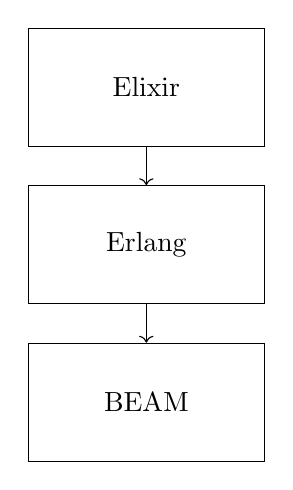
\begin{tikzpicture}[node distance=2cm]
		\node (elixir) [rectangle, draw, text centered, minimum height=1.5cm, minimum width=3cm] {Elixir};
		\node (erlang) [rectangle, draw, below of=elixir, text centered, minimum height=1.5cm, minimum width=3cm] {Erlang};
		\node (beam) [rectangle, draw, below of=erlang, text centered, minimum height=1.5cm, minimum width=3cm] {BEAM};
		
		\draw[->] (elixir) -- (erlang);
		\draw[->] (erlang) -- (beam);
	\end{tikzpicture}
\end{center}

\subsection{Elixir}

Elixir adalah bahasa pemrograman yang modern dan dinamis, dikembangkan untuk memenuhi kebutuhan aplikasi terdistribusi yang skalabel dan fault-tolerant. Meskipun Elixir memiliki sintaks yang berbeda dan modern, ia bergantung sepenuhnya pada ekosistem Erlang untuk menjalankan aplikasinya.

\subsection{Erlang}

Erlang adalah bahasa pemrograman yang mendasari Elixir. Ketika kode Elixir dikompilasi, ia diubah menjadi bytecode Erlang. Ini memungkinkan Elixir untuk memanfaatkan seluruh ekosistem Erlang, termasuk pustaka, alat, dan framework yang sudah ada. Dengan kata lain, Elixir adalah lapisan di atas Erlang yang menyediakan sintaks dan fitur tambahan sambil tetap menggunakan fondasi yang kuat dari Erlang.

\subsection{BEAM}

BEAM (Bogdan/Björn's Erlang Abstract Machine) adalah mesin virtual yang menjalankan bytecode Erlang, termasuk kode yang ditulis dalam Elixir. BEAM dirancang untuk mendukung concurrency, fault-tolerance, dan distribusi yang dibutuhkan oleh aplikasi Elixir dan Erlang. BEAM adalah komponen inti yang membuat Elixir dan Erlang mampu menangani jutaan proses secara efisien.

\subsection{Hubungan dalam Diagram}

Diagram di atas menunjukkan bagaimana Elixir bergantung pada Erlang dan akhirnya dijalankan di atas BEAM. Ketika seorang pengembang menulis kode dalam Elixir, kode tersebut pertama-tama diterjemahkan menjadi bytecode Erlang. Selanjutnya, bytecode tersebut dijalankan oleh BEAM, yang mengelola eksekusi program secara efisien. Ini berarti meskipun Elixir dan Erlang adalah bahasa yang berbeda, mereka berbagi mesin runtime yang sama, yaitu BEAM, yang membuat mereka sangat kompatibel dan interoperabel.

\section{Pattern Matching di Elixir}

Pattern matching adalah salah satu fitur paling kuat dan fundamental dalam bahasa pemrograman Elixir. Fitur ini memungkinkan pengembang untuk mencocokkan struktur data dan mengekstrak nilai-nilai dari struktur tersebut secara deklaratif. Tidak seperti bahasa pemrograman imperatif di mana variabel diinisialisasi dengan nilai, dalam Elixir, pattern matching berfungsi sebagai alat untuk membandingkan dan mengurai data.

\subsection{Dasar-Dasar Pattern Matching}

Pada dasarnya, pattern matching menggunakan operator \texttt{=} untuk mencocokkan sisi kiri dan sisi kanan dari ekspresi. Jika keduanya cocok, maka Elixir akan mengikat nilai dari sisi kanan ke variabel di sisi kiri.

\begin{lstlisting}[language=Elixir]
	iex> x = 1
	1
	
	iex> 1 = x
	1
\end{lstlisting}

Dalam contoh di atas, nilai 1 di sisi kanan diikat ke variabel \texttt{x}. Karena sisi kiri dan kanan dari ekspresi \texttt{1 = x} cocok, Elixir hanya mengembalikan \texttt{1}.

\subsection{Pattern Matching dengan Tuple}

Pattern matching sangat berguna ketika bekerja dengan struktur data yang lebih kompleks seperti tuple.

\begin{lstlisting}[language=Elixir]
	iex> {a, b, c} = {1, 2, 3}
	{1, 2, 3}
	
	iex> a
	1
	
	iex> b
	2
	
	iex> c
	3
\end{lstlisting}

Dalam contoh di atas, tuple \texttt{\{1, 2, 3\}} dicocokkan dengan pola \texttt{\{a, b, c\}}, sehingga nilai-nilai di dalam tuple diikat ke variabel \texttt{a}, \texttt{b}, dan \texttt{c}.

\subsection{Pattern Matching dengan List}

Pattern matching juga dapat digunakan dengan list, termasuk penggunaan \texttt{head} dan \texttt{tail} untuk mencocokkan bagian pertama dari list dan sisa elemennya.

\begin{lstlisting}[language=Elixir]
	iex> [head | tail] = [1, 2, 3]
	[1, 2, 3]
	
	iex> head
	1
	
	iex> tail
	[2, 3]
\end{lstlisting}

Di sini, \texttt{head} mendapatkan nilai pertama dari list, sedangkan \texttt{tail} mendapatkan list yang tersisa.

\subsection{Menggunakan Pattern Matching dalam Fungsi}

Pattern matching dapat digunakan dalam definisi fungsi untuk membuat kode yang lebih bersih dan mudah dibaca.

\begin{lstlisting}[language=Elixir]
	defmodule Example do
	def greet({first_name, last_name}) do
	"Hello, #{first_name} #{last_name}!"
	end
	end
	
	iex> Example.greet({"John", "Doe"})
	"Hello, John Doe!"
\end{lstlisting}

Pada contoh ini, fungsi \texttt{greet/1} menerima tuple yang terdiri dari \texttt{first\_name} dan \texttt{last\_name}. Nilai-nilai ini langsung dicocokkan dengan pola yang didefinisikan dalam parameter fungsi.

Pattern matching di Elixir memungkinkan pemrograman yang lebih deklaratif dan ekspresif. Dengan kemampuan untuk mencocokkan dan mengurai struktur data, pattern matching menjadi salah satu fitur esensial yang mempermudah pengembangan aplikasi dalam Elixir.



\section{Pattern Pipe Operator di Elixir}

\textit{Pipe operator} (\texttt{|>}) adalah salah satu fitur yang sangat berguna di Elixir, yang memungkinkan chaining atau penggabungan dari beberapa operasi menjadi satu alur yang mudah dibaca. Pipe operator mengambil output dari ekspresi sebelumnya dan meneruskannya sebagai argumen pertama ke fungsi berikutnya.

\subsection{Dasar-Dasar Pipe Operator}

Pada dasarnya, pipe operator memungkinkan kita untuk menulis kode yang lebih rapi dan berurutan daripada harus menyusun fungsi secara bersarang (nested).

\begin{lstlisting}[language=Elixir]
	iex> "hello"
	...> |> String.upcase()
	...> |> String.reverse()
	"OLLEH"
\end{lstlisting}

Dalam contoh di atas, string \texttt{"hello"} pertama-tama diubah menjadi huruf kapital dengan \texttt{String.upcase/1}, kemudian hasilnya diteruskan ke \texttt{String.reverse/1} yang membalikkan urutan karakter. Tanpa pipe operator, kode ini akan terlihat seperti berikut:

\begin{lstlisting}[language=Elixir]
	iex> String.reverse(String.upcase("hello"))
	"OLLEH"
\end{lstlisting}

\subsection{Pipe Operator dengan List}

Pipe operator juga sering digunakan dengan fungsi-fungsi yang memanipulasi list, seperti pada contoh berikut:

\begin{lstlisting}[language=Elixir]
	iex> [1, 2, 3, 4, 5]
	...> |> Enum.map(&(&1 * 2))
	...> |> Enum.filter(&(&1 > 5))
	[6, 8, 10]
\end{lstlisting}

Pada contoh ini, list \texttt{[1, 2, 3, 4, 5]} pertama-tama dikalikan dengan 2 menggunakan \texttt{Enum.map/2}, kemudian hasilnya disaring dengan \texttt{Enum.filter/2} untuk hanya menyertakan angka yang lebih besar dari 5.

\subsection{Penjelasan `\&1`, `\&2`, dan Seterusnya}

Dalam Elixir, `\&` digunakan untuk membuat anonymous functions atau fungsi tanpa nama. Dalam anonymous function, `\&1`, `\&2`, dan seterusnya adalah placeholder untuk argumen yang diterima oleh fungsi tersebut.

\begin{lstlisting}[language=Elixir]
	iex> add = &(&1 + &2)
	#Function<6.86581258/2 in :erl_eval.expr/5>
	iex> add.(2, 3)
	5
\end{lstlisting}

Pada contoh ini, `\&1` dan `\&2` mewakili argumen pertama dan kedua dari anonymous function yang dibuat. Fungsi ini menambahkan kedua argumen dan mengembalikan hasilnya.

Pipe operator di Elixir mempermudah penulisan kode yang jelas dan mudah dibaca, terutama ketika menggabungkan serangkaian operasi. Selain itu, kemampuan untuk menggunakan pipe operator dengan fungsi yang menerima banyak parameter serta penggunaan `\&1`, `\&2`, dan seterusnya memungkinkan penulisan kode yang lebih fleksibel dan ekspresif.

\subsection{Pipe Operator dengan Fungsi yang Memiliki Banyak Parameter}

Pipe operator juga dapat digunakan dengan fungsi yang memerlukan lebih dari satu parameter. Berikut adalah contohnya:

\begin{lstlisting}[language=Elixir]
	defmodule Example do
	def multiply_and_add(x, y, z) do
	x * y + z
	end
	end
	
	iex> 5
	...> |> Example.multiply_and_add(2, 3)
	13
\end{lstlisting}

Dalam contoh di atas, angka \texttt{5} diteruskan sebagai parameter pertama ke fungsi \texttt{multiply\_and\_add/3}, dan parameter kedua dan ketiga adalah \texttt{2} dan \texttt{3}. Fungsi ini mengalikan \texttt{5} dengan \texttt{2} dan menambahkan \texttt{3}, menghasilkan \texttt{13}.



\subsection{Contoh dengan Konversi Tipe Data}

Dalam Elixir, ketika kita menggunakan pipe operator dengan fungsi yang memerlukan parameter dengan tipe yang berbeda dari output fungsi sebelumnya, kita harus memastikan bahwa data yang diteruskan sesuai dengan tipe yang diharapkan oleh fungsi tersebut. Ini mungkin memerlukan konversi atau pemrosesan data sebelum menggunakan pipe operator.

Misalkan kita memiliki fungsi yang mengharapkan parameter bertipe integer dan fungsi lain yang menghasilkan string. Kita perlu mengkonversi string menjadi integer sebelum meneruskan ke fungsi berikutnya.

Berikut adalah contoh sederhana:

\begin{lstlisting}[language=Elixir]
	defmodule Converter do
	def string_to_integer(str) do
	String.to_integer(str)
	end
	
	def add_five(num) do
	num + 5
	end
	end
	
	iex> "42"
	...> |> Converter.string_to_integer()
	...> |> Converter.add_five()
	47
\end{lstlisting}

Pada contoh ini, string \texttt{"42"} pertama-tama dikonversi menjadi integer dengan \texttt{Converter.string\_to\_integer/1}, kemudian hasil integer tersebut diteruskan ke \texttt{Converter.add\_five/1} untuk ditambahkan dengan 5.

\subsection{Menggunakan Nilai Pipe sebagai Parameter Kedua}

Di Elixir, kita dapat menggunakan pipe operator untuk meneruskan nilai dari fungsi pertama sebagai parameter kedua dalam sebuah fungsi dengan memanfaatkan fungsi anonim. Contoh berikut menunjukkan cara melakukannya:

\begin{lstlisting}[language=Elixir]
	defmodule Example do
	def hello(greet, name) do
	greet <> name
	end
	end
	
	iex> "world"
	...> |> (&Example.hello("Hello, ", &1 )).()
	"Hello, world"
\end{lstlisting}

Pada kode di atas, modul \texttt{Example} mendefinisikan fungsi \texttt{hello/2} yang menggabungkan dua string: \texttt{greet} dan \texttt{name}. Nilai \texttt{"world"} diteruskan melalui pipe operator ke fungsi anonim. Fungsi anonim tersebut menggunakan \texttt{"Hello, "} sebagai parameter pertama dan nilai dari pipe (\texttt{"world"}) sebagai parameter kedua. 

Fungsi \texttt{hello/2} kemudian menggabungkan \texttt{"Hello, "} dengan \texttt{"world"}, menghasilkan string \texttt{"Hello, world"}. Dengan pendekatan ini, pipe operator dan fungsi anonim memungkinkan kita untuk dengan mudah mengatur parameter fungsi, termasuk menggunakan nilai dari pipe sebagai parameter kedua. Pendekatan ini meningkatkan fleksibilitas dan keterbacaan kode dalam Elixir.

\section{Menyimpan dan Memuat Ulang Nilai ke dan dari File}

Elixir menyediakan berbagai metode untuk menyimpan dan memuat ulang data dari file. Ini berguna untuk menyimpan konfigurasi, hasil pemrosesan, atau data lainnya secara persisten. Berikut adalah cara melakukannya dengan menggunakan Elixir.

\subsection{Menyimpan Data ke File}

Untuk menyimpan data ke file, Anda dapat menggunakan fungsi `File.write/2`. Fungsi ini menerima nama file dan data yang akan ditulis. Berikut adalah contoh cara menyimpan string ke file:

\begin{lstlisting}[language=Elixir]
	filename = "data.txt"
	data = "Hello, Elixir!"
	
	File.write(filename, data)
\end{lstlisting}

Pada contoh di atas, string \texttt{"Hello, Elixir!"} disimpan ke dalam file \texttt{"data.txt"}.

\subsection{Memuat Data dari File}

Untuk memuat data dari file, Anda dapat menggunakan fungsi `File.read/1`. Fungsi ini membaca isi file dan mengembalikan hasilnya sebagai string. Berikut adalah contoh cara memuat data dari file:

\begin{lstlisting}[language=Elixir]
# File: lib/file_reader.ex

defmodule FileReader do
def read_file(filename) do
case File.read(filename) do
{:ok, content} ->
IO.puts("File content: #{content}")
{:error, reason} ->
IO.puts("Failed to read file: #{reason}")
end
end
end
\end{lstlisting}

Perintah pada \texttt{iex} command prompt: 

\begin{lstlisting}[language=bash]
	FileReader.read_file("data.txt")
\end{lstlisting}

Pada contoh di atas, fungsi `File.read/1` membaca isi file \texttt{"data.txt"}. Jika berhasil, isi file ditampilkan ke konsol; jika terjadi kesalahan, pesan kesalahan akan ditampilkan.

\subsection{Menyimpan dan Memuat Data dengan Format Lain}

Jika Anda bekerja dengan data yang lebih kompleks, seperti objek atau struktur data, Anda mungkin ingin menggunakan format lain, seperti JSON atau Erlang Term Storage (ETS). Berikut adalah contoh cara menggunakan format JSON untuk menyimpan dan memuat data:

\begin{lstlisting}[language=Elixir]
	# File: lib/json_file_handler.ex
	
	defmodule JsonFileHandler do
	# Save data to a JSON file
	def save_json(filename, data) do
	File.write(filename, Jason.encode!(data))
	end
	
	# Load data from a JSON file
	def load_json(filename) do
	case File.read(filename) do
	{:ok, content} ->
	case Jason.decode(content) do
	{:ok, decoded_data} ->
	IO.inspect(decoded_data)
	{:error, reason} ->
	IO.puts("Failed to decode JSON: #{reason}")
	end
	{:error, reason} ->
	IO.puts("Failed to read file: #{reason}")
	end
	end
	end

\end{lstlisting}

Perintah pada \texttt{iex} command prompt: 

\begin{lstlisting}[language=bash]
	filename="data.json"
	data='{"greeting": "Hello, Elixir!", "count": 42}'
	JsonFileHandler.save_json(filename, data)
	JsonFileHandler.load_json(filename)
\end{lstlisting}

Pada contoh di atas, kita menggunakan pustaka `Jason` untuk mengkodekan dan mendekode data JSON. Fungsi `Jason.encode!/1` mengubah data menjadi format JSON, dan `Jason.decode/1` mengembalikannya ke bentuk asli.

Dengan menggunakan fungsi-fungsi dari modul `File` dan pustaka tambahan seperti `Jason`, Anda dapat dengan mudah menyimpan dan memuat data dari file di Elixir. Ini memungkinkan pengelolaan data yang persisten dan interoperabilitas dengan berbagai format data.


\section{Latihan}

Pada bagian ini, terdapat beberapa latihan yang bertujuan untuk menguji pemahaman mengenai kode-kode yang telah dipelajari. Setiap latihan berisi kode yang harus dijalankan dan dipahami hasilnya.

\subsection{Latihan 1: Pattern Matching di Elixir}

Latihan pertama ini akan mengeksplorasi bagaimana pattern matching bekerja di Elixir. Anda akan diminta untuk memahami dan menjalankan contoh kode di bawah ini.

\begin{lstlisting}[language=Elixir]
	# Contoh Pattern Matching Sederhana
	{x, y, z} = {1, 2, 3}
	IO.puts("x = #{x}, y = #{y}, z = #{z}")
	
	# Pattern Matching dengan List
	[head | tail] = [1, 2, 3, 4, 5]
	IO.puts("Head: #{head}")
	IO.inspect(tail)
	
	# Pattern Matching dengan Map
	%{name: name, age: age} = %{name: "John", age: 30}
	IO.puts("Name: #{name}, Age: #{age}")
\end{lstlisting}

\subsection{Latihan 2: Pipe Operator di Elixir}

Latihan kedua ini akan berfokus pada penggunaan pipe operator (\texttt{|>}) di Elixir. Jalankan dan pahami bagaimana nilai dapat diteruskan dari satu fungsi ke fungsi lainnya.

\begin{lstlisting}[language=Elixir]
	# Contoh Penggunaan Pipe Operator
	defmodule PipeExample do
	def greet(name), do: "Hello, " <> name
	def exclaim(statement), do: statement <> "!"
	def emphasize(statement), do: String.upcase(statement)
	end
	
	"world"
	|> PipeExample.greet()
	|> PipeExample.exclaim()
	|> PipeExample.emphasize()
	|> IO.puts()
\end{lstlisting}

Selain itu, berikut contoh pipe operator yang memindahkan nilai ke parameter kedua:

\begin{lstlisting}[language=Elixir]
	defmodule Example do
	def wrap_in_brackets(prefix, content), do: prefix <> "[" <> content <> "]"
	end
	
	"world"
	|> (&Example.wrap_in_brackets(&1, "Hello")).()
	|> IO.puts()
\end{lstlisting}

\texttt{\&1} merujuk pada nilai yang diteruskan melalui pipe operator. Variasi lainnya seperti \texttt{\&2} merujuk pada parameter kedua, dan seterusnya.

\subsection{Latihan 3: Membaca File Teks}

Latihan ini melibatkan penggunaan modul \texttt{FileReader} untuk membaca konten dari sebuah file teks. Pastikan file \texttt{data.txt} tersedia dengan beberapa konten di dalamnya.

\begin{lstlisting}[language=Elixir]
	# File: lib/file_reader.ex
	
	defmodule FileReader do
	def read_file(filename) do
	case File.read(filename) do
	{:ok, content} ->
	IO.puts("File content: #{content}")
	{:error, reason} ->
	IO.puts("Failed to read file: #{reason}")
	end
	end
	end
\end{lstlisting}

\begin{lstlisting}[language=bash]
	iex> 	FileReader.read_file("data.txt")\part{title}
\end{lstlisting}

\subsection{Latihan 4: Menyimpan dan Membaca Data JSON}

Latihan ini menggunakan modul \texttt{JsonFileHandler} untuk menyimpan dan membaca data dalam format JSON. Anda akan melihat bagaimana data JSON dapat disimpan ke file dan kemudian dimuat kembali.

\begin{lstlisting}[language=Elixir]
	# File: lib/json_file_handler.ex
	
	defmodule JsonFileHandler do
	# Save data to a JSON file
	def save_json(filename, data) do
	File.write(filename, Jason.encode!(data))
	end
	
	# Load data from a JSON file
	def load_json(filename) do
	case File.read(filename) do
	{:ok, content} ->
	case Jason.decode(content) do
	{:ok, decoded_data} ->
	IO.inspect(decoded_data)
	{:error, reason} ->
	IO.puts("Failed to decode JSON: #{reason}")
	end
	{:error, reason} ->
	IO.puts("Failed to read file: #{reason}")
	end
	end
	end
	
\end{lstlisting}

\begin{lstlisting}[language=bash]
iex> filename="data.json"
iex> data='{"greeting": "Hello, Elixir!", "count": 42}'
iex> JsonFileHandler.save_json(filename, data)
iex> JsonFileHandler.load_json(filename)
\end{lstlisting}


\subsection{Latihan 5: Menggabungkan Semua Konsep}

Dalam latihan ini, buatlah sebuah modul yang memanfaatkan pattern matching, pipe operator, serta pembacaan dan penulisan file JSON. Fungsi dalam modul ini:
\begin{itemize}
	\item Membaca data dari sebuah file JSON.
	\item Menggunakan pattern matching untuk mengekstrak nilai tertentu dari data JSON yang diambil.
	\item Memanipulasi data tersebut menggunakan pipe operator.
	\item Menyimpan hasilnya kembali ke file JSON yang sama.
\end{itemize}

Berikut adalah struktur dasar untuk memulai:

\begin{lstlisting}[language=Elixir]
	defmodule IntegratedExercise do
	def process_file(filename) do
	# Membaca file JSON
	filename
	|> File.read()               # Baca file
	|> case do                   # Gunakan pattern matching untuk memproses konten
	{:ok, content} ->
	# Decode JSON dan ekstrak nilai menggunakan pattern matching
	case Jason.decode(content) do
	{:ok, %{"greeting" => greeting, "count" => count}} ->
	# Manipulasi data menggunakan pipe operator
	new_count = count + 1
	new_data = %{"greeting" => greeting, "count" => new_count}
	
	# Simpan data baru ke file JSON
	File.write(filename, Jason.encode!(new_data))
	{:error, reason} ->
	IO.puts("Failed to decode JSON: #{reason}")
	end
	{:error, reason} ->
	IO.puts("Failed to read file: #{reason}")
	end
	end
	end
	
	# Memanggil fungsi
	filename = "data.json"
	IntegratedExercise.process_file(filename)
\end{lstlisting}

\textbf{Instruksi:}
\begin{enumerate}
	\item Buat file \texttt{data.json} dengan struktur: \texttt{\{"greeting": "Hello, Elixir!", "count": 42\}}.
	\item Modifikasi fungsi \texttt{process\_file} untuk melakukan operasi tambahan, seperti menambahkan data baru atau mengubah nilai tertentu.
	\item Pastikan hasil akhirnya disimpan kembali ke dalam file JSON yang sama.
\end{enumerate}

\section{Memperluas Modul Lottery}

Dalam bagian ini, kami memperluas fungsionalitas modul \texttt{Lottery} dengan menambahkan beberapa fitur baru. Fitur-fitur ini mencakup menyimpan dan memuat pool lotere ke dan dari file, serta membuat tangan lotere yang acak. Kode berikut menunjukkan peningkatan-peningkatan ini:

\begin{lstlisting}[language=Elixir]
	defmodule Lottery do
	def generate_pool do
	numbers = ["Number 1", "Number 2", "Number 3", "Number 4", "Number 5"]
	pots = ["Pot 1", "Pot 2", "Pot 3", "Pot 4"]
	
	# Membuat pool dengan menggabungkan angka dan pot.
	for pot <- pots, number <- numbers do
	"#{number} in #{pot}"
	end
	end
	
	def randomize(pool) do
	Enum.shuffle(pool)
	end
	
	def contains?(pool, number) do
	Enum.member?(pool, number)
	end
	
	def distribute(pool, draw_size) do
	Enum.split(pool, draw_size)
	end
	
	def save_pool(pool, filename) do
	binary = :erlang.term_to_binary(pool)
	File.write(filename, binary)
	end
	
	def load_pool(filename) do
	case File.read(filename) do
	{:ok, binary} -> :erlang.binary_to_term(binary)
	{:error, _reason} -> "File tersebut tidak ada"
	end
	end
	
	def create_hand(draw_size) do
	Lottery.generate_pool()
	|> Lottery.randomize()
	|> Lottery.distribute(draw_size)
	end
	end
\end{lstlisting}

\subsection{Deskripsi Fungsi}

\begin{itemize}
	\item \texttt{save\_pool/2}: Fungsi ini mengkonversi pool lotere menjadi format biner dan menyimpannya ke dalam file. File ini kemudian dapat digunakan untuk mempertahankan status pool.
	\item \texttt{load\_pool/1}: Fungsi ini membaca file biner dan mengkonversinya kembali ke dalam format pool lotere. Jika file tidak ditemukan, fungsi ini akan mengembalikan pesan kesalahan.
	\item \texttt{create\_hand/1}: Fungsi ini membuat tangan lotere yang acak dengan menggabungkan fungsi-fungsi yang telah didefinisikan sebelumnya. Fungsi ini membuat pool, merandomnya, dan kemudian membaginya sesuai dengan ukuran undian yang ditentukan.
\end{itemize}


	\chapter{Dokumentasi dan Unit Test pada Elixir}


\section{Dokumentasi di Elixir}

Elixir mendukung dokumentasi yang mudah untuk modul dan fungsi. Dokumentasi ini dapat ditambahkan langsung dalam kode menggunakan komentar khusus yang disebut dengan \texttt{@moduledoc} untuk modul dan \texttt{@doc} untuk fungsi. Selain itu, Elixir juga menyediakan cara mudah untuk menggenerate dokumentasi dalam bentuk HTML menggunakan perintah \texttt{mix docs}.


\subsection{Dokumentasi pada Level Modul}

Untuk mendokumentasikan sebuah modul, digunakan anotasi \texttt{@moduledoc}. Ini adalah tempat yang tepat untuk memberikan deskripsi tentang tujuan modul, bagaimana modul tersebut digunakan, serta contoh-contoh jika diperlukan.

\begin{lstlisting}[language=Elixir]
	defmodule ExampleModule do
	@moduledoc """
	This module is an example of how to document a module in Elixir.
	
	It serves to demonstrate how module documentation can be written
	and used as a reference when generating HTML documentation.
	"""
	
	# Other functions and logic can be written here
	end
\end{lstlisting}

\subsection{Dokumentasi pada Level Fungsi}

Selain mendokumentasikan modul, Anda juga bisa mendokumentasikan setiap fungsi dengan menggunakan anotasi \texttt{@doc}. Dokumentasi fungsi biasanya memberikan penjelasan tentang apa yang dilakukan fungsi tersebut, parameter yang dibutuhkan, dan hasil yang dikembalikan.

\begin{lstlisting}[language=Elixir]
	defmodule ExampleModule do
	@moduledoc """
	This module is an example of how to document a module in Elixir.
	"""
	
	@doc """
	This function adds two numbers.
	
	## Parameters
	- a: the first number.
	- b: the second number.
	
	## Example
	
	iex> ExampleModule.add(2, 3)
	5
	"""
	def add(a, b) do
	a + b
	end
	end
\end{lstlisting}

\section{Menambahkan \texttt{ex\_doc} untuk Dokumentasi}

Untuk menghasilkan dokumentasi dalam proyek Elixir, Anda perlu menambahkan library \texttt{ex\_doc}. Library ini memungkinkan Anda untuk menghasilkan dokumentasi dalam berbagai format, termasuk HTML. Berikut adalah langkah-langkah untuk menambahkan \texttt{ex\_doc} ke dalam proyek Elixir Anda.

\subsection{Langkah-langkah Menambahkan \texttt{ex\_doc}}

\begin{enumerate}
	\item Buka file \texttt{mix.exs} di proyek Anda, dan tambahkan \texttt{ex\_doc} ke dalam daftar dependensi di fungsi \texttt{deps}. Pastikan Anda menambahkan dependensi ini hanya untuk lingkungan pengembangan (\texttt{dev}) dan tidak di runtime.
	
	\begin{lstlisting}[language=Elixir]
		defp deps do
		[
			{:ex_doc, "~> 0.34"}
		]
		end
	\end{lstlisting}
	
	\item Setelah menambahkan \texttt{ex\_doc}, jalankan perintah berikut di terminal untuk mengunduh dan menginstal dependensi:
	
	\begin{lstlisting}[language=Bash]
		mix deps.get
	\end{lstlisting}
	
	\item Setelah dependensi berhasil diinstal, Anda dapat menghasilkan dokumentasi untuk proyek Anda dengan perintah berikut:
	
	\begin{lstlisting}[language=Bash]
		mix docs
	\end{lstlisting}
	
	\item Dokumentasi yang dihasilkan akan disimpan dalam folder \texttt{doc/} di dalam direktori proyek Anda. Anda dapat membuka file \texttt{index.html} di browser untuk melihat dokumentasi dalam format HTML.
\end{enumerate}

\section{Mengenerate Dokumentasi HTML}

Untuk menggenerate dokumentasi dalam format HTML, Elixir menyediakan perintah sederhana, yaitu \texttt{mix docs}. Perintah ini akan mencari dokumentasi di dalam modul dan fungsi yang ada, lalu mengubahnya menjadi halaman HTML yang mudah dibaca. Langkah-langkahnya adalah sebagai berikut:

\begin{enumerate}
	\item Pastikan Anda berada di dalam direktori proyek Elixir.
	\item Jalankan perintah berikut pada \textit{command prompt}:
	\begin{lstlisting}[language=Bash]
mix docs
	\end{lstlisting}
	
	\item Dokumentasi HTML akan dihasilkan di dalam folder \texttt{doc}.
\end{enumerate}

Dengan mendokumentasikan kode dengan baik dan mengenerate dokumentasi HTML, Anda dapat mempermudah orang lain (atau diri sendiri di masa depan) untuk memahami kode yang Anda tulis.



\section{Unit Test di Elixir}

Unit testing di Elixir dapat dilakukan menggunakan modul bawaan bernama \texttt{ExUnit}. Elixir menyediakan fitur untuk membuat test dalam file khusus serta memungkinkan test ditulis dalam dokumentasi fungsi menggunakan anotasi \texttt{doctest}. Unit test sangat penting untuk memastikan bahwa fungsi-fungsi dalam kode bekerja sesuai harapan.



\subsection{Kesimpulan}

Dengan menambahkan \texttt{ex\_doc}, Anda dapat dengan mudah menghasilkan dokumentasi untuk proyek Elixir Anda. Dokumentasi ini membantu memudahkan pemahaman tentang kode yang ditulis dan berfungsi sebagai panduan bagi pengguna lain yang ingin menggunakan atau mengembangkan proyek tersebut.


\subsection{Unit Test dalam File Khusus}

Untuk membuat unit test di Elixir, biasanya digunakan file khusus yang ditempatkan dalam folder \texttt{test}. File test ini harus memiliki akhiran \texttt{\_test.exs}. Di dalam file tersebut, Anda mendefinisikan modul yang menggunakan \texttt{ExUnit.Case} sebagai template.

\begin{lstlisting}[language=Elixir]
	defmodule ExampleModuleTest do
	use ExUnit.Case
	
	test "adds two numbers" do
	assert ExampleModule.add(2, 3) == 5
	end
	
	test "subtracts two numbers" do
	assert ExampleModule.subtract(5, 2) == 3
	end
	end
\end{lstlisting}

\subsection{Unit Test dalam Dokumentasi Fungsi (Doctest)}

Selain menulis test di file khusus, Elixir juga memungkinkan Anda untuk menulis unit test langsung dalam dokumentasi fungsi menggunakan anotasi \texttt{doctest}. Test ini secara otomatis dijalankan ketika Anda menjalankan \texttt{ExUnit}. Contoh doctest dapat ditulis dalam bagian \texttt{@doc} dari suatu fungsi.

\begin{lstlisting}[language=Elixir]
	defmodule ExampleModule do
	@moduledoc """
	This module demonstrates how to document and test functions.
	"""
	
	@doc """
	This function adds two numbers.
	
	## Parameters
	- a: the first number.
	- b: the second number.
	
	## Example
	
	iex> ExampleModule.add(2, 3)
	5
	"""
	def add(a, b) do
	a + b
	end
	
	@doc """
	This function subtracts two numbers.
	
	## Parameters
	- a: the first number.
	- b: the second number.
	
	## Example
	
	iex> ExampleModule.subtract(5, 2)
	3
	"""
	def subtract(a, b) do
	a - b
	end
	end
\end{lstlisting}

Untuk mengaktifkan \texttt{doctest}, Anda perlu menambahkannya dalam modul test:

\begin{lstlisting}[language=Elixir]
	defmodule ExampleModuleTest do
	use ExUnit.Case
	doctest ExampleModule
	end
\end{lstlisting}

\subsection{Menjalankan Test dari Command Prompt}

Elixir memudahkan Anda untuk menjalankan test langsung dari command prompt. Ada beberapa opsi untuk menjalankan test tergantung kebutuhan Anda.

\subsubsection{Menjalankan Semua Test}

Untuk menjalankan semua test yang ada di proyek, cukup gunakan perintah berikut:

\begin{lstlisting}[language=Bash]
	mix test
\end{lstlisting}

Perintah ini akan mengeksekusi semua test yang ada di folder \texttt{test} dan menampilkan hasilnya di terminal.

\subsubsection{Menjalankan Test Spesifik untuk Modul Tertentu}

Jika Anda hanya ingin menjalankan test untuk modul tertentu, Anda dapat menyebutkan nama file test yang bersangkutan. Misalnya, untuk menjalankan test pada \texttt{ExampleModuleTest}, jalankan perintah berikut:

\begin{lstlisting}[language=Bash]
	mix test test/example_module_test.exs
\end{lstlisting}

\subsubsection{Menjalankan Test Spesifik untuk Fungsi Tertentu}

Untuk menjalankan test yang spesifik untuk suatu fungsi dalam modul, Anda dapat menggunakan tag line number. Misalnya, jika test untuk fungsi \texttt{add} ada pada baris 4 dalam file test, Anda bisa menjalankan perintah berikut:

\begin{lstlisting}[language=Bash]
	mix test test/example_module_test.exs:4
\end{lstlisting}

Jika Anda ingin menjalankan test untuk fungsi lain seperti \texttt{subtract} yang ada di baris 8, Anda cukup menjalankan:

\begin{lstlisting}[language=Bash]
	mix test test/example_module_test.exs:8
\end{lstlisting}

Dengan cara ini, hanya test yang ada pada baris tersebut yang akan dijalankan, sehingga memudahkan dalam proses debugging dan pengujian parsial.

Dengan menggunakan \texttt{ExUnit}, Elixir memberikan cara yang mudah dan efisien untuk melakukan unit testing. Anda bisa menulis test baik dalam file khusus maupun langsung dalam dokumentasi fungsi menggunakan \texttt{doctest}. Menjalankan test dari command prompt juga fleksibel, memungkinkan Anda untuk menjalankan seluruh test, test untuk modul tertentu, atau test untuk fungsi spesifik.

\section{Latihan}

Bagian ini berisi beberapa latihan yang dirancang untuk membantu Anda mempraktikkan dokumentasi dan unit testing di Elixir. Setiap latihan akan mencakup pembuatan modul, menulis dokumentasi, dan membuat unit test. 

\subsection{Latihan 1: Menulis Dokumentasi Modul}

Buatlah sebuah modul Elixir bernama \texttt{Calculator} yang memiliki dua fungsi: \texttt{multiply/2} dan \texttt{divide/2}. Tulislah dokumentasi untuk setiap fungsi menggunakan anotasi \texttt{@doc}.

\begin{lstlisting}[language=Elixir]
	defmodule Calculator do
	@moduledoc """
	A module for basic arithmetic operations.
	"""
	
	@doc """
	Multiplies two numbers.
	
	## Parameters
	- x: the first number.
	- y: the second number.
	
	## Example
	
	iex> Calculator.multiply(4, 5)
	20
	"""
	def multiply(x, y) do
	x * y
	end
	
	@doc """
	Divides two numbers.
	
	## Parameters
	- x: the numerator.
	- y: the denominator.
	
	## Example
	
	iex> Calculator.divide(10, 2)
	5
	"""
	def divide(x, y) do
	x / y
	end
	end
\end{lstlisting}

\subsection{Latihan 2: Menulis Unit Test untuk Modul}

Buatlah file test bernama \texttt{calculator\_test.exs} di dalam folder \texttt{test} untuk mengetes fungsi \texttt{multiply/2} dan \texttt{divide/2} dari modul \texttt{Calculator}. Sertakan beberapa skenario pengujian.

\begin{lstlisting}[language=Elixir]
	defmodule CalculatorTest do
	use ExUnit.Case
	doctest Calculator
	
	test "multiplies two numbers" do
	assert Calculator.multiply(4, 5) == 20
	end
	
	test "divides two numbers" do
	assert Calculator.divide(10, 2) == 5
	end
	
	test "divides by zero raises an error" do
	assert_raise ArithmeticError, fn -> Calculator.divide(10, 0) end
	end
	end
\end{lstlisting}

\subsection{Latihan 3: Menjalankan Test untuk Modul}

Jalankan unit test yang telah Anda tulis untuk modul \texttt{Calculator} menggunakan perintah berikut:

\begin{lstlisting}[language=Bash]
	mix test test/calculator_test.exs
\end{lstlisting}

\subsection{Latihan 4: Menjalankan Test untuk Fungsi Tertentu}

Tambahkan sebuah test baru dalam \texttt{calculator\_test.exs} untuk fungsi \texttt{multiply/2} dan jalankan test tersebut menggunakan nomor baris.

\begin{lstlisting}[language=Elixir]
	defmodule CalculatorTest do
	use ExUnit.Case
	doctest Calculator
	
	test "multiplies two numbers" do
	assert Calculator.multiply(4, 5) == 20
	end
	
	# New test added for specific function
	test "checks multiply with negative numbers" do
	assert Calculator.multiply(-4, 5) == -20
	end
	end
\end{lstlisting}

Jika test baru ditambahkan pada baris 6, jalankan perintah berikut:

\begin{lstlisting}[language=Bash]
	mix test test/calculator_test.exs:6
\end{lstlisting}


\section{Soal}

Bagian ini berisi beberapa soal latihan tambahan yang dirancang untuk mempraktikkan dokumentasi dan unit testing di Elixir. Setiap soal merupakan varian dari contoh-contoh latihan sebelumnya.

\subsection{Soal 1: Dokumentasi dan Unit Test untuk Modul \texttt{Statistics}}

Buatlah modul Elixir bernama \texttt{Statistics} yang memiliki dua fungsi: \texttt{mean/1} dan \texttt{median/1}. 

\begin{enumerate}
	\item Dokumentasikan setiap fungsi dengan anotasi \texttt{@doc}. Fungsi \texttt{mean/1} harus menghitung rata-rata dari sebuah list angka, sementara \texttt{median/1} harus menghitung median dari list angka yang sudah diurutkan.
	\item Buatlah file test bernama \texttt{statistics\_test.exs} di dalam folder \texttt{test} untuk mengetes fungsi \texttt{mean/1} dan \texttt{median/1}. Sertakan beberapa skenario pengujian, seperti menghitung rata-rata dan median untuk list dengan berbagai panjang dan nilai.
\end{enumerate}

\subsection{Soal 2: Dokumentasi dan Unit Test untuk Modul \texttt{StringUtils}}

Buatlah modul Elixir bernama \texttt{StringUtils} yang memiliki dua fungsi: \texttt{reverse/1} dan \texttt{capitalize/1}. 

\begin{enumerate}
	\item Dokumentasikan setiap fungsi dengan anotasi \texttt{@doc}. Fungsi \texttt{reverse/1} harus membalikkan string, sementara \texttt{capitalize/1} harus mengubah huruf pertama dari string menjadi huruf kapital.
	\item Buatlah file test bernama \texttt{string\_utils\_test.exs} di dalam folder \texttt{test} untuk mengetes fungsi \texttt{reverse/1} dan \texttt{capitalize/1}. Sertakan beberapa skenario pengujian, seperti membalikkan string dengan berbagai karakter dan mengubah kapitalisasi string dengan berbagai kasus huruf.
\end{enumerate}



	\chapter{Struktur Data di Elixir: Atom, Map, Tuple, List, dan Keyword List}

\section{Atom}
Atom dalam Elixir adalah konstanta yang nilainya adalah nama itu sendiri. Atom sering digunakan untuk memberi label nilai atau mewakili konsep-konsep tertentu dalam program. Atom diawali dengan titik dua (\texttt{:}), diikuti oleh namanya.

\subsection{Membuat Atom}
Atom dibuat dengan menambahkan nama diawali dengan titik dua.
\begin{lstlisting}[language=Elixir]
	:name  # Sebuah atom dengan nilai :name
\end{lstlisting}

\subsection{Menggunakan Atom dalam Pattern Matching}
Atom umumnya digunakan dalam pattern matching untuk alur kontrol.
\begin{lstlisting}[language=Elixir]
	status = :ok
	
	case status do
	:ok -> "Berhasil"
	:error -> "Gagal"
	end
\end{lstlisting}

\subsection{Atom dalam Keyword Lists}
Atom biasanya digunakan sebagai kunci dalam keyword lists, yaitu daftar pasangan kunci-nilai.
\begin{lstlisting}[language=Elixir]
	keyword_list = [name: "Alice", age: 30]
	
	IO.puts(keyword_list[:name])  # Output: Alice
\end{lstlisting}

\subsection{Atom yang Mewakili Modul dan Fungsi}
Dalam Elixir, atom digunakan untuk mewakili nama modul dan referensi fungsi.
\begin{lstlisting}[language=Elixir]
	String.length("hello")  # Di sini, modul String adalah atom
	
	fun = &String.length/1
	IO.puts(fun.("world"))  # Output: 5
\end{lstlisting}

Atom efisien dan ringan, menjadikannya ideal untuk digunakan dalam pattern matching, sebagai label, dan dalam berbagai struktur data seperti keyword lists dan maps. Karena atom bersifat immutable, atom menyediakan cara yang dapat diandalkan untuk merujuk nilai dengan nama di seluruh program.

\section{Map}
Map dalam Elixir adalah struktur data kunci-nilai di mana kunci dapat berupa tipe apa saja. Map tidak terurut, yang berarti pasangan kunci-nilai tidak disimpan dalam urutan tertentu.

\subsection{Membuat Map}
Map dibuat menggunakan sintaks \texttt{\%{}}.
\begin{lstlisting}[language=Elixir]
	map = %{"name" => "Alice", "age" => 30}
\end{lstlisting}

\subsection{Menambah/Memperbarui Entitas dalam Map}
Untuk menambah atau memperbarui entitas dalam map, gunakan fungsi \texttt{Map.put/3}.
\begin{lstlisting}[language=Elixir]
	map = %{"name" => "Alice", "age" => 30}
	updated_map = Map.put(map, "city", "New York")
\end{lstlisting}

\subsection{Menghapus Entitas dari Map}
Untuk menghapus entitas dari map, gunakan fungsi \texttt{Map.delete/2}.
\begin{lstlisting}[language=Elixir]
	map = %{"name" => "Alice", "age" => 30}
	updated_map = Map.delete(map, "age")
\end{lstlisting}

\subsection{Mengakses Nilai dalam Map}
Nilai dapat diakses menggunakan kuncinya.
\begin{lstlisting}[language=Elixir]
	map = %{"name" => "Alice", "age" => 30}
	IO.puts(map["name"])  # Output: Alice
\end{lstlisting}

\section{Tuple}
Tuple adalah koleksi elemen yang terurut. Tuple bersifat immutable, yang berarti tidak dapat diubah setelah dibuat.

\subsection{Membuat Tuple}
Tuple dibuat menggunakan sintaks \texttt{\{\}}.
\begin{lstlisting}[language=Elixir]
	tuple = {"Alice", 30, "New York"}
\end{lstlisting}

\subsection{Mengakses Elemen dalam Tuple}
Elemen dalam tuple dapat diakses berdasarkan indeksnya menggunakan pattern matching atau fungsi \texttt{elem/2}.
\begin{lstlisting}[language=Elixir]
	tuple = {"Alice", 30, "New York"}
	IO.puts(elem(tuple, 0))  # Output: Alice
\end{lstlisting}

\subsection{Memperbarui Tuple}
Berikut adalah perintah untuk menambahkan elemen baru ke suatu tuple. Akan tetapi, karena tuple bersifat immutable, untuk memperbarui tuple, harus dibuat tuple baru dengan nilai yang diperbarui, seolah-olah elemen baru ditambahkan ke tuple.
\begin{lstlisting}[language=Elixir]
	tuple = {"Alice", 30, "New York"}
	updated_tuple = Tuple.append(tuple, "Engineer")
\end{lstlisting}

\subsection{Menghapus Elemen dari Tuple}
Karena tuple bersifat immutable, elemen tidak dapat dihapus langsung dari tuple. Berikut adalah cara untuk menghapus elemen dari suatu tuple. Walapun demikian, elemen tersebut tidaklah dihapus. Yang terjadi adalah suatu tuple baru dibuat tetappi tidak menyertakan elemen yang ingin dihapus.

\begin{lstlisting}[language=Elixir]
	tuple = {"Alice", 30, "New York"}
	updated_tuple = Tuple.delete_at(tuple, 2)
\end{lstlisting}




\section{List}
List adalah koleksi elemen yang terurut, dan berbeda dengan tuple, list bersifat mutable dan dapat memiliki elemen yang ditambahkan atau dihapus.

\subsection{Membuat List}
List dibuat menggunakan tanda kurung siku.
\begin{lstlisting}[language=Elixir]
	list = [1, 2, 3, 4, 5]
\end{lstlisting}


\subsection{Menambah Elemen ke List}
Elemen dapat ditambahkan ke depan list menggunakan operator cons \texttt{[ | ]} atau menggunakan fungsi dari modul \texttt{List}.

\subsubsection{Menggunakan Operator Cons \texttt{[ | ]}}
Elemen dapat ditambahkan ke depan list dengan operator cons.
\begin{lstlisting}[language=Elixir]
	list = [1, 2, 3]
	new_list = [0 | list]
\end{lstlisting}

\subsubsection{Menggunakan \texttt{List.insert\_at/3}}
Fungsi \texttt{List.insert\_at/3} menyisipkan elemen pada indeks tertentu dalam list. Indeks dimulai dari 0.
\begin{lstlisting}[language=Elixir]
	list = [1, 2, 3]
	new_list = List.insert_at(list, 0, 0)  # Menyisipkan 0 pada indeks 0
\end{lstlisting}

\subsubsection{Menggunakan \texttt{List.concat/2}}
Fungsi \texttt{List.concat/2} dapat digunakan untuk menambahkan elemen dengan cara menggabungkan dua list.
\begin{lstlisting}[language=Elixir]
	list = [1, 2, 3]
	new_list = List.flatten([[0], list])  # Menggabungkan list dengan list baru yang berisi 0
\end{lstlisting}


\subsubsection{Menghapus Elemen dari List}
Elemen dapat dihapus dari list menggunakan fungsi \texttt{List.delete/2}.
\begin{lstlisting}[language=Elixir]
	list = [1, 2, 3, 4]
	updated_list = List.delete(list, 3)
\end{lstlisting}

\subsection{Mengakses Elemen dalam List}
Ada beberapa cara untuk mendapatkan nilai dari list dalam Elixir. Beberapa metode yang umum digunakan adalah sebagai berikut:

\subsubsection{Menggunakan Pattern Matching}
Pattern matching adalah metode yang kuat dan sering digunakan untuk mengakses elemen dalam list. Dengan cara ini, elemen dari list dapat diambil dengan mencocokkan pola yang sesuai. Misalnya, mengambil Elemen Pertama:
\begin{lstlisting}[language=Elixir]
	list = [1, 2, 3, 4]
	
	# Mengambil elemen pertama dari list
	[head | _tail] = list
	IO.puts(head)  # Outputs: 1
\end{lstlisting}

\subsubsection{Menggunakan Fungsi \texttt{hd/1}}
Fungsi \texttt{hd/1} digunakan untuk mendapatkan elemen pertama dari list.

\begin{lstlisting}[language=Elixir]
	list = [1, 2, 3, 4]
	IO.puts(hd(list))  # Outputs: 1
\end{lstlisting}

\subsubsection{Menggunakan Fungsi \texttt{tl/1}}
Fungsi \texttt{tl/1} digunakan untuk mendapatkan semua elemen dalam list kecuali elemen pertama.

\begin{lstlisting}[language=Elixir]
	list = [1, 2, 3, 4]
	IO.inspect(tl(list))  # Outputs: [2, 3, 4]
\end{lstlisting}

\subsubsection{Mengakses Elemen Berdasarkan Indeks}
Untuk mengakses elemen berdasarkan indeks dalam list, Elixir menyediakan beberapa metode:

\textbf{Menggunakan Fungsi \texttt{Enum.at/2}}.
Fungsi \texttt{Enum.at/2} digunakan untuk mendapatkan elemen dari list berdasarkan indeksnya. Indeks mulai dari 0.

\begin{lstlisting}[language=Elixir]
	list = [1, 2, 3, 4]
	IO.puts(Enum.at(list, 2))  # Outputs: 3
\end{lstlisting}

\textbf{Menggunakan Pattern Matching untuk Mengakses Elemen Berdasarkan Indeks}.
Dengan menggunakan pattern matching, elemen pada posisi tertentu dapat diakses dengan mendefinisikan pola yang sesuai.

\begin{lstlisting}[language=Elixir]
defmodule ListUtils do
	def get_element_at([head | _tail], 0), do: head
	def get_element_at([_head | tail], index) when index > 0, do: get_element_at(tail, index - 1)
	def get_element_at([], _index), do: nil
end

list = [1, 2, 3, 4]
IO.puts(ListUtils.get_element_at(list, 2))  # Outputs: 3
\end{lstlisting}

\subsubsection{Mendapatkan Indeks Berdasarkan Nilai}
Untuk menemukan indeks elemen dalam list berdasarkan nilai tertentu, Anda dapat menggunakan beberapa pendekatan berikut:

\textbf{Menggunakan Fungsi Enum.find\_index/2}. 
Fungsi \texttt{Enum.find\_index/2} mengembalikan indeks dari elemen pertama yang cocok dengan kondisi yang diberikan oleh fungsi.

\begin{lstlisting}[language=Elixir]
	list = [10, 20, 30, 40]
	index = Enum.find_index(list, fn x -> x == 30 end)
	IO.puts(index)  # Outputs: 2
\end{lstlisting}

\textbf{Menggunakan Pattern Matching untuk Mendapatkan Indeks Berdasarkan Nilai}.
Untuk menemukan indeks dengan pattern matching, Anda dapat menggunakan rekursi untuk mencari nilai yang sesuai dalam list.

\begin{lstlisting}[language=Elixir]
	defmodule ListUtils do
	def index_of([], _value, _index), do: nil
	def index_of([value | _tail], value, index), do: index
	def index_of([_head | tail], value, index) do
	index_of(tail, value, index + 1)
	end
	end
	
	list = [10, 20, 30, 40]
	index = ListUtils.index_of(list, 30, 0)
	IO.puts(index)  # Outputs: 2
\end{lstlisting}


\section{Keyword List}
Keyword list adalah list dari tuple di mana elemen pertama dari setiap tuple adalah atom, biasanya digunakan untuk melewatkan opsi dalam fungsi.

\subsection{Membuat Keyword List}
Keyword list dibuat menggunakan sintaks yang sama seperti list tetapi dengan tuple yang berisi atom dan nilai.
\begin{lstlisting}[language=Elixir]
	keyword_list = [name: "Alice", age: 30, city: "New York"]
\end{lstlisting}

\subsection{Menambah/Memperbarui Elemen dalam Keyword List}
Untuk menambah atau memperbarui nilai dalam keyword list, cukup tambahkan tuple baru dengan nilai yang diperbarui.
\begin{lstlisting}[language=Elixir]
	keyword_list = [name: "Alice", age: 30]
	updated_keyword_list = [city: "New York" | keyword_list]
\end{lstlisting}

\subsection{Mengakses Elemen dalam Keyword List}
Nilai dalam keyword list dapat diakses menggunakan kuncinya.
\begin{lstlisting}[language=Elixir]
	keyword_list = [name: "Alice", age: 30]
	IO.puts(keyword_list[:name])  # Output: Alice
\end{lstlisting}

\subsection{Menghapus Elemen dari Keyword List}
Untuk menghapus entri dari keyword list, gunakan fungsi \texttt{Keyword.delete/2}.
\begin{lstlisting}[language=Elixir]
	keyword_list = [name: "Alice", age: 30, city: "New York"]
	updated_keyword_list = Keyword.delete(keyword_list, :city)
\end{lstlisting}


\section{Konversi Antara Struktur Data}

Dalam Elixir, seringkali diperlukan untuk mengkonversi antara struktur data yang berbeda seperti tuple, list, dan keyword list. Berikut adalah cara untuk melakukan konversi antara struktur data ini:

\subsection{Konversi dari Tuple ke List}
Untuk mengkonversi tuple menjadi list, gunakan fungsi \texttt{Tuple.to\_list/1}:

\begin{lstlisting}[language=Elixir]
	tuple = {1, 2, 3, 4}
	list = Tuple.to_list(tuple)
	IO.inspect(list) # Output: [1, 2, 3, 4]
\end{lstlisting}

\subsection{Konversi dari List ke Tuple}
Untuk mengkonversi list menjadi tuple, gunakan fungsi \texttt{List.to\_tuple/1}:

\begin{lstlisting}[language=Elixir]
	list = [1, 2, 3, 4]
	tuple = List.to_tuple(list)
	IO.inspect(tuple) # Output: {1, 2, 3, 4}
\end{lstlisting}

\subsection{Konversi dari Keyword List ke Map}
Untuk mengkonversi keyword list menjadi map, gunakan fungsi \texttt{Enum.into/2}:

\begin{lstlisting}[language=Elixir]
	keyword_list = [name: "Budi", age: 25]
	map = Enum.into(keyword_list, %{})
	IO.inspect(map) # Output: %{name: "Budi", age: 25}
\end{lstlisting}

\subsection{Konversi dari Map ke Keyword List}
Untuk mengkonversi map menjadi keyword list, gunakan fungsi \texttt{Map.to\_list/1}:

\begin{lstlisting}[language=Elixir]
	map = %{name: "Budi", age: 25}
	keyword_list = Map.to_list(map)
	IO.inspect(keyword_list) # Output: [name: "Budi", age: 25]
\end{lstlisting}

\subsection{Konversi dari List ke Keyword List}
Untuk mengkonversi list ke keyword list, setiap elemen list harus berupa tuple dengan dua elemen, di mana elemen pertama adalah atom yang akan menjadi key dan elemen kedua adalah nilai. Gunakan \texttt{Enum.into/2} untuk konversi:

\begin{lstlisting}[language=Elixir]
	list = [name: "Budi", age: 25]
	keyword_list = Enum.into(list, [])
	IO.inspect(keyword_list) # Output: [name: "Budi", age: 25]
\end{lstlisting}

\subsection{Konversi dari Keyword List ke List}
Untuk mengkonversi keyword list menjadi list, gunakan \texttt{Keyword.to\_list/1}:

\begin{lstlisting}[language=Elixir]
	keyword_list = [name: "Budi", age: 25]
	list = Keyword.to_list(keyword_list)
	IO.inspect(list) # Output: [name: "Budi", age: 25]
\end{lstlisting}

\subsection{Konversi dari Tuple ke Keyword List}
Untuk mengkonversi tuple yang berisi pasangan key-value menjadi keyword list, Anda bisa menggunakan \texttt{Tuple.to\_list/1} dan kemudian melakukan konversi lebih lanjut:

\begin{lstlisting}[language=Elixir]
	tuple = {:name, "Budi"}
	keyword_list = Tuple.to_list(tuple) |> Enum.chunk_every(2) |> Enum.map(fn [k, v] -> {k, v} end)
	IO.inspect(keyword_list) # Output: [name: "Budi"]
\end{lstlisting}

\section{Latihan}

\subsection{Latihan 1: Manipulasi Map}
\textbf{Tujuan}: Memahami cara menambah, mengubah, menghapus, dan mengakses data dalam Map.

\begin{enumerate}
	\item Buatlah sebuah Map yang menyimpan informasi berikut:
	\begin{itemize}
		\item \texttt{name}: "Budi"
		\item \texttt{age}: 25
		\item \texttt{city}: "Jakarta"
	\end{itemize}
	\item Tambahkan key baru \texttt{job} dengan nilai "Engineer".
	\item Update nilai dari key \texttt{age} menjadi 26.
	\item Hapus key \texttt{city} dari Map.
	\item Cetak nilai dari key \texttt{name} dan \texttt{age}.
\end{enumerate}

\begin{lstlisting}[language=Elixir]
	# Buat Map awal
	person = %{"name" => "Budi", "age" => 25, "city" => "Jakarta"}
	
	# Tambahkan key baru
	person = Map.put(person, "job", "Engineer")
	
	# Update nilai dari key age
	person = Map.put(person, "age", 26)
	
	# Hapus key city
	person = Map.delete(person, "city")
	
	# Akses dan cetak nilai
	IO.puts("Name: #{person["name"]}")
	IO.puts("Age: #{person["age"]}")
\end{lstlisting}

\subsection{Latihan 2: Manipulasi Tuple}
\textbf{Tujuan}: Memahami cara membuat dan memodifikasi Tuple.

\begin{enumerate}
	\item Buat sebuah Tuple yang menyimpan data berikut: \texttt{"Budi"}, \texttt{25}, \texttt{"Jakarta"}.
	\item Akses dan cetak elemen kedua dari Tuple.
	\item Tambahkan elemen baru \texttt{"Engineer"} ke dalam Tuple.
	\item Hapus elemen kedua (usia) dari Tuple dan cetak Tuple hasil akhir.
\end{enumerate}

\begin{lstlisting}[language=Elixir]
	# Buat Tuple awal
	person_tuple = {"Budi", 25, "Jakarta"}
	
	# Akses elemen kedua
	IO.puts("Age: #{elem(person_tuple, 1)}")
	
	# Tambahkan elemen baru
	person_tuple = Tuple.append(person_tuple, "Engineer")
	
	# Hapus elemen kedua (usia)
	person_tuple = person_tuple |> Tuple.to_list() |> List.delete_at(1) |> List.to_tuple()
	
	# Cetak Tuple hasil akhir
	IO.inspect(person_tuple)
\end{lstlisting}

\subsection{Latihan 3: Manipulasi List}
\textbf{Tujuan}: Memahami cara menambah, menghapus, dan mengakses elemen dari List.

\begin{enumerate}
	\item Buat sebuah List berisi angka-angka dari 1 sampai 5.
	\item Tambahkan angka 0 di depan List.
	\item Hapus angka 3 dari List.
	\item Akses dan cetak elemen ketiga dari List.
\end{enumerate}

\begin{lstlisting}[language=Elixir]
	# Buat List awal
	numbers = [1, 2, 3, 4, 5]
	
	# Tambahkan angka 0 di depan List
	numbers = [0 | numbers]
	
	# Hapus angka 3
	numbers = List.delete(numbers, 3)
	
	# Akses elemen ketiga
	IO.puts("Elemen ketiga: #{Enum.at(numbers, 2)}")
\end{lstlisting}

\subsection{Latihan 4: Manipulasi Keyword List}
\textbf{Tujuan}: Memahami cara membuat, menambah, mengubah, menghapus, dan mengakses elemen dari Keyword List.

\begin{enumerate}
	\item Buat sebuah Keyword List yang menyimpan informasi berikut:
	\begin{itemize}
		\item \texttt{name}: "Budi"
		\item \texttt{age}: 25
	\end{itemize}
	\item Tambahkan key baru \texttt{city} dengan nilai "Jakarta".
	\item Update nilai dari key \texttt{age} menjadi 26.
	\item Hapus key \texttt{city} dari Keyword List.
	\item Cetak nilai dari key \texttt{name} dan \texttt{age}.
\end{enumerate}

\begin{lstlisting}[language=Elixir]
	# Buat Keyword List awal
	person_kw = [name: "Budi", age: 25]
	
	# Tambahkan key baru
	person_kw = [city: "Jakarta" | person_kw]
	
	# Update nilai dari key age
	person_kw = Keyword.put(person_kw, :age, 26)
	
	# Hapus key city
	person_kw = Keyword.delete(person_kw, :city)
	
	# Akses dan cetak nilai
	IO.puts("Name: #{person_kw[:name]}")
	IO.puts("Age: #{person_kw[:age]}")
\end{lstlisting}

\subsection{Latihan 5: Penggunaan Atom}
\textbf{Tujuan}: Memahami cara menggunakan atom dalam pattern matching dan sebagai key dalam struktur data.

\begin{enumerate}
	\item Buat sebuah atom bernama \texttt{:status} dengan nilai \texttt{:ok}.
	\item Gunakan atom \texttt{:ok} dan \texttt{:error} untuk melakukan pattern matching di dalam \texttt{case}.
	\item Buatlah sebuah Map dengan key berupa atom, misalnya \texttt{:name}, \texttt{:age}, dan \texttt{:city}. Akses dan cetak nilai dari masing-masing key tersebut.
\end{enumerate}

\begin{lstlisting}[language=Elixir]
	# Buat atom status
	status = :ok
	
	# Pattern matching dengan atom
	case status do
	:ok -> IO.puts("Success")
	:error -> IO.puts("Failure")
	end
	
	# Buat Map dengan key berupa atom
	person_map = %{name: "Budi", age: 25, city: "Jakarta"}
	
	# Akses dan cetak nilai
	IO.puts("Name: #{person_map[:name]}")
	IO.puts("Age: #{person_map[:age]}")
	IO.puts("City: #{person_map[:city]}")
\end{lstlisting}

\subsection{Latihan 6: Menggabungkan Semua Konsep}
\textbf{Tujuan}: Menerapkan semua konsep yang telah dipelajari dalam satu program.

\begin{enumerate}
	\item Buat sebuah fungsi \texttt{create\_person/3} yang menerima tiga argumen: Nama (String), Usia (Integer), Kota (String).
	\item Fungsi ini harus mengembalikan Map yang berisi informasi tersebut dengan key berupa atom.
	\item Buat fungsi \texttt{update\_city/2} untuk mengubah kota dari Map hasil dari fungsi \texttt{create\_person/3}.
	\item Buat fungsi \texttt{delete\_age/1} untuk menghapus key \texttt{:age} dari Map.
	\item Cetak hasil akhir dari setiap fungsi.
\end{enumerate}

\begin{lstlisting}[language=Elixir]
	defmodule Person do
	# Fungsi untuk membuat Map dengan atom sebagai key
	def create_person(name, age, city) do
	%{name: name, age: age, city: city}
	end
	
	# Fungsi untuk mengupdate nilai city
	def update_city(person, new_city) do
	Map.put(person, :city, new_city)
	end
	
	# Fungsi untuk menghapus key age
	def delete_age(person) do
	Map.delete(person, :age)
	end
	end
	
	# Membuat person
	person = Person.create_person("Budi", 25, "Jakarta")
	
	# Mengupdate kota
	person = Person.update_city(person, "Bandung")
	
	# Menghapus usia
	person = Person.delete_age(person)
	
	# Cetak hasil akhir
	IO.inspect(person)
\end{lstlisting}

\section{Soal Latihan}

\subsection{Latihan 1: Atom}
\begin{enumerate}
	\item Apa itu atom dalam Elixir? Jelaskan kapan dan mengapa atom digunakan.
	\item Buat sebuah fungsi yang menerima atom sebagai argumen, dan melakukan pattern matching untuk mencetak pesan berikut:
	\begin{itemize}
		\item Jika menerima \texttt{:ok}, cetak "Proses berhasil".
		\item Jika menerima \texttt{:error}, cetak "Proses gagal".
	\end{itemize}
	\item Buatlah tiga atom berbeda, simpan mereka dalam sebuah tuple, dan akses masing-masing elemen dari tuple tersebut.
\end{enumerate}

\subsection{Latihan 2: Manipulasi Map}
\begin{enumerate}
	\item Buatlah sebuah Map yang menyimpan informasi tentang sebuah buku, yang terdiri dari \texttt{title}, \texttt{author}, dan \texttt{year\_published}.
	\item Tambahkan sebuah key baru \texttt{publisher} ke dalam Map yang telah dibuat.
	\item Update nilai dari key \texttt{year\_published} menjadi tahun terbaru.
	\item Hapus key \texttt{publisher} dari Map.
	\item Bagaimana cara mengakses nilai dari key \texttt{author}?
\end{enumerate}

\subsection{Latihan 3: Manipulasi Tuple}
\begin{enumerate}
	\item Buatlah sebuah Tuple yang menyimpan informasi mengenai sebuah kendaraan, yang terdiri dari \texttt{jenis}, \texttt{warna}, dan \texttt{tahun}.
	\item Akses elemen kedua dari Tuple tersebut.
	\item Bagaimana cara menambah elemen baru ke dalam Tuple? Ubah tuple agar elemen baru berupa \texttt{"plat nomor"} ditambahkan di akhir.
	\item Bagaimana cara menghapus elemen kedua dari Tuple tersebut?
\end{enumerate}

\subsection{Latihan 4: Manipulasi List}
\begin{enumerate}
	\item Buat sebuah List yang berisi lima angka acak.
	\item Bagaimana cara menambahkan elemen baru ke depan List?
	\item Hapus elemen ketiga dari List tersebut.
	\item Jelaskan bagaimana cara mengakses elemen keempat dari List.
\end{enumerate}

\subsection{Latihan 5: Manipulasi Keyword List}
\begin{enumerate}
	\item Buat sebuah Keyword List yang menyimpan informasi mengenai produk dengan key berupa \texttt{:nama}, \texttt{:harga}, dan \texttt{:stok}.
	\item Bagaimana cara menambah key baru \texttt{:kategori} ke dalam Keyword List tersebut?
	\item Ubah nilai dari key \texttt{:harga}.
	\item Hapus key \texttt{:stok} dari Keyword List.
	\item Jelaskan bagaimana cara mengakses nilai dari key \texttt{:nama}.
\end{enumerate}

\subsection{Latihan 6: Menggabungkan Semua Konsep}
\begin{enumerate}
	\item Buat sebuah fungsi yang menerima nama, usia, dan pekerjaan sebagai argumen, dan mengembalikan sebuah Map dengan key berupa atom.
	\item Buat sebuah fungsi untuk mengupdate salah satu informasi dalam Map yang dihasilkan dari fungsi di atas.
	\item Buat sebuah fungsi untuk menghapus salah satu informasi dari Map tersebut.
	\item Buat sebuah fungsi yang menerima argumen berupa Tuple dan List, lalu gabungkan elemen dari keduanya menjadi satu List.
	\item Buatlah Keyword List yang menyimpan informasi tentang siswa (nama, nilai, dan kelas), dan lakukan operasi penambahan, pengubahan, dan penghapusan pada Keyword List tersebut.
\end{enumerate}


	\chapter{Generator Avatar dengan Elixir}

\section{Pendahuluan}
Pada bab ini, akan dibahas pengembangan generator avatar menggunakan bahasa pemrograman Elixir. Kode ini memanfaatkan konsep inti Elixir seperti \texttt{defstruct} untuk mendefinisikan struktur data khusus, \texttt{defmodule} untuk membuat modul, serta menggunakan \texttt{Application} behavior untuk mengelola siklus hidup aplikasi. Generator avatar ini menerima sebuah input, menghitung hash, memilih warna, dan menghasilkan representasi grid dari avatar. Bagian-bagian berikut akan membahas setiap bagian kode secara lebih rinci.

\subsection{Avatar Generator}
	\begin{center}
		\includegraphics[width=1\textwidth]{../assets/avatar-example.pdf}
	\end{center}

Pada program generator avatar ini, kata-kata seperti \texttt{"wolverine"} dan \texttt{"superman"} akan diolah dengan menghitung nilai hash-nya menggunakan algoritma MD5. Hash yang dihasilkan berupa daftar angka yang mewakili nilai-nilai biner dari hasil hash tersebut.

Sebagai contoh:
\begin{itemize}
	\item Kata \texttt{"wolverine"} memiliki hash MD5 yang direpresentasikan sebagai daftar angka: 
	\[
	[54, 129, 223, 141, 4, 71, 14, 204, 101, 5, 59, 121, 14, 25, 160, 101]
	\]
	\item Kata \texttt{"superman"} menghasilkan hash MD5 yang direpresentasikan sebagai daftar angka:
	\[
	[132, 217, 97, 86, 138, 101, 7, 58, 59, 207, 14, 178, 22, 178, 165, 118]
	\]
\end{itemize}

Hash ini kemudian digunakan untuk membentuk representasi grid dari avatar. Setiap nilai dalam hash akan digunakan untuk menentukan pola atau warna dari avatar yang dihasilkan, sehingga setiap kata input yang berbeda akan menghasilkan avatar yang unik.


\subsection{Avatar Pipeline}
	\begin{center}
		\includegraphics[width=1\textwidth]{../assets/avatar-pipeline.pdf}
	\end{center}

\subsection{Avatar Computation}
	\begin{center}		\includegraphics[width=1\textwidth]{../assets/avatar-computation.pdf}
	\end{center}


\section{Struktur Modul}
Program ini terdiri dari dua modul:

\begin{itemize}
	\item \textbf{Avatar.Image}: Modul yang mendefinisikan struktur untuk menyimpan informasi terkait avatar seperti hash dan warna.
	\item \textbf{AvatarGenerator}: Modul utama yang bertanggung jawab untuk menghasilkan avatar dengan menghitung hash, memilih warna, dan membuat grid.
\end{itemize}

\subsection{Mendefinisikan Struktur Avatar Image}
Modul \texttt{Avatar.Image} mendefinisikan struktur yang akan digunakan untuk menyimpan informasi hash dan warna dari avatar. Struktur ini didefinisikan menggunakan kata kunci \texttt{defstruct}.

\begin{lstlisting}[language=Elixir, caption={Mendefinisikan struktur Avatar Image di \texttt{lib/image.ex}}]
	defmodule Avatar.Image do
	defstruct hash: nil, color: nil
	end
\end{lstlisting}

Kata kunci \texttt{defstruct} digunakan untuk mendefinisikan struktur dengan atribut \texttt{hash} dan \texttt{color}. Atribut-atribut ini awalnya diatur menjadi \texttt{nil} dan akan diisi seiring dengan proses pembuatan avatar.

\subsection{Modul Generator Avatar}
Modul \texttt{AvatarGenerator} adalah modul inti yang menangani logika pembuatan avatar. Modul ini menggunakan \texttt{Application} behavior, yang memungkinkan untuk mendefinisikan fungsi \texttt{start/2} guna menginisialisasi aplikasi.

\begin{lstlisting}[language=Elixir, caption={Definisi modul Avatar Generator di \texttt{lib/avatar.ex}}]
	defmodule AvatarGenerator do
	use Application
\end{lstlisting}

\subsection{Pembuatan Avatar}
Fungsi \texttt{generate/1} adalah fungsi utama yang menangani pembuatan avatar. Fungsi ini menerima sebuah string \texttt{input}, menghitung hash, memilih warna, dan membuat representasi grid dari avatar.

\begin{lstlisting}[language=Elixir, caption={Fungsi utama untuk pembuatan avatar}]
	def generate(input) do
	input
	|> compute_hash
	|> select_color
	|> create_grid
	end
\end{lstlisting}

Fungsi \texttt{generate/1} menggunakan operator pipa (\texttt{|>}) untuk meneruskan hasil dari setiap fungsi ke fungsi berikutnya dalam pipeline. Ini memastikan alur kode yang bersih dan mudah dibaca.

\subsection{Menghitung Hash}
Fungsi \texttt{compute\_hash/1} menggunakan modul \texttt{:crypto} untuk menghasilkan hash MD5 dari string input. Hash biner yang dihasilkan kemudian dikonversi menjadi daftar integer dan diubah ukurannya agar panjangnya menjadi kelipatan tiga.

\begin{lstlisting}[language=Elixir, caption={Menghitung hash dari string input}]
	def compute_hash(input) do
	hash =
	:crypto.hash(:md5, input)
	|> :binary.bin_to_list()
	|> resize_list
	
	IO.inspect(hash)
	%Avatar.Image{hash: hash}
	end
\end{lstlisting}

Fungsi pembantu \texttt{resize\_list/1} digunakan untuk memastikan bahwa panjang daftar hash adalah kelipatan 3. Hal ini diperlukan untuk membuat representasi grid avatar yang simetris.

\begin{lstlisting}[language=Elixir, caption={Mengubah ukuran daftar hash}]
	def resize_list(list) do
	full_chunks_count = div(length(list), 3) * 3
	Enum.take(list, full_chunks_count)
	end
\end{lstlisting}

\subsection{Memilih Warna Avatar}
Fungsi \texttt{select\_color/1} mengekstrak tiga elemen pertama dari daftar hash dan menggunakannya untuk mendefinisikan nilai RGB dari warna avatar.

\begin{lstlisting}[language=Elixir, caption={Memilih warna avatar dari hash}]
	def select_color(%Avatar.Image{hash: [r, g, b | _tail]} = image) do
	%Avatar.Image{image | color: {r, g, b}}
	end
\end{lstlisting}

Warna direpresentasikan sebagai tuple \texttt{\{r, g, b\}}, di mana \texttt{r}, \texttt{g}, dan \texttt{b} masing-masing adalah komponen merah, hijau, dan biru dari warna tersebut.

\subsection{Membuat Grid Avatar}
Fungsi \texttt{create\_grid/1} mengubah hash menjadi pola grid dengan memecah daftar hash menjadi baris-baris yang masing-masing terdiri dari tiga elemen, kemudian mencerminkan setiap baris untuk menciptakan simetri. Baris-baris ini kemudian dipipihkan dan diberi indeks.

\begin{lstlisting}[language=Elixir, caption={Membuat grid avatar}]
	@spec create_grid(%Avatar.Image{:hash => any(), optional(any()) => any()}) :: [
	{any(), integer()}
	]
	def create_grid(%Avatar.Image{hash: hash} = image) do
	hash
	|> Enum.chunk_every(3)
	|> Enum.map(&reflect_row/1)
	|> List.flatten
	|> Enum.with_index
	end
\end{lstlisting}

Fungsi pembantu \texttt{reflect\_row/1} menduplikasi dua elemen pertama dari setiap baris dalam urutan terbalik, memastikan bahwa grid yang dihasilkan adalah simetris.

\begin{lstlisting}[language=Elixir, caption={Mencerminkan baris untuk menciptakan simetri}]
	def reflect_row(row) do
	[ first, second | _tail] = row
	row ++ [second, first]
	end
\end{lstlisting}

\subsection{Memulai Aplikasi}
Fungsi \texttt{start/2} dipanggil saat aplikasi dimulai. Fungsi ini membuat avatar untuk input sampel, yaitu "wolverine", dan mencetak grid yang dihasilkan ke konsol.

\begin{lstlisting}[language=Elixir, caption={Memulai aplikasi dan membuat avatar}]
	def start(_type, _args) do
	result = AvatarGenerator.generate("wolverine")
	IO.inspect(result)
	{:ok, self()}
	end
\end{lstlisting}

\section{Menjalankan Aplikasi}
Untuk menjalankan aplikasi, konfigurasi pada file \texttt{mix.exs} harus menyebutkan modul \texttt{AvatarGenerator} sebagai modul awal. Hal ini dilakukan dengan menambahkan atribut \texttt{mod} pada fungsi \texttt{application}.

\begin{lstlisting}[language=Elixir, caption={Menentukan modul awal pada \texttt{mix.exs}}]
	def application do
	[
	extra_applications: [:logger],
	mod: {AvatarGenerator, [] }
	]
	end
\end{lstlisting}

\section{Kesimpulan}
Bab ini membahas implementasi generator avatar menggunakan Elixir. Kode ini memanfaatkan modul \texttt{:crypto} untuk menghitung hash, struktur Elixir untuk menyimpan data avatar, serta berbagai operasi list untuk menciptakan representasi berbasis grid dari avatar. Aplikasi ini diatur menggunakan \texttt{Application} behavior sehingga dapat dijalankan sebagai aplikasi mandiri.

	\chapter{Generator Avatar dengan Elixir: Bagian 2}

Bab ini merupakan kelanjutan dari bab sebelumnya, di mana bab ini akan dibahas implementasi kode Elixir yang digunakan untuk membangkitkan sebuah gambar avatar berbasis data input dengan serangkaian operasi pemrosesan data. Kode ini terdiri dari beberapa fungsi yang bekerja secara berurutan untuk memproses input dan menghasilkan sebuah file gambar berbentuk avatar. Pembahasan akan fungsi-fungsi yang belum dibahas di bab sebelumnya.


\section{Keseluruhan Kode}

\begin{lstlisting}[language=Elixir, caption={Keseluruhan Kode src/avatar.ex}]
	defmodule AvatarGenerator do
	use Application
	
	def generate(input) do
	input
	|> compute_hash
	|> select_color
	|> create_grid
	|> remove_odd_cells
	|> generate_pixel_map
	|> render_image
	|> store_image(input)
	end
	
	def store_image(image, input) do
	File.write("#{input}_avatar.png", image)
	end
	
	def render_image(%Avatar.Image{color: color, pixel_map: pixel_map}) do
	image = :egd.create(250, 250)
	fill = :egd.color(color)
	
	Enum.each pixel_map, fn({start, stop}) ->
	:egd.filledRectangle(image, start, stop, fill)
	end
	
	:egd.render(image)
	end
	
	
	def generate_pixel_map(%Avatar.Image{grid: grid} = image) do
	pixel_map = Enum.map grid, fn({_code, index}) ->
	x = rem(index, 5) * 50
	y = div(index, 5) * 50
	
	top_left = {x, y}
	bottom_right = {x + 50, y + 50}
	
	{top_left, bottom_right}
	end
	
	%Avatar.Image{image | pixel_map: pixel_map}
	end
	
	def remove_odd_cells(%Avatar.Image{grid: grid} = image) do
	grid = Enum.filter grid, fn({code, _index}) ->
	rem(code, 2) == 0
	end
	
	%Avatar.Image{image | grid: grid}
	end
	
	def create_grid(%Avatar.Image{hash: hash} = image) do
	grid = hash
	|> Enum.chunk_every(3)
	|> Enum.map(&reflect_row/1)
	|> List.flatten
	|> Enum.with_index
	
	%Avatar.Image{image | grid: grid}
	end
	
	def reflect_row(row) do
	[ first, second | _tail] = row
	row ++ [second, first]
	end
	
	def compute_hash(input) do
	hash =
	:crypto.hash(:md5, input)
	|> :binary.bin_to_list()
	|> resize_list
	
	# IO.inspect(hash)
	%Avatar.Image{hash: hash}
	end
	
	def resize_list(list) do
	full_chunks_count = div(length(list), 3) * 3
	Enum.take(list, full_chunks_count)
	end
	
	def select_color(%Avatar.Image{hash: [r, g, b | _tail]} = image) do
	%Avatar.Image{image | color: {r, g, b}}
	end
	
	def start(_type, _args) do
	result = AvatarGenerator.generate("wolverine")
	IO.inspect(result)
	IO.puts("Finished!")
	{:ok, self()}
	end
	end
\end{lstlisting}

\begin{lstlisting}[language=Elixir, caption={Keseluruhan Kode src/image.ex}]
defmodule Avatar.Image do
	defstruct hash: nil, color: nil, grid: nil, pixel_map: nil
end
\end{lstlisting}


\section{Fungsi Utama: \texttt{generate/1}}

Fungsi \texttt{generate/1} merupakan titik awal dari proses pembentukan avatar. Fungsi ini menerima sebuah \texttt{input} yang kemudian diproses melalui beberapa tahap berikut:

\begin{itemize}
	\item \texttt{compute\_hash} untuk menghasilkan representasi hash dari \texttt{input}.
	\item \texttt{select\_color} untuk memilih warna berdasarkan hash.
	\item \texttt{create\_grid} untuk membentuk grid data yang merepresentasikan pola gambar.
	\item \texttt{remove\_odd\_cells} untuk menghapus sel grid yang tidak memenuhi kriteria tertentu.
	\item \texttt{generate\_pixel\_map} untuk mengonversi grid ke dalam peta piksel yang akan digunakan untuk menggambar.
	\item \texttt{render\_image} untuk menggambar gambar berdasarkan peta piksel.
	\item \texttt{store\_image} untuk menyimpan gambar ke dalam file.
\end{itemize}

Berikut adalah implementasi dari fungsi \texttt{generate/1}:

\begin{lstlisting}[language=elixir]
	def generate(input) do
	input
	|> compute_hash
	|> select_color
	|> create_grid
	|> remove_odd_cells
	|> generate_pixel_map
	|> render_image
	|> store_image(input)
	end
\end{lstlisting}

Fungsi \texttt{generate/1} memanfaatkan operator \texttt{|>} untuk meneruskan hasil dari setiap fungsi ke fungsi berikutnya, sehingga mempermudah pembacaan alur pemrosesan data.

\section{Penyaringan Sel: \texttt{remove\_odd\_cells/1}}

Fungsi \texttt{remove\_odd\_cells/1} digunakan untuk menyaring sel-sel pada grid yang tidak sesuai kriteria. Pada contoh ini, hanya sel dengan kode genap yang akan dipertahankan.

\begin{lstlisting}[language=elixir]
	def remove_odd_cells(%Avatar.Image{grid: grid} = image) do
	grid = Enum.filter grid, fn({code, _index}) ->
	rem(code, 2) == 0
	end
\end{lstlisting}

Fungsi ini menggunakan \texttt{Enum.filter/2} untuk menghapus sel-sel yang memiliki nilai kode ganjil. Dengan demikian, grid yang dihasilkan akan hanya berisi sel-sel yang memenuhi syarat tersebut.

\section{Pembentukan Peta Piksel: \texttt{generate\_pixel\_map/1}}

Fungsi \texttt{generate\_pixel\_map/1} berfungsi untuk membentuk peta piksel dari grid data yang telah dihasilkan pada tahap sebelumnya. Fungsi ini menentukan posisi setiap sel di dalam grid pada kanvas gambar.

\begin{lstlisting}[language=elixir]
	def generate_pixel_map(%Avatar.Image{grid: grid} = image) do
	pixel_map = Enum.map grid, fn({_code, index}) ->
	x = rem(index, 5) * 50
	y = div(index, 5) * 50
	
	top_left = {x, y}
	bottom_right = {x + 50, y + 50}
	
	{top_left, bottom_right}
	end
	
	%Avatar.Image{image | pixel_map: pixel_map}
	end
\end{lstlisting}

Setiap sel pada grid diubah menjadi koordinat yang merepresentasikan posisi sudut kiri atas (\texttt{top\_left}) dan sudut kanan bawah (\texttt{bottom\_right}) dari sel tersebut di dalam gambar.


\section{Pembuatan Gambar: \texttt{render\_image/1}}

Fungsi \texttt{render\_image/1} bertanggung jawab untuk menggambar gambar berdasarkan peta piksel yang sudah dibuat. Fungsi ini menggunakan modul \texttt{:egd} (Erlang Graphics Drawer) untuk membuat gambar. Warna dan peta piksel yang digunakan diterima dari struktur data \texttt{Avatar.Image}.

\begin{lstlisting}[language=elixir]
	def render_image(%Avatar.Image{color: color, pixel_map: pixel_map}) do
	image = :egd.create(250, 250)
	fill = :egd.color(color)
	
	Enum.each pixel_map, fn({start, stop}) ->
	:egd.filledRectangle(image, start, stop, fill)
	end
	
	:egd.render(image)
	end
\end{lstlisting}

Fungsi ini membuat kanvas berukuran 250x250 piksel, menentukan warna, dan menggambar setiap sel berdasarkan posisi yang didefinisikan oleh \texttt{pixel\_map}.


\section{Penyimpanan Gambar: \texttt{store\_image/2}}

Fungsi \texttt{store\_image/2} digunakan untuk menyimpan hasil gambar ke dalam file dengan format \texttt{.png}. Fungsi ini menerima dua argumen, yaitu gambar hasil pemrosesan dan \texttt{input} yang digunakan untuk memberi nama file.

\begin{lstlisting}[language=elixir]
	def store_image(image, input) do
	File.write("#{input}_avatar.png", image)
	end
\end{lstlisting}

Fungsi ini menggunakan modul \texttt{File} bawaan Elixir untuk menulis data gambar ke dalam file.


\section{Konfigurasi Proyek Menggunakan \texttt{mix.exs}}

Pada bagian ini, akan dibahas mengenai konfigurasi proyek Elixir menggunakan \texttt{mix.exs} yang terdapat dalam modul \texttt{AvatarGenerator.MixProject}. Berkas \texttt{mix.exs} adalah tempat untuk mendefinisikan metadata proyek, pengaturan aplikasi, serta daftar dependensi yang dibutuhkan. Modul \texttt{AvatarGenerator.MixProject} ini merupakan konfigurasi standar yang dihasilkan oleh perintah \texttt{mix new} saat membuat proyek baru di Elixir. Berikut adalah penjelasan detail dari setiap bagian kode:

\subsection{Pendefinisian Modul: \texttt{AvatarGenerator.MixProject}}

Modul ini dimulai dengan pendefinisian modul menggunakan \texttt{defmodule} dan mendeklarasikan bahwa modul tersebut menggunakan \texttt{Mix.Project}, yang merupakan modul standar untuk mengelola proyek di Elixir. Modul ini berfungsi sebagai titik awal konfigurasi yang berisi beberapa fungsi utama, yaitu \texttt{project/0}, \texttt{application/0}, dan \texttt{deps/0}.

\begin{lstlisting}[language=elixir]
	defmodule AvatarGenerator.MixProject do
	use Mix.Project
\end{lstlisting}

Deklarasi \texttt{use Mix.Project} menandakan bahwa modul ini akan menggunakan fungsi dan macro yang tersedia dalam \texttt{Mix.Project}.

\subsection{Konfigurasi Proyek: \texttt{project/0}}

Fungsi \texttt{project/0} berfungsi untuk mendefinisikan metadata proyek dan pengaturan yang akan digunakan oleh \texttt{mix} saat menjalankan berbagai perintah seperti \texttt{mix compile} atau \texttt{mix run}. Berikut adalah contoh implementasinya:

\begin{lstlisting}[language=elixir]
	def project do
	[
	app: :avatar_generator,
	version: "0.1.0",
	elixir: "~> 1.17",
	build_embedded: Mix.env == :prod,
	start_permanent: Mix.env() == :prod,
	deps: deps()
	]
	end
\end{lstlisting}

Fungsi ini mengembalikan sebuah \texttt{Keyword List} yang terdiri dari beberapa informasi berikut:

\begin{itemize}
	\item \texttt{app:} Menentukan nama aplikasi yang akan dihasilkan. Pada contoh ini, nama aplikasi adalah \texttt{:avatar\_generator}.
	\item \texttt{version:} Menentukan versi aplikasi, yaitu \texttt{"0.1.0"}.
	\item \texttt{elixir:} Menentukan versi minimum Elixir yang diperlukan, yaitu \texttt{~> 1.17}.
	\item \texttt{build\_embedded:} Menentukan apakah aplikasi akan dibangun dalam mode embedded (biasanya digunakan pada lingkungan produksi).
	\item \texttt{start\_permanent:} Menentukan apakah aplikasi akan berjalan dalam mode permanent jika berada pada lingkungan \texttt{:prod} (produksi). Mode ini memastikan aplikasi berhenti jika terjadi kegagalan.
	\item \texttt{deps:} Mendefinisikan daftar dependensi yang diperlukan oleh aplikasi, yang dideklarasikan pada fungsi \texttt{deps/0}.
\end{itemize}

\subsection{Pengaturan Aplikasi: \texttt{application/0}}

Fungsi \texttt{application/0} berfungsi untuk menentukan pengaturan tambahan pada aplikasi, seperti daftar aplikasi tambahan yang harus dijalankan bersama aplikasi utama serta modul utama aplikasi yang akan dijalankan. Berikut adalah implementasinya:

\begin{lstlisting}[language=elixir]
	def application do
	[
	extra_applications: [:logger],
	mod: {AvatarGenerator, [] }
	]
	end
\end{lstlisting}

Fungsi ini mengembalikan sebuah \texttt{Keyword List} yang berisi:

\begin{itemize}
	\item \texttt{extra\_applications:} Menentukan aplikasi tambahan yang perlu dijalankan. Pada contoh ini, \texttt{:logger} adalah aplikasi tambahan yang akan dijalankan untuk pencatatan log.
	\item \texttt{mod:} Menentukan modul utama yang akan dijalankan saat aplikasi dimulai, yaitu \texttt{AvatarGenerator}.
\end{itemize}

\subsection{Pendefinisian Dependensi: \texttt{deps/0}}

Fungsi \texttt{deps/0} digunakan untuk mendefinisikan daftar dependensi eksternal yang diperlukan oleh aplikasi. Dependensi dapat berupa pustaka dari Hex.pm (pusat paket Elixir) atau dari repositori GitHub.

\begin{lstlisting}[language=elixir]
	defp deps do
	[
	{:egd, github: "erlang/egd", manager: :rebar3},
	# {:dep_from_hexpm, "~> 0.3.0"},
	# {:dep_from_git, git: "https://github.com/elixir-lang/my_dep.git", tag: "0.1.0"}
	]
	end
\end{lstlisting}

Pada kode di atas, satu dependensi utama dideklarasikan, yaitu:

\begin{itemize}
	\item \texttt{:egd, github: "erlang/egd", manager: :rebar3} adalah pustaka \texttt{egd} yang digunakan untuk menggambar gambar bitmap, yang diambil langsung dari repositori GitHub \texttt{"erlang/egd"} dan dikelola menggunakan \texttt{rebar3}.
\end{itemize}

Selain itu, beberapa contoh dependensi dari Hex.pm dan Git juga disertakan dalam bentuk komentar untuk menunjukkan cara menambahkan dependensi tambahan jika diperlukan.

Modul \texttt{AvatarGenerator.MixProject} memberikan konfigurasi lengkap untuk mengelola proyek Elixir, mulai dari informasi metadata, pengaturan aplikasi, hingga daftar dependensi yang diperlukan. Dengan menggunakan konfigurasi ini, pengembangan aplikasi Elixir dapat dilakukan dengan lebih terstruktur dan mudah dikelola.


\section{Mengelola Dependensi dan Menjalankan Proyek}

Setelah memahami konfigurasi \texttt{mix.exs}, pada bagian ini akan dijelaskan beberapa perintah penting untuk mengelola dependensi, mengunduh ulang pustaka yang dibutuhkan, mengkompilasi, serta menjalankan proyek. Berikut adalah langkah-langkah yang perlu dilakukan:

\subsection{Menghapus dan Mengunduh Ulang Dependensi}

Untuk membersihkan (menghapus) dependensi yang telah diunduh dan disimpan pada proyek, gunakan perintah \texttt{mix deps.clean --all}. Perintah ini akan menghapus semua berkas yang berkaitan dengan dependensi yang terdapat pada folder \texttt{deps}.

\begin{lstlisting}[language=bash]
	$ mix deps.clean --all
\end{lstlisting}

Perintah ini berguna ketika terdapat perubahan pada konfigurasi \texttt{mix.exs} atau ketika ingin menghapus cache pustaka yang sudah tidak digunakan lagi.

Untuk mengunduh ulang dependensi yang telah didefinisikan di dalam fungsi \texttt{deps/0}, gunakan perintah berikut:

\begin{lstlisting}[language=bash]
	$ mix deps.get
\end{lstlisting}

Perintah \texttt{mix deps.get} akan mencari dan mengunduh semua pustaka yang dideklarasikan di dalam \texttt{mix.exs}, serta menyimpannya pada folder \texttt{deps}.

\subsection{Mengkompilasi Proyek}

Setelah memastikan semua dependensi telah diunduh, langkah selanjutnya adalah mengkompilasi proyek. Kompilasi ini akan memeriksa setiap berkas sumber kode serta pustaka yang dibutuhkan. Gunakan perintah berikut untuk melakukan kompilasi:

\begin{lstlisting}[language=bash]
	$ mix compile
\end{lstlisting}

Perintah ini akan menghasilkan berkas-berkas \texttt{.beam} pada folder \texttt{\_build} yang dapat dijalankan oleh mesin runtime Elixir.

\subsection{Menjalankan Proyek}

Untuk menjalankan proyek dan melihat hasilnya, cukup gunakan perintah \texttt{mix run}. Perintah ini akan mengeksekusi kode di dalam proyek sesuai dengan pengaturan aplikasi yang telah didefinisikan.

\begin{lstlisting}[language=bash]
	$ mix run
\end{lstlisting}

Jika proyek memiliki modul utama dengan fungsi \texttt{main/0}, maka fungsi tersebut akan dipanggil secara otomatis saat perintah \texttt{mix run} dijalankan.

Selain itu, perintah \texttt{mix run} juga dapat digunakan untuk menjalankan berkas atau modul tertentu:

\begin{lstlisting}[language=bash]
	$ mix run -e "AvatarGenerator.generate('example')"
\end{lstlisting}

Pada contoh di atas, perintah \texttt{mix run} digunakan untuk menjalankan fungsi \texttt{generate/1} dari modul \texttt{AvatarGenerator} dan membangkitkan avatar dengan \texttt{input} 'example'.

\subsection{Mengatasi Masalah pada Dependensi}

Jika terjadi masalah dengan dependensi, seperti versi pustaka yang tidak sesuai atau kesalahan saat mengunduh pustaka, dapat dilakukan pembaruan menggunakan perintah \texttt{mix deps.update --all}:

\begin{lstlisting}[language=bash]
	$ mix deps.update --all
\end{lstlisting}

Perintah ini akan memperbarui semua pustaka ke versi terbaru yang kompatibel dengan spesifikasi yang telah didefinisikan di dalam \texttt{mix.exs}.

Manajemen dependensi dan kompilasi proyek Elixir dapat dilakukan dengan mudah menggunakan perintah \texttt{mix}. Proses ini melibatkan pengunduhan pustaka (\texttt{mix deps.get}), penghapusan cache (\texttt{mix deps.clean}), kompilasi kode (\texttt{mix compile}), dan eksekusi proyek (\texttt{mix run}). Menggunakan perintah-perintah ini dengan benar akan membantu memastikan proyek berjalan dengan lancar serta sesuai dengan konfigurasi yang didefinisikan di dalam \texttt{mix.exs}.


\section{Penyesuaian Kode \texttt{egd} pada Erlang/OTP 27}

Pada versi Erlang/OTP 27, fungsi \texttt{zlib:crc32/2} telah dihapus dari pustaka \texttt{zlib}. Hal ini menyebabkan ketidakcocokan dengan pustaka \texttt{egd} yang digunakan oleh proyek ini, yang mengakibatkan kesalahan \texttt{undefined function} saat kompilasi atau eksekusi proyek. Untuk memperbaiki masalah ini, diperlukan penyesuaian pada kode \texttt{egd}. Berikut adalah langkah-langkah yang perlu dilakukan:

\subsection{Mengubah Kode pada \texttt{egd}}

Setelah mengunduh pustaka \texttt{egd} dari repositori GitHub (setelah perintah \texttt{mix deps.get}), buka berkas \texttt{egd\_png.erl} yang terletak di folder \texttt{deps/egd/src/}. Pada berkas tersebut, terdapat fungsi \texttt{create\_chunk/2} yang menggunakan \texttt{zlib:crc32/2} untuk menghitung nilai \texttt{CRC32}. Berikut adalah kode asli sebelum dilakukan perubahan:

\begin{lstlisting}[language=Elixir]
	create_chunk(Bin, Z) when is_binary(Bin) ->
	Sz = size(Bin)-4,
	Crc = zlib:crc32(Z, Bin),
	<<Sz:32, Bin/binary, Crc:32>>.
\end{lstlisting}

Fungsi \texttt{zlib:crc32/2} tersebut perlu diganti dengan \texttt{erlang:crc32/2} karena fungsi \texttt{crc32/2} kini tersedia langsung pada modul \texttt{erlang}. Setelah dilakukan perubahan, kode yang baru adalah sebagai berikut:

\begin{lstlisting}[language=Elixir]
	create_chunk(Bin, _Z) when is_binary(Bin) ->
	Sz = size(Bin)-4,
	% Crc = zlib:crc32(Z,Bin),
	Crc = erlang:crc32(Bin),
	<<Sz:32,Bin/binary,Crc:32>>.
\end{lstlisting}

Pada kode di atas, baris \texttt{Crc = zlib:crc32(Z,Bin)} telah diganti dengan \texttt{Crc = erlang:crc32(Bin)} untuk menyesuaikan dengan perubahan pada versi Erlang/OTP 27. Perubahan ini diperlukan agar pustaka \texttt{egd} dapat berfungsi tanpa kesalahan.

\subsection{Kompilasi Ulang Pustaka \texttt{egd}}

Setelah melakukan perubahan pada berkas \texttt{egd\_png.erl}, langkah selanjutnya adalah mengkompilasi ulang pustaka \texttt{egd} agar perubahan tersebut dapat diterapkan. Gunakan perintah berikut untuk melakukan kompilasi ulang:

\begin{lstlisting}[language=bash]
	$ mix deps.compile egd
\end{lstlisting}

Perintah ini akan mengkompilasi ulang pustaka \texttt{egd} dan memastikan bahwa pustaka yang telah diperbaiki tersebut siap digunakan oleh proyek. 

\subsection{Menjalankan Ulang Proyek}

Setelah proses kompilasi ulang pustaka \texttt{egd} selesai, proyek dapat dijalankan kembali menggunakan perintah \texttt{mix run}. Namun, sebelum menjalankan proyek, disarankan untuk melakukan kompilasi ulang seluruh dependensi proyek untuk memastikan tidak ada kesalahan lain yang mungkin terjadi:

\begin{lstlisting}[language=bash]
	$ mix deps.compile
\end{lstlisting}

Setelah proses kompilasi selesai, jalankan proyek dengan perintah berikut:

\begin{lstlisting}[language=bash]
	$ mix run
\end{lstlisting}

Jika semua langkah telah dilakukan dengan benar, proyek akan berjalan tanpa kesalahan.


Perubahan pada Erlang/OTP 27 yang menghapus fungsi \texttt{zlib:crc32/2} perlu diatasi dengan mengganti penggunaannya dengan \texttt{erlang:crc32/2} di dalam pustaka \texttt{egd}. Langkah ini penting agar proyek dapat terus berjalan dengan lancar tanpa perlu mengubah versi Erlang/OTP. Setelah melakukan penyesuaian pada kode \texttt{egd\_png.erl}, kompilasi ulang pustaka \texttt{egd} serta seluruh dependensi proyek harus dilakukan sebelum menjalankan ulang proyek. Avatar yang dihasilkan dari username ``wolverine" dapat ditemukan dengan nama file \texttt{wolverine\_avatar.png}.


	\chapter{Menyiapkan PostgreSQL dan Phoenix Framework}

Pada bab ini, akan dijelaskan proses instalasi dan konfigurasi PostgreSQL, menyiapkan Phoenix Framework, serta membuat aplikasi web sederhana. Ini mencakup pendefinisian rute, pembuatan controller, dan rendering template HTML.

\section{Pengenalan Phoenix Framework}
Phoenix Framework adalah framework pengembangan web modern yang lengkap, dibangun di atas bahasa pemrograman Elixir. Phoenix dirancang untuk menangani kebutuhan aplikasi berskala besar dan real-time dengan mudah, berkat kecepatan dan skalabilitasnya. Phoenix memanfaatkan model konkruensi Elixir yang berbasis pada mesin virtual Erlang (BEAM), menjadikannya pilihan yang sangat baik untuk aplikasi yang membutuhkan ketersediaan tinggi dan fungsionalitas real-time, seperti aplikasi percakapan, platform permainan daring, dan dasbor interaktif.

Pada intinya, Phoenix mengikuti pola arsitektur Model-View-Controller (MVC), yang memberikan pemisahan yang jelas antara logika aplikasi, data, dan presentasi. Phoenix juga menekankan pengembangan aplikasi konkuren dan terdistribusi dengan memungkinkan sistem tahan kesalahan yang mampu menangani jutaan koneksi secara bersamaan.

Phoenix menawarkan:
\begin{itemize}
	\item Siklus permintaan/tanggapan yang cepat.
	\item Dukungan untuk komunikasi real-time melalui WebSockets.
	\item Dukungan bawaan untuk operasi basis data melalui Ecto, pembungkus basis data dan generator query-nya.
	\item Rendering HTML melalui template dan kode Elixir yang tertanam (HEEx templates).
\end{itemize}

Aplikasi Phoenix dikompilasi ke kode asli, memungkinkan performa yang luar biasa bahkan di bawah beban berat, menjadikannya pilihan yang baik untuk aplikasi web dengan kinerja tinggi. Fokusnya pada produktivitas pengembang dan arsitektur kode yang dapat dipelihara membuat Phoenix cocok untuk proyek dengan berbagai ukuran.

\section{Memahami Pola MVC pada Phoenix}

\begin{figure}[h]
	\begin{center}
		\includegraphics[width=1\textwidth]{../assets/phoenix-mvc.pdf}
	\end{center}
	\caption{MVC pada Phoenix Framework.}
\end{figure}

Phoenix Framework mengimplementasikan pola Model-View-Controller (MVC), yang memisahkan lapisan-lapisan aplikasi untuk mempromosikan kemampuan pemeliharaan, penggunaan ulang, dan kejelasan struktur aplikasi. Berikut adalah bagaimana Phoenix mengimplementasikan MVC dan menangani permintaan web:

\subsection{Penanganan Permintaan pada Phoenix}
Saat seorang pengguna melakukan permintaan ke aplikasi Phoenix, framework ini mengikuti jalur yang terdefinisi dengan baik untuk memproses permintaan tersebut. Proses ini biasanya melalui tahap-tahap berikut:
\begin{enumerate}
	\item \texttt{Router} menerima permintaan dan menentukan controller mana yang harus menanganinya.
	\item \texttt{Controller} menangani logika bisnis dari permintaan tersebut. Controller mungkin berinteraksi dengan \texttt{Model} dan mengambil data dari \texttt{Database}.
	\item \texttt{View} mengambil data dari \texttt{Controller} dan mempersiapkannya untuk ditampilkan dengan merender \texttt{Template} yang sesuai.
	\item \texttt{Response} kemudian dikirim kembali ke klien, biasanya dalam bentuk halaman HTML atau tanggapan JSON.
\end{enumerate}

\subsection{Router}
Router bertanggung jawab untuk memetakan permintaan HTTP ke controller dan aksi yang sesuai. Pada Phoenix, rute didefinisikan dalam file \texttt{router.ex}. Router memeriksa jalur dan metode (GET, POST, dll.) dari permintaan yang masuk dan memutuskan controller mana yang harus menangani permintaan tersebut serta aksi (fungsi) mana di dalam controller yang harus dijalankan. Sebagai contoh:

\begin{lstlisting}[language=Elixir]
	scope "/", HelloWeb do
	pipe_through :browser
	
	get "/", PageController, :home
	get "/about", PageController, :about
	get "/queue/new", QueueController, :new
	end
\end{lstlisting}

Kode routing ini memetakan permintaan HTTP GET ke URL seperti \texttt{/about} dan \texttt{/queue/new} ke aksi controller yang sesuai, yang akan menangani logika bisnis untuk jalur tersebut.

\subsection{Controller}
Controller dalam Phoenix berfungsi sebagai penghubung antara model (data) dan view (presentasi). Controller memproses permintaan yang masuk dengan memanggil fungsi yang sesuai, sering kali berinteraksi dengan basis data dan mengembalikan hasilnya ke view.

Sebagai contoh, \texttt{PageController} berikut mendefinisikan dua aksi: \texttt{home} dan \texttt{about}, yang menangani permintaan untuk menampilkan halaman utama dan halaman about, masing-masing.

\begin{lstlisting}[language=Elixir]
	defmodule HelloWeb.PageController do
	use HelloWeb, :controller
	
	def about(conn, _params) do
	render(conn, :about, layout: false)
	end
	
	def home(conn, _params) do
	render(conn, :home, layout: false)
	end
	end
\end{lstlisting}

Dalam hal ini, controller menggunakan fungsi \texttt{render/3} untuk mengembalikan template HTML yang sesuai untuk tanggapan. Argumen \texttt{conn} mewakili koneksi, yang berisi data permintaan dan rincian tanggapan.

\subsection{Model dan Interaksi Basis Data}
Model dalam Phoenix bertanggung jawab untuk merepresentasikan dan mengelola data aplikasi, yang biasanya disimpan dalam basis data. Phoenix menggunakan Ecto, sebuah pembungkus basis data yang kuat dan generator query, untuk berinteraksi dengan basis data. Model biasanya didefinisikan sebagai skema Ecto, yang memetakan struct Elixir ke tabel basis data.

Sebagai contoh, skema dapat terlihat seperti ini:
\begin{lstlisting}[language=Elixir]
	defmodule Hello.Accounts.User do
	use Ecto.Schema
	
	schema "users" do
	field :name, :string
	field :email, :string
	field :age, :integer
	
	timestamps()
	end
	end
\end{lstlisting}

Di sini, skema mendefinisikan model \texttt{User}, yang dipetakan ke tabel \texttt{users} dalam basis data, dengan field \texttt{name}, \texttt{email}, dan \texttt{age}. Melalui Ecto, Phoenix dapat melakukan operasi CRUD (Create, Read, Update, Delete) pada data menggunakan model ini.

\subsection{View dan Template}
View dalam Phoenix bertanggung jawab untuk merender tanggapan dalam format yang sesuai untuk klien, baik itu HTML, JSON, atau format lainnya. View mengambil data yang dikirimkan dari controller dan menerapkan template untuk menghasilkan tanggapan akhir.

View Phoenix biasanya menggunakan HEEx (HTML Embedded Elixir), sebuah mesin templating yang memungkinkan penyisipan kode Elixir di dalam HTML. Berikut adalah contoh template untuk halaman \texttt{about}:

\begin{lstlisting}[language=html]
	<h1><b>Hello World!</b></h1>
\end{lstlisting}

View dirancang untuk menjadi "dumb" dalam artian tidak mengandung logika bisnis. Mereka hanya menyajikan data dalam format yang ditentukan oleh template.

\subsection{Response}
Setelah view memproses data dan menerapkan template, tanggapan akhir dihasilkan dan dikirim kembali ke klien. Tanggapan ini dapat berupa halaman HTML, objek JSON, atau jenis konten lain tergantung pada permintaan dan aksi yang diambil.

Sebagai contoh, jika pengguna meminta halaman \texttt{/about}, server akan mengembalikan tanggapan HTML yang berisi konten template \texttt{about.html.heex}. Klien (biasanya peramban web) kemudian akan merender tanggapan ini sebagai halaman HTML.

\subsection{Menggabungkan Semua Komponen}
Untuk meringkas alur MVC:
\begin{enumerate}
	\item \texttt{Router} menerima permintaan HTTP dan meneruskannya ke \texttt{Controller} yang sesuai.
	\item \texttt{Controller} menangani logika bisnis, mungkin dengan mengambil atau memperbarui data menggunakan \texttt{Model}.
	\item \texttt{View} mengambil data yang disediakan oleh \texttt{Controller} dan menggunakan \texttt{Template} untuk merender tanggapan.
	\item \texttt{Response} dikirim kembali ke klien, melengkapi siklus permintaan/tanggapan.
\end{enumerate}

Dengan memisahkan aplikasi ke dalam komponen-komponen ini, Phoenix memastikan bahwa setiap bagian dari aplikasi terfokus pada satu tanggung jawab, sehingga lebih mudah untuk dipelihara dan ditingkatkan seiring waktu.


\section{Menginstal PostgreSQL}
PostgreSQL adalah sistem basis data objek-relasional open-source yang kuat. PostgreSQL akan digunakan sebagai basis data untuk aplikasi web Phoenix yang akan kita buat. Untuk menginstal PostgreSQL, ikuti langkah-langkah berikut:

\begin{enumerate}
	\item Perbarui daftar paket:
	\begin{lstlisting}[language=bash]
		sudo apt update
	\end{lstlisting}
	
	\item Instal PostgreSQL dan bersihkan konfigurasi lama:
	\begin{lstlisting}[language=bash]
		sudo apt install postgresql -y --purge
	\end{lstlisting}
	
	\item Aktifkan dan mulai layanan PostgreSQL:
	\begin{lstlisting}[language=bash]
		sudo systemctl enable postgresql
		sudo systemctl start postgresql
		sudo systemctl status postgresql
	\end{lstlisting}
	
	\item Instal pgAdmin4 (opsional, untuk manajemen grafis PostgreSQL):
	\begin{lstlisting}[language=bash]
		sudo apt install pgadmin4-desktop -y --purge
	\end{lstlisting}
	
	\item Masuk sebagai pengguna PostgreSQL:
	\begin{lstlisting}[language=bash]
		sudo -i -u postgres
	\end{lstlisting}
	
	\item Atur kata sandi untuk pengguna \texttt{postgres} (untuk pengembangan, atur ke \texttt{1234}):
	\begin{lstlisting}[language=bash]
		psql> \password postgres
	\end{lstlisting}
\end{enumerate}

\section{Menginstal Phoenix Framework}
Phoenix Framework, yang dibangun di atas Elixir, memungkinkan pengembangan aplikasi web yang sangat skalabel. Ikuti langkah-langkah ini untuk menginstal Phoenix dan membuat proyek baru:

\begin{enumerate}
	\item Instal \texttt{inotify-tools} agar Phoenix dapat mendeteksi perubahan file:
	\begin{lstlisting}[language=bash]
		sudo apt install inotify-tools
	\end{lstlisting}
	
	\item Periksa versi Elixir:
	\begin{lstlisting}[language=bash]
		elixir -v
	\end{lstlisting}
	
	\item Instal Hex, manajer paket untuk Elixir:
	\begin{lstlisting}[language=bash]
		mix local.hex
	\end{lstlisting}
	
	\item Instal generator proyek Phoenix:
	\begin{lstlisting}[language=bash]
		mix archive.install hex phx_new
	\end{lstlisting}
	
	\item Buat proyek Phoenix baru bernama \texttt{hello}:
	\begin{lstlisting}[language=bash]
		mix phx.new hello
	\end{lstlisting}
	
	\item Masuk ke direktori proyek dan buka di Visual Studio Code:
	\begin{lstlisting}[language=bash]
		cd hello
		code .
	\end{lstlisting}
	
	\item Edit file konfigurasi basis data \texttt{config/dev.exs} dan \texttt{config/test.exs}, atur kata sandi pengguna \texttt{postgres} ke \texttt{1234}.
	
	\item Dapatkan dependensi proyek dan buat basis data:
	\begin{lstlisting}[language=bash]
		mix deps.get
		mix ecto.create
	\end{lstlisting}
	
	\item Mulai server Phoenix:
	\begin{lstlisting}[language=bash]
		mix phx.server
		iex -S mix phx.server
	\end{lstlisting}
\end{enumerate}

\section{Routing pada Phoenix}
Routing pada Phoenix menentukan bagaimana permintaan yang masuk dipetakan ke controller dan aksi tertentu. Untuk mengkonfigurasi rute aplikasi, ikuti langkah-langkah berikut:

\begin{enumerate}
	\item Buka file \texttt{lib/hello\_web/router.ex} dan definisikan rute berikut:
	\begin{lstlisting}[language=Elixir]
		scope "/", HelloWeb do
		pipe_through :browser
		
		get "/", PageController, :home
		get "/about", PageController, :about
		get "/queue/new", QueueController, :new
		end
	\end{lstlisting}
	
	\item Penjelasan:
	\begin{itemize}
		\item \texttt{pipe\_through :browser}: Ini menerapkan stack browser default pada rute ini, termasuk sesi, cookie, dan penanganan permintaan.
		\item \texttt{get "/"}: Ini memetakan URL root ke aksi \texttt{home} di \texttt{PageController}.
		\item Begitu juga, \texttt{get "/about"} dan \texttt{get "/queue/new"} mendefinisikan rute untuk halaman about dan halaman antrian baru.
	\end{itemize}
\end{enumerate}

\section{Membuat Page dan Queue Controllers}
Controller pada Phoenix menangani logika dan rendering untuk halaman web yang berbeda. Mari kita definisikan dua controller: satu untuk halaman umum dan satu lagi untuk menangani aksi antrian.

\begin{enumerate}
	\item Definisikan \texttt{PageController} untuk menangani halaman utama dan halaman about:
	\begin{lstlisting}[language=Elixir]
		defmodule HelloWeb.PageController do
		use HelloWeb, :controller
		
		def about(conn, _params) do
		render(conn, :about, layout: false)
		end
		
		def home(conn, _params) do
		render(conn, :home, layout: false)
		end
		end
	\end{lstlisting}
	
	\item Penjelasan:
	\begin{itemize}
		\item \texttt{use HelloWeb, :controller}: Ini mengimpor fungsionalitas yang diperlukan untuk mendefinisikan controller Phoenix.
		\item \texttt{about/2}: Fungsi ini merender template \texttt{about.html.heex} tanpa layout.
		\item \texttt{home/2}: Fungsi ini merender template \texttt{home.html.heex}.
	\end{itemize}
	
	\item Definisikan \texttt{QueueController} untuk menangani halaman antrian baru:
	\begin{lstlisting}[language=Elixir]
		defmodule HelloWeb.QueueController do
		use HelloWeb, :controller
		
		def new(conn, _params) do
		render(conn, :new, layout: false)
		end
		end
	\end{lstlisting}
	
	\item Penjelasan:
	\begin{itemize}
		\item \texttt{new/2}: Fungsi ini merender template \texttt{new.html.heex} untuk halaman antrian baru.
	\end{itemize}
\end{enumerate}

\section{Merender Halaman HTML}
Template HTML mendefinisikan struktur halaman web yang dirender oleh controller. Mari kita buat dua template, satu untuk halaman about dan satu lagi untuk halaman antrian baru.

\begin{enumerate}
	\item Buat template \texttt{about.html.heex}:
	\begin{lstlisting}[language=html]
		<h1><b>Hello World!</b></h1>
	\end{lstlisting}
	
	\item Penjelasan:
	\begin{itemize}
		\item Template HTML ini menampilkan pesan "Hello World" sederhana untuk halaman about.
	\end{itemize}
	
	\item Buat template \texttt{new.html.heex} untuk halaman antrian baru:
	\begin{lstlisting}[language=html]
		<h1><b>Ini adalah halaman untuk antrian baru</b></h1>
	\end{lstlisting}
	
	\item Penjelasan:
	\begin{itemize}
		\item Template ini menampilkan judul sederhana untuk halaman antrian baru.
	\end{itemize}
\end{enumerate}

\section{Menyematkan Template}
Phoenix memungkinkan Anda untuk menyematkan template HTML di dalam modul, yang menyederhanakan proses pengelolaan beberapa template untuk sebuah controller.

\begin{enumerate}
	\item Definisikan modul \texttt{QueueHTML} untuk menyematkan template untuk \texttt{QueueController}:
	\begin{lstlisting}[language=Elixir]
		defmodule HelloWeb.QueueHTML do
		@moduledoc """
		Modul ini berisi halaman-halaman yang dirender oleh PageController.
		
		Lihat direktori `queue_html` untuk semua template yang tersedia.
		"""
		use HelloWeb, :html
		
		embed_templates "queue_html/*"
		end
	\end{lstlisting}
	
	\item Penjelasan:
	\begin{itemize}
		\item \texttt{embed\_templates}: Makro ini secara otomatis mengimpor semua template yang ada di direktori \texttt{queue\_html}, menyederhanakan proses rendering halaman.
	\end{itemize}
\end{enumerate}

\section{Kesimpulan}
Dengan mengikuti langkah-langkah ini, Anda telah berhasil menginstal PostgreSQL, menyiapkan aplikasi Phoenix, mendefinisikan rute, membuat controller, dan merender halaman HTML. Pengaturan ini memberikan fondasi untuk pengembangan lebih lanjut dari aplikasi web.

	\chapter{Add dan List Data pada Phoenix Framework}

\section{Pendahuluan}

Hiwi adalah nama dari aplikasi \textbf{Queue Management System} (sistem manajemen antrian) yang akan dikembangkan menggunakan \textbf{Phoenix Framework} berbasis bahasa pemrograman \textbf{Elixir}. Aplikasi ini dirancang sebagai studi kasus untuk memahami cara menambahkan dan menampilkan data dalam sebuah aplikasi web yang mengikuti pola arsitektur \textbf{MVC} (Model–View–Controller).  

Sistem antrian merupakan konsep yang sering dijumpai dalam berbagai bidang, seperti rumah sakit, bank, kantor layanan publik, hingga sistem komputasi yang mengatur proses tugas atau \textit{jobs}. Dalam konteks ini, Hiwi bertujuan untuk menyimpan dan menampilkan data antrian secara dinamis. Fokus utamanya adalah membangun dua fungsi dasar: menambahkan data antrian baru ke dalam basis data (\textit{Add}) dan menampilkan seluruh daftar antrian yang tersimpan (\textit{List}).  

Phoenix Framework dipilih karena keunggulannya dalam membangun aplikasi web yang cepat, efisien, dan skalabel. Framework ini juga memiliki dukungan bawaan untuk fitur \textit{real-time} melalui komponen seperti \texttt{Phoenix Channel} dan \texttt{PubSub}. Selain itu, Phoenix bekerja erat dengan \textbf{Ecto}, pustaka ORM (Object Relational Mapper) yang digunakan untuk mengelola koneksi ke basis data, mendefinisikan struktur tabel, serta melakukan validasi dan transformasi data secara deklaratif.  

Pada bab ini, pembaca akan mempelajari langkah demi langkah pembangunan modul \texttt{Queue} di dalam aplikasi Hiwi. Proses ini dimulai dengan membuat proyek baru Phoenix dan mengonfigurasi koneksi ke database PostgreSQL. Setelah itu, dilakukan pembuatan \textit{migration} untuk mendefinisikan tabel \texttt{queues}, diikuti oleh penulisan \textit{schema model} yang merepresentasikan tabel tersebut dalam kode Elixir. Selanjutnya, dibahas pembuatan \textit{controller} yang mengatur alur logika antara pengguna dan database, serta \textit{view} dan \textit{template} HEEx untuk menampilkan data antrian di halaman web.  

Setelah semua komponen tersebut selesai, bab ini juga menunjukkan bagaimana mengatur \textit{router} agar setiap permintaan pengguna dapat diarahkan ke fungsi yang sesuai. Melalui proses ini, pembaca akan memahami alur dasar pengelolaan data mulai dari pengisian form hingga penampilan daftar data di antarmuka web.  

Bab ini berfokus pada dua operasi utama, yaitu \textbf{penambahan data} (Add) dan \textbf{penampilan data} (List). Sementara itu, operasi lain seperti \textbf{pengambilan data tunggal} (\texttt{get}), \textbf{pembaruan data} (\texttt{update}), dan \textbf{penghapusan data} (\texttt{delete}) akan dijelaskan secara lebih mendalam pada bab berikutnya. Dengan demikian, pembaca diharapkan memperoleh pemahaman menyeluruh mengenai proses \textbf{Create} dan \textbf{Read} sebagai dasar sebelum melangkah ke pengelolaan data yang lebih kompleks dalam sistem Phoenix Framework.



\section{Membuat Proyek Baru}

Pembuatan proyek dimulai dengan memastikan manajer paket Elixir telah siap. Perintah \texttt{mix local.hex} digunakan untuk memasang atau memperbarui \textit{package manager} Hex pada mesin lokal, sehingga \texttt{mix} dapat mengunduh dependensi yang dibutuhkan proyek. Jika perintah ini menampilkan konfirmasi, pilih \texttt{Y} untuk melanjutkan.

\begin{lstlisting}[language=bash]
mix local.hex
\end{lstlisting}

Setelah Hex tersedia, pasang kerangka proyek Phoenix melalui \textit{archive}. Perintah berikut akan menambahkan generator Phoenix (\texttt{phx.new}) ke instalasi lokal. Generator ini hanya diperlukan pada tahap awal pembuatan proyek.

\begin{lstlisting}[language=bash]
mix archive.install hex phx_new
\end{lstlisting}

Selanjutnya, buat proyek baru bernama \texttt{hiwi}. Perintah berikut akan membuat struktur proyek lengkap dengan folder aplikasi, konfigurasi, dan berkas \texttt{mix.exs}. Saat eksekusi, Phoenix mungkin menanyakan apakah Anda ingin langsung mengunduh dependensi—jawab \texttt{Y} untuk mempercepat proses.

\begin{lstlisting}[language=bash]
mix phx.new hiwi
\end{lstlisting}

Setelah proyek berhasil dibuat, masuk ke direktori aplikasi agar semua perintah selanjutnya dijalankan dalam konteks proyek \texttt{hiwi}.

\begin{lstlisting}[language=bash]
cd hiwi
\end{lstlisting}

Kemudian unduh semua dependensi yang dideklarasikan di dalam berkas \texttt{mix.exs}. Perintah ini memanggil Hex untuk mengambil paket, memverifikasi versi, dan menyimpannya pada cache lokal. Jika berkas \texttt{mix.lock} diperbarui, perubahannya akan disimpan agar versi dependensi tetap konsisten.

\begin{lstlisting}[language=bash]
mix deps.get
\end{lstlisting}

Setelah semua langkah di atas selesai, proyek \texttt{hiwi} sudah siap untuk dikonfigurasi dan dijalankan. Struktur yang terbentuk secara otomatis mencakup:

\begin{lstlisting}[language=bash]
lib/hiwi/         # Modul inti dan logika aplikasi
lib/hiwi_web/     # Controller, View, Template (.heex)
config/           # Pengaturan lingkungan (dev, test, prod)
assets/           # File frontend (JavaScript, CSS)
\end{lstlisting}

Dengan struktur ini, Phoenix memisahkan logika bisnis dari antarmuka pengguna secara jelas. Langkah berikutnya adalah mengonfigurasi koneksi ke database, membuat tabel \texttt{queues} melalui migrasi, serta menyiapkan controller dan view untuk menambah serta menampilkan data antrian.

\section{Konfigurasi Basisdata}

Konfigurasi koneksi basis data untuk lingkungan pengembangan (\texttt{dev}) dilakukan melalui berkas \texttt{config/dev.exs}. Phoenix menggunakan Ecto sebagai lapisan akses data, dan setiap aplikasi yang memakai Ecto memiliki modul \texttt{Repo}—dalam proyek ini bernama \texttt{Hiwi.Repo}. Pastikan modul repo telah terdaftar di \texttt{config/config.exs} melalui \texttt{:ecto\_repos}, agar tugas-tugas seperti migrasi dan \texttt{mix ecto.create} mengetahui target repositori.

\begin{lstlisting}[language=Elixir]
# config/config.exs
import Config

config :hiwi,
  ecto_repos: [Hiwi.Repo]
\end{lstlisting}

Pengaturan kredensial dan detail koneksi untuk lingkungan pengembangan ditempatkan di \texttt{config/dev.exs}. Opsi \texttt{stacktrace: true} dan \texttt{show\_sensitive\_data\_on\_connection\_error: true} membantu proses debugging pada mode pengembangan, sedangkan \texttt{pool\_size} menentukan jumlah koneksi yang dipertahankan oleh \textit{connection pool}.

\begin{lstlisting}[language=Elixir]
# config/dev.exs
import Config

config :hiwi, Hiwi.Repo,
  username: "postgres",
  password: "1234",
  hostname: "localhost",
  database: "hiwi_dev",
  stacktrace: true,
  show_sensitive_data_on_connection_error: true,
  pool_size: 10
\end{lstlisting}

Secara default, Phoenix juga menghasilkan berkas \texttt{lib/hiwi/repo.ex} yang mendefinisikan modul repositori. Modul ini menghubungkan konfigurasi aplikasi ke adapter database yang digunakan (PostgreSQL).

\begin{lstlisting}[language=Elixir]
# lib/hiwi/repo.ex
defmodule Hiwi.Repo do
  use Ecto.Repo,
    otp_app: :hiwi,
    adapter: Ecto.Adapters.Postgres
end
\end{lstlisting}

Bila Anda lebih menyukai konfigurasi melalui variabel lingkungan (terutama untuk produksi), pindahkan kredensial ke \texttt{config/runtime.exs}. Untuk bab ini, konfigurasi di \texttt{dev.exs} sudah memadai agar Anda dapat langsung memulai.

Setelah konfigurasi selesai, buat basis data \texttt{hiwi\_dev} melalui tugas Ecto. Perintah berikut akan membaca pengaturan dari \texttt{Hiwi.Repo} dan menyiapkan basis data sesuai kredensial yang didefinisikan.

\begin{lstlisting}[language=bash]
mix ecto.create
\end{lstlisting}

Apabila database belum tersedia atau kredensial salah, Ecto akan menampilkan pesan galat yang umumnya mudah dilacak. Pastikan layanan PostgreSQL sedang berjalan dan pengguna \texttt{postgres} memiliki kata sandi yang sesuai.

Dengan database aktif, Anda dapat menjalankan server Phoenix. Perintah pertama menyalakan server biasa, sedangkan perintah kedua menjalankan server disertai sesi \texttt{IEx} untuk keperluan inspeksi dan \textit{live debugging}.

\begin{lstlisting}[language=bash]
mix phx.server
\end{lstlisting}

\begin{lstlisting}[language=bash]
iex -S mix phx.server
\end{lstlisting}

Secara baku, \texttt{Endpoint} Phoenix pada mode pengembangan melayani di port \texttt{4000}. Buka peramban dan kunjungi alamat berikut untuk memastikan aplikasi berjalan:

\begin{lstlisting}[language=bash]
http://localhost:4000
\end{lstlisting}

Jika halaman awal Phoenix tampil, berarti koneksi database dan server web telah tersambung dengan benar. Pada tahap berikutnya, Anda





\section{Migrations}

Setelah konfigurasi database selesai, langkah berikutnya adalah membuat tabel yang akan digunakan oleh aplikasi. Dalam proyek Hiwi, tabel utama yang diperlukan adalah \texttt{queues}, yaitu tabel untuk menyimpan data antrian. Pembuatan tabel diatur melalui mekanisme \textbf{migrasi} yang disediakan oleh Ecto.  

Migrasi berfungsi seperti \textit{version control} untuk basis data: setiap perubahan struktur tabel (menambah kolom, mengubah tipe data, atau menghapus tabel) dicatat dalam satu berkas dengan stempel waktu. Dengan cara ini, pengembang dapat dengan mudah melacak evolusi struktur database dari waktu ke waktu, serta membatalkan perubahan jika diperlukan.

Untuk membuat berkas migrasi baru, gunakan perintah berikut di terminal:

\begin{lstlisting}[language=bash]
mix ecto.gen.migration create_queues
\end{lstlisting}

Perintah tersebut akan menghasilkan satu berkas baru di dalam direktori \texttt{priv/repo/migrations/} dengan format nama \texttt{<timestamp>\_create\_queues.exs}.  
Contohnya:

\begin{lstlisting}[language=bash]
priv/repo/migrations/20251102090627_create_queues.exs
\end{lstlisting}

Buka berkas tersebut, lalu definisikan struktur tabel \texttt{queues} seperti berikut.

\begin{lstlisting}[language=Elixir]
defmodule Hiwi.Repo.Migrations.CreateQueues do
  use Ecto.Migration

  def down do
    drop_if_exists table(:queues)
  end

  def change do
    # Drop the table if it already exists
    drop_if_exists table(:queues)

    create table(:queues) do
      add :name, :string, null: false
      add :description, :text, null: true
      add :status, :string, null: false
      add :prefix, :string, null: false, default: "A"
      add :max_number, :integer, null: false, default: 100
      add :current_number, :integer, null: false, default: 1
      add :create_user, :string, null: true
      add :update_user, :string, null: true

      timestamps(type: :utc_datetime)
    end
  end
end
\end{lstlisting}

Blok fungsi \texttt{change/0} berisi perintah untuk membuat tabel baru dengan kolom yang diperlukan.  
Beberapa poin penting dari definisi di atas:

- Kolom \texttt{name} dan \texttt{status} wajib diisi (\texttt{null: false}) karena merepresentasikan identitas dan kondisi antrian.  
- Kolom \texttt{prefix} menyimpan huruf atau simbol awal yang digunakan untuk penomoran antrian, misalnya “A001” atau “B045”. Nilai awalnya ditetapkan “A” secara default.  
- Kolom \texttt{max\_number} menyimpan batas maksimum nomor antrian, sedangkan \texttt{current\_number} mencatat posisi terakhir yang telah dipanggil.  
- Kolom \texttt{create\_user} dan \texttt{update\_user} disediakan untuk mencatat siapa yang menambahkan atau memperbarui data.  
- Baris \texttt{timestamps(type: :utc\_datetime)} secara otomatis menambahkan kolom \texttt{inserted\_at} dan \texttt{updated\_at} dalam format waktu UTC.  

Selain fungsi \texttt{change/0}, migrasi ini juga menyertakan fungsi \texttt{down/0} untuk menjatuhkan tabel jika diperlukan, misalnya ketika melakukan rollback. Penggunaan \texttt{drop\_if\_exists} memastikan bahwa perintah tidak akan gagal jika tabel sudah terhapus sebelumnya.

Setelah isi berkas migrasi selesai, jalankan perintah berikut untuk menerapkan perubahan ke dalam basis data:

\begin{lstlisting}[language=bash]
mix ecto.migrate
\end{lstlisting}

Ecto akan membaca seluruh migrasi yang belum dijalankan dan mengeksekusinya secara berurutan berdasarkan stempel waktu. Jika berhasil, tabel \texttt{queues} akan muncul di dalam basis data \texttt{hiwi\_dev} dengan seluruh kolom yang telah didefinisikan.  

Anda dapat memverifikasi hasilnya dengan membuka klien PostgreSQL atau menggunakan alat seperti \texttt{pgAdmin}, lalu menjalankan perintah berikut:

\begin{lstlisting}[language=bash]
\d queues
\end{lstlisting}

Jika daftar kolom dan tipe data sesuai, berarti migrasi telah berhasil. Langkah berikutnya adalah mendefinisikan \textit{schema model} \texttt{Queue} di sisi aplikasi Elixir agar Phoenix dapat berinteraksi langsung dengan tabel ini menggunakan sintaks Ecto.


\section{Model}

Setelah tabel \texttt{queues} dibuat melalui migrasi, langkah berikutnya adalah mendefinisikan \textbf{model} atau dalam konteks Phoenix disebut \textbf{schema}. Model berfungsi sebagai representasi langsung dari tabel pada basis data, memungkinkan aplikasi untuk berinteraksi dengan data menggunakan sintaks Elixir yang deklaratif, bukan dengan perintah SQL secara manual.  

Phoenix menyediakan generator untuk membuat skema secara otomatis. Jalankan perintah berikut pada terminal untuk membuat modul \texttt{Queue} beserta berkas \texttt{lib/hiwi/queue.ex}:

\begin{lstlisting}[language=bash]
mix phx.gen.schema Queue queues
\end{lstlisting}

Perintah di atas membuat struktur dasar skema Ecto tanpa field tambahan. Karena kita telah menentukan kolom pada tahap migrasi, field tersebut dapat didefinisikan secara manual di dalam blok \texttt{schema}. Buka berkas \texttt{lib/hiwi/queue.ex} dan ubah isinya seperti berikut:

\begin{lstlisting}[language=Elixir]
defmodule Hiwi.Queue do
  use Ecto.Schema
  import Ecto.Changeset

  schema "queues" do
    field :name, :string
    field :status, :string
    field :description, :string
    field :prefix, :string
    field :max_number, :integer
    field :current_number, :integer
    field :create_user, :string
    field :update_user, :string

    timestamps(type: :utc_datetime)
  end

  @doc false
  def changeset(queue, attrs) do
    queue
    |> cast(attrs, [:name, :description, :status, :prefix, :max_number, :current_number, :create_user, :update_user])
    |> validate_required([:name, :prefix, :max_number])
  end
end
\end{lstlisting}

Bagian pertama dari modul ini, yaitu deklarasi \texttt{use Ecto.Schema}, memberi tahu kompiler bahwa modul ini akan berfungsi sebagai representasi dari tabel database. Setiap baris \texttt{field} mendefinisikan kolom yang ada di tabel \texttt{queues}, lengkap dengan tipe datanya.  

\textbf{Fungsi changeset} merupakan bagian penting dalam setiap model Ecto. Fungsi ini bertanggung jawab untuk:
- \textbf{Casting data}: mengubah nilai masukan dari formulir HTML atau API menjadi tipe data yang sesuai dengan skema;
- \textbf{Validasi}: memastikan data yang masuk memenuhi syarat tertentu sebelum disimpan ke database.  

Pada contoh di atas, \texttt{cast/3} mengambil struktur awal \texttt{queue} dan daftar atribut dari parameter \texttt{attrs}, kemudian hanya memproses field yang diperbolehkan. Fungsi \texttt{validate\_required/2} memastikan bahwa kolom \texttt{name}, \texttt{prefix}, dan \texttt{max\_number} tidak boleh kosong.  

Fungsi \texttt{timestamps/1} secara otomatis menambahkan kolom \texttt{inserted\_at} dan \texttt{updated\_at} dalam format waktu UTC, yang berguna untuk pelacakan aktivitas data.  

Dengan adanya model ini, Phoenix dapat melakukan operasi CRUD (\textit{Create, Read, Update, Delete}) terhadap tabel \texttt{queues} menggunakan sintaks Elixir yang aman dan mudah dibaca. Misalnya, untuk menambahkan data baru dapat dilakukan melalui terminal \texttt{IEx} atau di dalam controller seperti berikut:

\begin{lstlisting}[language=Elixir]
alias Hiwi.{Repo, Queue}

Repo.insert(%Queue{
  name: "Loket A",
  status: "ready",
  prefix: "A",
  max_number: 100,
  current_number: 1,
  create_user: "admin"
})
\end{lstlisting}

Setelah perintah dijalankan, Ecto akan secara otomatis menghasilkan pernyataan SQL untuk menyimpan data tersebut ke dalam tabel \texttt{queues}. Dengan demikian, model ini menjadi penghubung utama antara lapisan logika aplikasi (controller dan context) dengan lapisan penyimpanan data (database).  

Model \texttt{Queue} yang sudah didefinisikan ini akan digunakan dalam berbagai bagian aplikasi Hiwi, termasuk pada controller untuk menambah data, menampilkan daftar antrian, dan di bab selanjutnya—melakukan pembaruan, pengambilan, serta penghapusan data.


\section{Controller}

Controller berperan sebagai penghubung antara lapisan logika aplikasi dan antarmuka pengguna. Pada Phoenix Framework, controller menerima permintaan dari pengguna melalui router, memproses logika bisnis (termasuk interaksi dengan database melalui model), kemudian mengirimkan hasilnya ke \textit{view} untuk ditampilkan di halaman web.  

Untuk aplikasi Hiwi, modul controller yang bertanggung jawab terhadap data antrian adalah \texttt{HiwiWeb.QueueController}. Modul ini didefinisikan di dalam direktori \texttt{lib/hiwi\_web/controllers/}.  

\begin{lstlisting}[language=Elixir]
# lib/hiwi_web/controllers/queue_controller.ex
defmodule HiwiWeb.QueueController do
  use HiwiWeb, :controller
  alias Hiwi.Queue
  alias Hiwi.Repo

  def index(conn, _params) do
    queues = Repo.all(Queue)
    render(conn, :index, queues: queues)
  end

  def new(conn, _params) do
    sum = 1 + 1 + 9
    changeset = Queue.changeset(%Queue{}, %{})
    render(conn, :new, changeset: changeset, sum: sum)
  end

  def create(conn, params) do
    %{"queue" => queue_params} = params
    changeset = Queue.changeset(%Queue{}, queue_params)

    case Repo.insert(changeset) do
      {:ok, _queue} ->
        conn
        |> put_flash(:info, "Queue created successfully.")
        |> redirect(to: "/")

      {:error, changeset} ->
        IO.inspect(changeset)
        render(conn, :new, changeset: changeset)
    end
  end
end
\end{lstlisting}

Bagian \texttt{use HiwiWeb, :controller} mengaktifkan makro khusus Phoenix yang menyediakan fungsi dan pipeline umum untuk menangani request HTTP, seperti \texttt{render/3}, \texttt{redirect/2}, dan \texttt{put\_flash/3}.  

Dua baris berikutnya, yaitu \texttt{alias Hiwi.Queue} dan \texttt{alias Hiwi.Repo}, mempermudah pemanggilan modul model dan repositori tanpa harus menuliskan nama lengkapnya setiap kali digunakan.

Fungsi \texttt{index/2} bertugas menampilkan daftar seluruh data antrian. Ia menggunakan fungsi \texttt{Repo.all/1} untuk mengambil seluruh baris dari tabel \texttt{queues}, kemudian meneruskannya ke template \texttt{index.html.heex} melalui pemanggilan \texttt{render/3}. Objek \texttt{conn} (singkatan dari connection) menyimpan seluruh konteks permintaan HTTP, seperti parameter, status, dan data yang akan dikirim ke view.

Fungsi \texttt{new/2} menyiapkan halaman formulir penambahan data baru. Di dalamnya dibuat \texttt{changeset} kosong dengan memanggil \texttt{Queue.changeset/2} tanpa atribut, agar form dapat diisi oleh pengguna di antarmuka web. Variabel \texttt{sum} hanya digunakan sebagai contoh tambahan untuk menunjukkan bahwa controller dapat memproses nilai logika sederhana sebelum dikirim ke view.

Fungsi \texttt{create/2} adalah inti dari proses penambahan data. Fungsi ini menerima parameter yang dikirim dari form HTML, kemudian memanggil \texttt{Queue.changeset/2} untuk memvalidasi dan mengubah data tersebut menjadi bentuk yang sesuai dengan skema Ecto.  

Setelah perubahan dan validasi dilakukan, data disimpan ke dalam database menggunakan \texttt{Repo.insert/1}. Nilai kembalian fungsi ini berupa tuple \texttt{\{:ok, result\}} jika operasi berhasil atau \texttt{\{:error, changeset\}} jika gagal. Pada kasus sukses, pengguna diarahkan kembali ke halaman utama dengan pesan \texttt{"Queue created successfully."}. Namun jika validasi gagal, controller akan menampilkan kembali halaman form beserta pesan kesalahan agar pengguna dapat memperbaiki input.  

Dalam praktik Phoenix, controller hanya menangani logika tingkat tinggi seperti pengambilan, penyimpanan, dan pengalihan halaman, sementara detail tampilan didelegasikan ke layer view. Dengan demikian, controller menjadi jembatan utama antara data yang disimpan di database dan elemen antarmuka yang ditampilkan di browser.  

Pada tahap berikutnya, modul \texttt{QueueController} ini akan terhubung dengan file view \texttt{index.html.heex} dan \texttt{new.html.heex} untuk menampilkan daftar antrian serta form input. Fitur tambahan seperti \texttt{get}, \texttt{edit}, dan \texttt{delete} akan dikembangkan di bab selanjutnya, melengkapi siklus penuh operasi CRUD.


\section{View}

Lapisan \textbf{View} dalam Phoenix Framework berfungsi untuk mengubah data yang dikirimkan dari controller menjadi tampilan yang dapat dibaca oleh pengguna melalui halaman web. Secara umum, view di Phoenix terdiri atas modul Elixir yang mengatur pemetaan template serta file template itu sendiri yang menggunakan format HEEx (\textit{HTML + Embedded Elixir}).  

Untuk modul antrian (\texttt{Queue}), view didefinisikan di dalam berkas \texttt{lib/hiwi\_web/controllers/queue\_html.ex}. Modul ini memuat konfigurasi dasar dan menghubungkan semua template yang berada di dalam direktori \texttt{queue\_html/} agar dapat dipanggil secara langsung oleh controller.

\begin{lstlisting}[language=Elixir]
# lib/hiwi_web/controllers/queue_html.ex
defmodule HiwiWeb.QueueHTML do
  @moduledoc """
  Modul ini berisi template HTML yang digunakan oleh QueueController.
  Semua template tersedia di direktori `queue_html/`.
  """
  use HiwiWeb, :html

  embed_templates "queue_html/*"
end
\end{lstlisting}

Baris \texttt{use HiwiWeb, :html} memberikan fungsionalitas standar Phoenix untuk rendering dan pembuatan komponen HTML, sementara \texttt{embed\_templates "queue\_html/*"} secara otomatis memuat seluruh file \texttt{.heex} dalam direktori tersebut. Dengan demikian, ketika controller memanggil \texttt{render(conn, :index, ...)} atau \texttt{render(conn, :new, ...)}, Phoenix akan mencari dan memuat template yang sesuai dari folder tersebut.

Template pertama, \texttt{index.html.heex}, digunakan untuk menampilkan daftar seluruh antrian yang tersimpan di database. Template ini menerima variabel \texttt{@queues} dari controller dan melakukan iterasi menggunakan ekspresi Elixir untuk merender setiap entri antrian ke dalam daftar HTML.  

\begin{lstlisting}[language=Elixir]
<h1>Queuex</h1>
<ul>
  <%= for queue <- @queues do %>
    <li class="action-links"> 
      <div>
        <%= queue.name %> 
      </div>
      <div>
        |
        <.link href={~p"/queues/edit/#{queue.id}"}>Edit</.link> 
        |
        <.link href={~p"/queues/delete/#{queue.id}"} method="delete">Delete</.link> 
        |
      </div>
    </li>
  <% end %>
</ul>

<div class="button">
  <.link href={~p"/queues/new"}>New Queue</.link>
</div>
\end{lstlisting}

Setiap item ditampilkan di dalam elemen \texttt{<li>} dengan nama antrian dan tautan untuk melakukan tindakan \textit{Edit} dan \textit{Delete}. Komponen \texttt{<.link>} merupakan bagian dari sistem komponen Phoenix yang secara otomatis menangani rute dan metode HTTP, sehingga dapat digunakan untuk navigasi ataupun pemanggilan aksi REST.  
Bagian bawah halaman menyediakan tautan \texttt{New Queue} yang mengarahkan pengguna ke halaman formulir pembuatan antrian baru. Tampilan ini dihasilkan oleh fungsi \texttt{index/2} di controller.

Template berikutnya, \texttt{new.html.heex}, digunakan untuk menampilkan formulir penambahan data baru. Formulir ini dikaitkan dengan objek \texttt{@changeset} yang dikirim dari controller, sehingga setiap validasi error yang dihasilkan oleh Ecto dapat ditampilkan secara otomatis di bawah input yang relevan.  

\begin{lstlisting}[language=Elixir]
<h1>New Queue</h1>
<.form :let={f} for={@changeset} action={~p"/queues"}>
  <div>
    <div>
      <label for="name">Name</label>
      <.input field={f[:name]} />
    </div>
    <div>
      <label for="status">Status</label>
      <.input field={f[:status]} type="select"
        options={["Ready": "ready", "Running": "running", "Inactive": "inactive"]} />
    </div>
    <div>
      <label for="description">Description</label>
      <.input field={f[:description]} type="textarea" />
    </div>
    <div>
      <label for="prefix">Prefix</label>
      <.input field={f[:prefix]} />
    </div>
    <div>
      <label for="max_number">Max Number</label>
      <.input field={f[:max_number]} type="number" />
    </div>
    <div class="vertical-space"></div>
    <div>
      <.button class="button">Submit</.button>
    </div>
  </div>
</.form>
\end{lstlisting}

Struktur form ini memanfaatkan komponen \texttt{<.input>} dan \texttt{<.button>} bawaan Phoenix yang secara otomatis terhubung dengan sistem \texttt{Ecto.Changeset}.  
Penggunaan atribut \texttt{type="select"} untuk \texttt{status} memungkinkan pemilihan nilai dari daftar yang telah ditentukan, sementara input lainnya seperti \texttt{name}, \texttt{prefix}, dan \texttt{max\_number} menggunakan tipe standar teks dan angka.  

Ketika pengguna menekan tombol \texttt{Submit}, data dikirim melalui metode POST ke rute \texttt{/queues}, yang kemudian diterima oleh fungsi \texttt{create/2} di controller. Jika validasi sukses, pengguna akan diarahkan kembali ke halaman utama (\texttt{index}); jika gagal, formulir yang sama akan ditampilkan kembali beserta pesan kesalahan yang relevan.  

Dengan kombinasi antara controller dan view ini, Phoenix menyediakan alur kerja yang bersih dan terstruktur: data diambil dari database melalui model, diproses oleh controller, dan akhirnya ditampilkan secara interaktif di halaman web melalui template HEEx. Bab selanjutnya akan memperluas fungsionalitas ini untuk mencakup pengeditan, pembaruan, dan penghapusan data.



\section{Import, Alias, Use}

Selama proses pengembangan aplikasi Hiwi pada bab ini, beberapa kata kunci penting dalam ekosistem Elixir—yakni \texttt{import}, \texttt{alias}, dan \texttt{use}—telah digunakan berulang kali. Ketiganya merupakan mekanisme dasar dalam bahasa Elixir yang memungkinkan pengembang menulis kode yang lebih ringkas, modular, dan mudah dibaca. Meskipun sering muncul bersama, ketiganya memiliki fungsi yang berbeda dan saling melengkapi dalam membangun struktur aplikasi Phoenix.  

Kata kunci \textbf{\texttt{use}} digunakan untuk menyertakan serangkaian fungsionalitas atau makro dari modul lain, biasanya dalam bentuk \textit{behaviour} atau \textit{boilerplate} yang umum digunakan. Misalnya, pada modul controller, kita menuliskan:

\begin{lstlisting}[language=Elixir]
defmodule HiwiWeb.QueueController do
  use HiwiWeb, :controller
  ...
end
\end{lstlisting}

Baris \texttt{use HiwiWeb, :controller} memberi tahu Elixir untuk memanggil makro yang disediakan oleh \texttt{HiwiWeb}. Makro ini secara otomatis menambahkan berbagai fungsi dan alias yang diperlukan oleh semua controller Phoenix, seperti \texttt{render/3}, \texttt{redirect/2}, dan \texttt{put\_flash/3}. Dengan demikian, kita tidak perlu menuliskan semua fungsionalitas tersebut secara manual. Prinsip yang sama juga digunakan pada bagian View, ketika modul \texttt{HiwiWeb.QueueHTML} mendeklarasikan:

\begin{lstlisting}[language=Elixir]
use HiwiWeb, :html
\end{lstlisting}

Baris ini memberikan kemampuan untuk merender template HEEx dan menggunakan komponen HTML seperti \texttt{<.form>} dan \texttt{<.link>} di dalam template.

Selanjutnya, kata kunci \textbf{\texttt{alias}} berfungsi sebagai bentuk singkat dari nama modul yang panjang. Dalam Elixir, nama modul selalu menggunakan namespace yang lengkap, sehingga tanpa \texttt{alias} kita harus menulis kode dengan referensi penuh seperti:

\begin{lstlisting}[language=Elixir]
Hiwi.Repo.all(Hiwi.Queue)
\end{lstlisting}

Agar lebih ringkas, controller mendeklarasikan dua alias di bagian atas:

\begin{lstlisting}[language=Elixir]
alias Hiwi.Queue
alias Hiwi.Repo
\end{lstlisting}

Setelah alias ini didefinisikan, kita dapat memanggil modul \texttt{Queue} dan \texttt{Repo} secara langsung tanpa menuliskan prefiks \texttt{Hiwi.}. Hal ini tidak hanya memperpendek kode, tetapi juga meningkatkan keterbacaan serta memperjelas konteks penggunaan modul.

Terakhir, kata kunci \textbf{\texttt{import}} digunakan untuk mengambil fungsi dari modul lain tanpa perlu menyertakan nama modul saat pemanggilan. Contohnya dapat dilihat pada model \texttt{Hiwi.Queue}:

\begin{lstlisting}[language=Elixir]
defmodule Hiwi.Queue do
  use Ecto.Schema
  import Ecto.Changeset
  ...
end
\end{lstlisting}

Baris \texttt{import Ecto.Changeset} memungkinkan fungsi-fungsi seperti \texttt{cast/3} dan \texttt{validate\_required/2} dipanggil langsung, tanpa harus diawali dengan nama modulnya, misalnya cukup menulis \texttt{cast(...)} alih-alih \texttt{Ecto.Changeset.cast(...)}. Penggunaan \texttt{import} ini sesuai ketika hanya beberapa fungsi tertentu dari suatu modul yang sering digunakan di dalam konteks yang sama.

Dengan memahami perbedaan ketiga mekanisme tersebut, struktur proyek Phoenix menjadi lebih jelas:
\begin{itemize}
  \item \texttt{use} → menyertakan perilaku umum atau makro dari modul lain (misalnya \texttt{use HiwiWeb, :controller});
  \item \texttt{alias} → memberi nama pendek untuk modul yang sering dipanggil (misalnya \texttt{alias Hiwi.Repo});
  \item \texttt{import} → mengambil fungsi-fungsi tertentu agar bisa digunakan langsung (misalnya \texttt{import Ecto.Changeset}).
\end{itemize}

Ketiganya bekerja bersama untuk menjaga agar kode tetap bersih, modular, dan mudah dipelihara. Dalam konteks aplikasi Hiwi, \texttt{use} digunakan untuk mengaktifkan kemampuan khusus Phoenix, \texttt{alias} memudahkan pemanggilan modul seperti \texttt{Queue} dan \texttt{Repo}, sedangkan \texttt{import} mempercepat akses terhadap fungsi Ecto yang digunakan dalam validasi dan pemrosesan data. Prinsip ini akan terus digunakan di bab-bab berikutnya, terutama ketika aplikasi mulai diperluas untuk mendukung operasi \texttt{get}, \texttt{update}, dan \texttt{delete}.


\section{Rangkuman}

Bab ini telah membahas proses pembuatan modul antrian (\texttt{Queue}) pada aplikasi \texttt{Hiwi} menggunakan Phoenix Framework dan Ecto. Dimulai dari pembuatan proyek baru, konfigurasi koneksi ke database PostgreSQL, serta pembuatan migrasi untuk tabel \texttt{queues}, pembaca telah mempelajari bagaimana struktur data didefinisikan dan disimpan di dalam sistem. Selanjutnya, dibahas pembuatan model (schema) untuk merepresentasikan tabel dalam kode Elixir, serta pembuatan controller dan view yang mengatur aliran data dari database hingga ditampilkan dalam antarmuka web.

Melalui implementasi fitur \textit{Add} dan \textit{List}, bab ini menunjukkan penerapan pola Model -- View -- Controller (MVC) dalam Phoenix secara praktis dan terpadu. Dengan pemahaman ini, pembaca kini memiliki dasar yang kuat untuk melanjutkan ke tahap berikutnya, yaitu menambahkan fungsionalitas \texttt{get}, \texttt{update}, dan \texttt{delete} agar sistem \texttt{Hiwi} dapat mendukung operasi CRUD secara lengkap dan berfungsi sebagai sistem manajemen antrian yang utuh.

	\chapter{Show, Update, dan Delete pada Phoenix Framework}

\section{Pendahuluan}

Pada bab ini akan dibahas bagaimana mengimplementasikan tiga operasi penting dalam
pengelolaan data pada \textit{Phoenix Framework}, yaitu \textbf{Show}, \textbf{Update}, dan
\textbf{Delete}. Ketiga operasi ini merupakan bagian dari pola arsitektur \textbf{CRUD}
(\textit{Create, Read, Update, Delete}) yang umum digunakan dalam aplikasi web berbasis
database.

Fokus utama pembahasan adalah pada modul \texttt{QueueController} yang terdapat di dalam
aplikasi \texttt{HiwiWeb}. Modul ini bertanggung jawab untuk menampilkan data antrean
(\textit{queue}), mengubah informasi yang sudah ada, serta menghapus data jika diperlukan.
Setiap operasi akan dijelaskan mulai dari konfigurasi \texttt{Router}, implementasi pada
\texttt{Controller}, hingga tampilan \texttt{View} yang digunakan untuk berinteraksi dengan
pengguna.

Bagian \textbf{Show} membahas cara menampilkan data antrean secara individu berdasarkan
\texttt{id} yang diberikan. Dengan fitur ini, pengguna dapat melihat detail dari suatu antrean
seperti nama, status, prefiks, dan deskripsi.

Bagian \textbf{Update} menjelaskan proses pengubahan data melalui form yang telah disediakan.
Formulir ini ditampilkan dengan gaya yang konsisten menggunakan komponen-komponen
\texttt{Phoenix LiveView} dan \texttt{HEEx} untuk memberikan pengalaman pengguna yang lebih baik.

Terakhir, bagian \textbf{Delete} membahas bagaimana suatu data antrean dapat dihapus dari
database menggunakan fungsi \texttt{Repo.delete!/1}. Proses penghapusan juga dilengkapi dengan
konfirmasi pengguna agar tidak terjadi penghapusan data secara tidak sengaja.

Dengan memahami ketiga bagian ini, pembaca diharapkan mampu mengelola data secara lengkap
pada aplikasi Phoenix, mulai dari menampilkan detail entitas hingga memperbarui dan menghapus
data dengan aman dan efisien.


\section{Router}

Bagian ini menjelaskan bagaimana konfigurasi \texttt{Router} digunakan untuk mengatur
alur komunikasi antara permintaan HTTP dan fungsi yang sesuai di dalam \texttt{Controller}.
Pada \textit{Phoenix Framework}, \texttt{Router} bertanggung jawab untuk menentukan rute
atau jalur akses yang dapat digunakan pengguna untuk berinteraksi dengan aplikasi.

Seluruh pengaturan rute didefinisikan di dalam file:
\begin{center}
\texttt{lib/hiwi\_web/router.ex}
\end{center}
File ini merupakan komponen utama dari lapisan \texttt{web interface} yang digunakan
untuk menghubungkan URL dengan fungsi yang akan dijalankan di \texttt{Controller}.
Selain itu, router juga dapat mengatur \textit{pipeline}, yaitu sekumpulan
\textit{plug} yang dijalankan sebelum suatu permintaan diproses, seperti validasi sesi,
otentikasi, dan perlindungan terhadap serangan \textit{Cross-Site Request Forgery (CSRF)}.

Pada proyek ini, rute utama didefinisikan di bawah \texttt{scope "/"} yang menggunakan
modul \texttt{HiwiWeb}. Semua rute menggunakan pipeline \texttt{:browser} karena
ditujukan untuk aplikasi web berbasis HTML dan form interaktif.

\begin{lstlisting}[language=Elixir]
  scope "/", HiwiWeb do
    pipe_through :browser

    get "/", QueueController, :index
    get "/about", PageController, :about
    get "/queues/new", QueueController, :new
    post "/queues", QueueController, :create

    get "/queues/:id", QueueController, :show
    get "/queues/edit/:id", QueueController, :edit
    put "/queues/:id", QueueController, :update
    delete "/queues/delete/:id", QueueController, :delete
  end
\end{lstlisting}

Setiap rute di atas memiliki peran spesifik dalam mengarahkan permintaan pengguna:

\begin{itemize}
  \item \texttt{get "/"} — Menampilkan halaman utama yang berisi daftar antrean.
  \item \texttt{get "/about"} — Menampilkan halaman statis berisi informasi tentang aplikasi.
  \item \texttt{get "/queues/new"} dan \texttt{post "/queues"} — Menangani proses
  pembuatan antrean baru (\textbf{Create}).
  \item \texttt{get "/queues/:id"} — Menampilkan detail satu antrean berdasarkan
  \texttt{id} yang dikirim melalui URL (\textbf{Show}).
  \item \texttt{get "/queues/edit/:id"} dan \texttt{put "/queues/:id"} — Menangani
  pembaruan data antrean (\textbf{Update}).
  \item \texttt{delete "/queues/delete/:id"} — Menghapus antrean dari database
  (\textbf{Delete}).
\end{itemize}

Pendefinisian rute dilakukan secara eksplisit agar pola URL dapat disesuaikan dengan kebutuhan aplikasi.
Cara ini juga mempermudah proses pembelajaran dan debugging karena setiap hubungan antara URL dan
aksi di \texttt{Controller} terlihat jelas. Meskipun Phoenix menyediakan cara yang lebih ringkas
melalui fungsi \texttt{resources "/queues", QueueController}, pendekatan manual seperti ini
memberikan fleksibilitas lebih tinggi dalam menentukan struktur rute yang spesifik dan konsisten
dengan kebutuhan proyek.

\section{Show}

Bagian ini membahas implementasi fitur \textbf{Show} pada \textit{Phoenix Framework}, yang berfungsi
untuk menampilkan detail dari satu data tertentu berdasarkan \texttt{id} yang dikirim melalui URL.
Fitur ini termasuk dalam kategori operasi \textbf{Read} dalam pola arsitektur CRUD
(\textit{Create, Read, Update, Delete}).

Pada studi kasus ini, fitur Show digunakan untuk menampilkan informasi lengkap dari satu antrean
(\textit{queue}) yang tersimpan di dalam basis data. Pengguna dapat melihat atribut seperti
\texttt{name}, \texttt{status}, \texttt{prefix}, \texttt{max\_number}, serta deskripsi dan waktu
pembuatan data tersebut. Fitur ini sangat penting untuk memastikan bahwa data yang tersimpan dapat
dilihat dengan jelas sebelum dilakukan proses pembaruan (\textit{update}) atau penghapusan
(\textit{delete}).

\subsection{Controller \texttt{show}}
%
Implementasi fitur ini dilakukan melalui fungsi \texttt{show/2} pada modul
\texttt{QueueController}, yang berada di dalam file \texttt{lib/hiwi\_web/controllers/queue\_controller.ex}.
Fungsi ini menerima dua parameter, yaitu:
\begin{enumerate}
  \item \texttt{conn} — struktur koneksi HTTP yang berisi informasi permintaan pengguna, seperti
  metode, parameter, dan sesi.
  \item \texttt{\%\{"id" => id\}} — parameter yang diambil dari URL, yang menunjukkan identitas
  unik data antrean yang akan ditampilkan.
\end{enumerate}

Kode implementasi \texttt{Controller} untuk fitur Show adalah sebagai berikut:

\begin{lstlisting}[language=Elixir]
defmodule HiwiWeb.QueueController do
  use HiwiWeb, :controller
  alias Hiwi.Queue
  alias Hiwi.Repo

...

  def show(conn, %{"id" => id}) do
    queue = Repo.get!(Queue, id)
    render(conn, :show, queue: queue)
  end

...
end
\end{lstlisting}

Penjelasan kode:
\begin{itemize}
  \item \texttt{Repo.get!(Queue, id)} digunakan untuk mengambil satu entri data dari tabel
  antrean (\texttt{queues}) berdasarkan \texttt{id}. Tanda seru pada fungsi \texttt{get!}
  menunjukkan bahwa jika data dengan \texttt{id} tersebut tidak ditemukan, sistem akan
  mengembalikan kesalahan (\textit{raise error}) secara otomatis.
  \item Hasil query disimpan dalam variabel \texttt{queue}, yang kemudian diteruskan ke
  \texttt{render/3} untuk ditampilkan pada halaman HTML.
  \item Fungsi \texttt{render(conn, :show, queue: queue)} akan merender tampilan
  \texttt{show.html.heex} dan mengirimkan data \texttt{queue} sebagai parameter ke \texttt{View}.
\end{itemize}

Dengan demikian, ketika pengguna mengakses URL seperti:
\begin{lstlisting}[language=bash]
http://localhost:4000/queues/1
\end{lstlisting}
maka aplikasi akan menjalankan fungsi \texttt{show/2}, mengambil data antrean dengan
\texttt{id = 1} dari basis data, dan menampilkannya dalam bentuk halaman detail.
Proses ini memperlihatkan bagaimana \textit{Phoenix Framework} secara efisien
menghubungkan antara permintaan pengguna, query basis data, dan tampilan hasil yang terstruktur.


\subsection{View \texttt{show.html.heex}}


Setelah fungsi \texttt{show/2} pada \texttt{Controller} dijalankan, langkah berikutnya adalah
menampilkan data hasil query dalam bentuk antarmuka pengguna. Pada \textit{Phoenix Framework},
tampilan didefinisikan menggunakan berkas berformat \texttt{.heex} (HTML + Elixir Expression),
yang memungkinkan penggabungan elemen HTML dengan ekspresi dinamis dari Elixir.

Tampilan untuk fitur \textbf{Show} ini disimpan di dalam file:
\begin{center}
\texttt{lib/hiwi\_web/controllers/queue\_html/show.html.heex}
\end{center}
Berkas ini dirender secara otomatis oleh fungsi \texttt{render(conn, :show, queue: queue)} yang
terdapat pada \texttt{QueueController}. Variabel \texttt{@queue} yang dikirim dari controller
kemudian digunakan dalam template untuk menampilkan data detail dari satu antrean.

Kode lengkap tampilan (view) ditunjukkan pada potongan berikut:

\begin{lstlisting}[language=HTML]
<HiwiWeb.Layouts.app flash={@flash}>
  <div class="max-w-2xl mx-auto">
    <div class="card bg-base-100 shadow-sm border border-base-200">
      <div class="card-body">
        <h1 class="card-title mb-4">Queue Details</h1>

        <dl class="divide-y divide-base-200">
          <div class="py-2 grid grid-cols-3">
            <dt class="font-medium text-base-content/70">Name</dt>
            <dd class="col-span-2"><%= @queue.name %></dd>
          </div>

          <div class="py-2 grid grid-cols-3">
            <dt class="font-medium text-base-content/70">Status</dt>
            <dd class="col-span-2 capitalize"><%= @queue.status %></dd>
          </div>

          <div class="py-2 grid grid-cols-3">
            <dt class="font-medium text-base-content/70">Prefix</dt>
            <dd class="col-span-2"><%= @queue.prefix %></dd>
          </div>

          <div class="py-2 grid grid-cols-3">
            <dt class="font-medium text-base-content/70">Max Number</dt>
            <dd class="col-span-2"><%= @queue.max_number %></dd>
          </div>

          <div class="py-2 grid grid-cols-3">
            <dt class="font-medium text-base-content/70">Description</dt>
            <dd class="col-span-2"><%= @queue.description || "-" %></dd>
          </div>

          <div class="py-2 grid grid-cols-3">
            <dt class="font-medium text-base-content/70">Inserted At</dt>
            <dd class="col-span-2">
              <%= @queue.inserted_at && Calendar.strftime(@queue.inserted_at, "%Y-%m-%d %H:%M:%S") %>
            </dd>
          </div>

          <div class="py-2 grid grid-cols-3">
            <dt class="font-medium text-base-content/70">Updated At</dt>
            <dd class="col-span-2">
              <%= @queue.updated_at && Calendar.strftime(@queue.updated_at, "%Y-%m-%d %H:%M:%S") %>
            </dd>
          </div>
        </dl>

        <div class="mt-6 flex justify-end gap-2">
          <.link navigate={~p"/queues/edit/#{@queue.id}"} class="btn btn-sm btn-primary">
            Edit
          </.link>
          <.link href={~p"/queues/delete/#{@queue.id}"} method="delete" data-confirm="Are you sure?" class="btn btn-sm btn-error">
            Delete
          </.link>
          <.link navigate={~p"/"} class="btn btn-sm btn-ghost">
            Back
          </.link>
        </div>
      </div>
    </div>
  </div>
</HiwiWeb.Layouts.app>
\end{lstlisting}

Penjelasan struktur tampilan di atas adalah sebagai berikut:

\begin{itemize}
  \item Baris pertama menggunakan komponen \texttt{<HiwiWeb.Layouts.app>} untuk membungkus seluruh konten
  dalam tata letak utama aplikasi. Atribut \texttt{flash=\{@flash\}} digunakan untuk menampilkan
  pesan notifikasi seperti hasil sukses atau kesalahan dari operasi sebelumnya.
  \item Struktur HTML menggunakan komponen \texttt{card} dari \textit{DaisyUI} dengan gaya
  \texttt{bg-base-100} dan \texttt{border-base-200} agar tampilan konsisten dengan halaman lain.
  \item Tag \texttt{<dl>} digunakan untuk menampilkan data dalam format deskriptif (label dan nilai),
  di mana setiap elemen antrean seperti \texttt{Name}, \texttt{Status}, \texttt{Prefix},
  dan \texttt{Max Number} ditampilkan dalam bentuk dua kolom.
  \item Ekspresi Elixir seperti \texttt{<\%= @queue.name \%>} digunakan untuk mengambil dan menampilkan
  nilai atribut secara dinamis dari variabel \texttt{@queue}.
  \item Fungsi \texttt{Calendar.strftime/2} digunakan untuk memformat tanggal \texttt{inserted\_at}
  dan \texttt{updated\_at} ke dalam format waktu yang lebih mudah dibaca
  (\texttt{YYYY-MM-DD HH:MM:SS}).
  \item Bagian bawah tampilan menampilkan tiga tombol aksi:
  \begin{enumerate}
    \item \textbf{Edit} — mengarahkan ke halaman \texttt{/queues/edit/:id} untuk memperbarui data.
    \item \textbf{Delete} — memanggil rute \texttt{/queues/delete/:id} dengan metode \texttt{DELETE}
    untuk menghapus antrean setelah konfirmasi pengguna.
    \item \textbf{Back} — mengembalikan pengguna ke halaman utama antrean.
  \end{enumerate}
\end{itemize}

Secara keseluruhan, template \texttt{show.html.heex} ini menunjukkan bagaimana
\textit{Phoenix Framework} memungkinkan integrasi yang mulus antara data dinamis,
komponen antarmuka modern, dan logika interaktif berbasis Elixir, sekaligus menjaga
konsistensi tampilan antarhalaman di seluruh aplikasi.



\section{Update}

Operasi \textbf{Update} merupakan bagian penting dalam siklus \textit{CRUD}
(\textit{Create, Read, Update, Delete}) yang memungkinkan pengguna untuk memperbarui
data yang sudah tersimpan di dalam basis data. Dalam konteks aplikasi Phoenix,
proses pembaruan data ini dilakukan melalui dua tahapan utama:
\begin{enumerate}
  \item Menampilkan formulir edit untuk data tertentu (\texttt{edit/2});
  \item Memproses hasil perubahan yang dikirimkan pengguna melalui form (\texttt{update/2}).
\end{enumerate}

Kedua tahapan ini diatur di dalam modul \texttt{QueueController}, yang berfungsi
menghubungkan antara permintaan HTTP, data yang disimpan di \texttt{Repo}, serta
tampilan yang akan dirender untuk pengguna. Implementasi fungsi ini terletak
di dalam file:
\begin{center}
\texttt{lib/hiwi\_web/controllers/queue\_controller.ex}
\end{center}

\subsection{Controller edit and update}

Berikut adalah implementasi kode lengkap untuk fungsi \texttt{edit/2} dan \texttt{update/2}
yang digunakan dalam proses pembaruan data antrean. Kode berikut juga menunjukkan
fungsi \texttt{show/2} sebagai konteks untuk menampilkan data sebelum dilakukan perubahan.

\begin{lstlisting}[language=Elixir]
defmodule HiwiWeb.QueueController do
  use HiwiWeb, :controller
  alias Hiwi.Queue
  alias Hiwi.Repo
...
  def edit(conn, params) do
    %{"id" => queue_id} = params
    queue = Repo.get(Queue, queue_id)
    changeset = Queue.changeset(queue, %{})
    render(conn, :edit, changeset: changeset, queue: queue)
  end

  def update(conn, params) do
    %{"id" => queue_id, "queue" => queue} = params
    old_queue = Repo.get(Queue, queue_id)
    changeset = Queue.changeset(old_queue, queue)

    case Repo.update(changeset) do
      {:ok, _queue} ->
        conn
        |> put_flash(:info, "Queue updated successfully.")
        |> redirect(to: "/")
      {:error, changeset} ->
        render(conn, :edit, changeset: changeset, queue: queue)
    end
  end
...
end
\end{lstlisting}

Penjelasan dari masing-masing fungsi di atas adalah sebagai berikut:

\subsubsection*{Fungsi \texttt{edit/2}}
\begin{itemize}
  \item Fungsi ini bertugas menampilkan formulir edit yang berisi data lama dari antrean.
  Pengguna dapat mengubah nilai-nilai tertentu sebelum menyimpan ulang ke basis data.
  \item Parameter \texttt{\%\{"id" => queue\_id\}} diambil dari URL untuk menentukan antrean
  mana yang akan diperbarui.
  \item Baris \texttt{queue = Repo.get(Queue, queue\_id)} mengambil data antrean dari
  tabel \texttt{queues} menggunakan modul \texttt{Ecto.Repo}.
  \item Fungsi \texttt{Queue.changeset(queue, \%{}\%)} membuat struktur perubahan awal
  yang memuat validasi dan nilai default yang akan muncul di form.
  \item Selanjutnya, fungsi \texttt{render(conn, :edit, changeset: changeset, queue: queue)}
  digunakan untuk menampilkan halaman \texttt{edit.html.heex}.
\end{itemize}

\subsubsection*{Fungsi \texttt{update/2}}
\begin{itemize}
  \item Fungsi ini menangani data hasil pengiriman formulir dari halaman edit.
  Parameter \texttt{\%\{"queue" => queue\}} berisi data baru yang dimasukkan oleh pengguna.
  \item Baris \texttt{old\_queue = Repo.get(Queue, queue\_id)} mengambil data lama dari basis data
  untuk dibandingkan dan diperbarui.
  \item Kemudian, \texttt{Queue.changeset(old\_queue, queue)} menghasilkan struktur perubahan baru
  yang siap divalidasi sebelum disimpan.
  \item Proses \texttt{Repo.update(changeset)} akan mencoba memperbarui data di basis data.
  Jika pembaruan berhasil, pengguna akan mendapatkan notifikasi menggunakan
  \texttt{put\_flash(:info, ...)} dan diarahkan kembali ke halaman utama menggunakan
  \texttt{redirect(to: "/")}.
  \item Jika terjadi kesalahan validasi, maka fungsi \texttt{render/3} akan dijalankan kembali
  untuk menampilkan form edit beserta pesan kesalahan, tanpa kehilangan data yang telah dimasukkan.
\end{itemize}

Dengan alur ini, fitur \textbf{Update} pada Phoenix dapat dijalankan secara efisien dan aman.
Setiap perubahan data melewati proses validasi pada \textit{changeset}, dan pengguna
mendapatkan umpan balik langsung dari aplikasi melalui notifikasi flash.
Arsitektur ini memperlihatkan kekuatan paradigma fungsional Elixir dalam
menangani data secara deklaratif dan terkontrol.


\subsection{View}

Setelah pengguna memilih untuk mengedit data antrean tertentu, sistem akan menampilkan
sebuah halaman berisi formulir pembaruan data. Tampilan ini dirancang agar konsisten dengan
tema visual aplikasi menggunakan komponen antarmuka dari \texttt{DaisyUI} dan elemen
\texttt{HEEx} (\textit{HTML + Embedded Elixir}) yang disediakan oleh \textit{Phoenix Framework}.

File tampilan ini disimpan pada direktori:
\begin{center}
\texttt{lib/hiwi\_web/controllers/queue\_html/edit.html.heex}
\end{center}
File tersebut dirender oleh fungsi \texttt{edit/2} dan \texttt{update/2} dalam
\texttt{QueueController}. Data yang dikirim dari \texttt{Controller} berupa dua
assign utama, yaitu \texttt{@changeset} yang berisi struktur validasi form, dan
\texttt{@queue} yang merepresentasikan data antrean yang sedang diperbarui.

Berikut adalah kode lengkap tampilan untuk fitur \textbf{Update}:

\begin{lstlisting}[language=HTML]
<HiwiWeb.Layouts.app flash={@flash}>
  <div class="max-w-2xl mx-auto">
    <div class="card bg-base-100 shadow-sm border border-base-200">
      <div class="card-body">
        <h1 class="card-title">Edit Queue</h1>
        <p class="text-sm text-base-content/70 mb-2">
          Update the queue details below.
        </p>

        <.form :let={f} for={@changeset} action={~p"/queues/#{@queue.id}"} method="put" class="space-y-4">
          <!-- Name -->
          <.input
            field={f[:name]}
            label="Name"
            required
            autofocus
            class="input input-bordered w-full"
          />

          <!-- Status -->
          <.input
            field={f[:status]}
            type="select"
            label="Status"
            prompt="Choose status"
            options={[Ready: "ready", Running: "running", Inactive: "inactive"]}
            class="select select-bordered w-full"
          />

          <!-- Description -->
          <.input
            field={f[:description]}
            type="textarea"
            label="Description"
            class="textarea textarea-bordered w-full"
          />
          <label class="label -mt-2">
            <span class="label-text-alt text-base-content/60">
              Optional. Brief note about this queue or counter.
            </span>
          </label>

          <!-- Prefix & Max Number -->
          <div class="grid grid-cols-1 sm:grid-cols-2 gap-4">
            <div>
              <.input
                field={f[:prefix]}
                label="Prefix"
                required
                class="input input-bordered w-full"
              />
              <label class="label -mt-2">
                <span class="label-text-alt text-base-content/60">
                  Example: A, B, C
                </span>
              </label>
            </div>

            <div>
              <.input
                field={f[:max_number]}
                type="number"
                label="Max Number"
                min="1"
                required
                class="input input-bordered w-full"
              />
              <label class="label -mt-2">
                <span class="label-text-alt text-base-content/60">
                  Upper bound for ticket numbers
                </span>
              </label>
            </div>
          </div>

          <!-- Buttons -->
          <div class="flex items-center justify-end gap-2 pt-2">
            <.link navigate={~p"/queues"} class="btn btn-ghost btn-sm">
              Cancel
            </.link>
            <.button class="btn btn-primary btn-sm">
              Save Changes
            </.button>
          </div>
        </.form>
      </div>
    </div>
  </div>
</HiwiWeb.Layouts.app>
\end{lstlisting}

Tampilan ini menggunakan pola desain berbasis \textbf{kartu} (\textit{card layout})
untuk menjaga konsistensi antarmuka dengan halaman lain pada aplikasi. Komponen utama dan
fungsi dari setiap bagian tampilan dijelaskan sebagai berikut:

\begin{itemize}
  \item \textbf{Layout Wrapper:}  
  Seluruh isi halaman dibungkus dengan komponen \texttt{<HiwiWeb.Layouts.app>} untuk menjaga
  konsistensi tampilan antarsesi halaman. Atribut \texttt{flash=\{@flash\}} digunakan untuk
  menampilkan pesan sukses atau kesalahan hasil proses pembaruan data.
  
  \item \textbf{Judul dan Deskripsi:}  
  Elemen \texttt{<h1>} dan paragraf pembuka memberikan konteks kepada pengguna bahwa halaman ini
  digunakan untuk memperbarui informasi antrean.

  \item \textbf{Formulir Edit:}  
  Komponen \texttt{<.form>} digunakan untuk membangun form dinamis berdasarkan struktur
  \texttt{@changeset}. Atribut \texttt{method="put"} menunjukkan bahwa form ini akan
  mengirimkan permintaan HTTP PUT ke rute \texttt{/queues/\#\{@queue.id\}} untuk memperbarui data.

  \item \textbf{Input Field:}  
  Setiap \texttt{<.input>} didefinisikan menggunakan \textit{function component} milik Phoenix,
  yang memungkinkan validasi otomatis berdasarkan \texttt{changeset}.  
  Bidang yang ditampilkan meliputi:
  \begin{enumerate}
    \item \texttt{Name} — nama antrean yang bersifat wajib.
    \item \texttt{Status} — pilihan status dengan opsi \texttt{ready}, \texttt{running},
    dan \texttt{inactive}.
    \item \texttt{Description} — teks tambahan opsional.
    \item \texttt{Prefix} — huruf atau tanda unik yang digunakan pada nomor antrean.
    \item \texttt{Max Number} — batas maksimum penomoran antrean.
  \end{enumerate}

  \item \textbf{Grid Layout:}  
  Elemen input \texttt{Prefix} dan \texttt{Max Number} disusun berdampingan dalam
  struktur \texttt{grid} dua kolom menggunakan kelas
  \texttt{grid grid-cols-1 sm:grid-cols-2 gap-4}, yang secara otomatis menyesuaikan
  dengan ukuran layar.

  \item \textbf{Tombol Aksi:}  
  Bagian bawah form menampilkan tiga tombol utama:
  \begin{enumerate}
    \item \texttt{Cancel} — mengarahkan pengguna kembali ke daftar antrean tanpa menyimpan perubahan.
    \item \texttt{Save Changes} — mengirimkan form untuk memperbarui data antrean.
  \end{enumerate}
  Tombol-tombol ini menggunakan kelas \texttt{btn btn-sm} dari \textit{DaisyUI}
  untuk tampilan yang seragam dan ringkas.
\end{itemize}

Dari segi arsitektur, tampilan ini mengilustrasikan bagaimana Phoenix mengintegrasikan
komponen \textit{server-side rendering} dengan antarmuka modern yang tetap efisien dan reaktif.
Formulir ditautkan langsung dengan mekanisme validasi \texttt{Ecto.Changeset}, sehingga
pengguna dapat memperbarui data dengan aman sambil tetap mendapatkan umpan balik visual
yang intuitif.


\section{Delete}

Operasi \textbf{Delete} merupakan tahap akhir dari siklus \textit{CRUD}
(\textit{Create, Read, Update, Delete}), yaitu proses menghapus data yang tidak lagi
diperlukan dari basis data. Pada aplikasi Phoenix, operasi ini dilakukan dengan
memanfaatkan modul \texttt{Ecto.Repo} yang menyediakan fungsi \texttt{delete!/1}
untuk menghapus suatu entitas secara permanen.

Fitur \textbf{Delete} biasanya diakses dari halaman detail (\textit{Show}) atau halaman daftar
(\textit{Index}) melalui tombol \texttt{Delete}. Sebelum penghapusan dilakukan, sistem
biasanya akan menampilkan konfirmasi kepada pengguna guna menghindari
penghapusan data secara tidak disengaja. Jika pengguna menyetujui, permintaan HTTP
dengan metode \texttt{DELETE} akan dikirim ke rute yang telah ditentukan di dalam
\texttt{Router}.

Implementasi fungsi penghapusan untuk modul \texttt{QueueController} dapat dilihat
pada kode berikut, yang disimpan dalam berkas:
\begin{center}
\texttt{lib/hiwi\_web/controllers/queue\_controller.ex}
\end{center}

\subsection{Controller delete}

\begin{lstlisting}[language=Elixir]
defmodule HiwiWeb.QueueController do
  use HiwiWeb, :controller
  alias Hiwi.Queue
  alias Hiwi.Repo
  ...
  def delete(conn, params) do
    %{"id" => queue_id} = params
    queue = Repo.get!(Queue, queue_id)
    result = Repo.delete!(queue)
    IO.puts("result = " <> Kernel.inspect(result))
    conn
    |> put_flash(:info, "Queue deleted successfully.")
    |> redirect(to: "/")
  end
  ...
end
\end{lstlisting}

Penjelasan kode di atas adalah sebagai berikut:

\begin{itemize}
  \item Fungsi \texttt{delete/2} menerima dua parameter, yaitu:
  \begin{enumerate}
    \item \texttt{conn} — objek koneksi HTTP yang membawa informasi tentang permintaan pengguna;
    \item \texttt{params} — berisi parameter dari URL yang mengandung \texttt{id} dari antrean
    yang akan dihapus.
  \end{enumerate}

  \item Baris \texttt{\%\{"id" => queue\_id\}} digunakan untuk mengekstrak nilai \texttt{id} dari parameter.
  Nilai ini kemudian digunakan untuk mengambil data antrean dari basis data.

  \item \texttt{Repo.get!(Queue, queue\_id)} digunakan untuk mencari satu entitas antrean
  berdasarkan \texttt{id}. Tanda seru pada fungsi \texttt{get!} menunjukkan bahwa sistem
  akan menghasilkan kesalahan jika data tidak ditemukan, sehingga mempermudah deteksi
  \textit{error} pada tahap pengembangan.

  \item Setelah data ditemukan, perintah \texttt{Repo.delete!(queue)} akan menghapus entitas
  tersebut secara permanen dari tabel yang bersangkutan di basis data. Hasil penghapusan disimpan
  dalam variabel \texttt{result} untuk keperluan log, yang kemudian dicetak ke terminal menggunakan
  \texttt{IO.puts/1} dan \texttt{Kernel.inspect/1}.

  \item Setelah penghapusan berhasil, pengguna akan diarahkan kembali ke halaman utama (rute \texttt{"/"})
  dengan pesan notifikasi \texttt{"Queue deleted successfully."} yang dikirim melalui fungsi
  \texttt{put\_flash/3}. Fitur ini membantu memberikan umpan balik visual kepada pengguna bahwa
  proses penghapusan telah berhasil dilakukan.
\end{itemize}

Dari sisi alur kerja, fungsi \texttt{delete/2} dapat dijelaskan sebagai berikut:
\begin{enumerate}
  \item Pengguna menekan tombol \textbf{Delete} pada tampilan \texttt{show.html.heex}.
  \item Permintaan HTTP dengan metode \texttt{DELETE} dikirim ke rute
  \texttt{/queues/delete/:id} sebagaimana didefinisikan di dalam \texttt{Router}.
  \item Fungsi \texttt{delete/2} dieksekusi di \texttt{QueueController}.
  \item Data dengan \texttt{id} yang sesuai dihapus dari basis data menggunakan \texttt{Repo.delete!/1}.
  \item Aplikasi menampilkan notifikasi sukses dan mengarahkan pengguna kembali ke halaman utama.
\end{enumerate}

Pendekatan ini menekankan prinsip \textbf{keamanan dan transparansi} dalam penghapusan data.
Dengan adanya konfirmasi pengguna serta penggunaan pesan umpan balik (\texttt{flash message}),
aplikasi tetap informatif dan mencegah kehilangan data secara tidak sengaja. Selain itu,
penggunaan \texttt{Repo.delete!/1} memanfaatkan kekuatan \textit{pattern matching} dan sistem error
handling fungsional Elixir, yang menjadikan proses ini efisien, aman, dan mudah dipantau.



\section{Summary}

Pada bab ini telah dibahas tiga operasi penting dalam pengelolaan data menggunakan
\textit{Phoenix Framework}, yaitu \textbf{Show}, \textbf{Update}, dan \textbf{Delete}.
Ketiga fitur tersebut melengkapi siklus utama dari arsitektur \textbf{CRUD}
(\textit{Create, Read, Update, Delete}), yang menjadi dasar dalam pembangunan aplikasi
berbasis data. Melalui pembahasan ini, diperlihatkan bagaimana \texttt{Router},
\texttt{Controller}, dan \texttt{View} bekerja secara terpadu untuk menangani permintaan
pengguna, memproses data di sisi server, dan menampilkan hasilnya dalam antarmuka yang
terstruktur dan konsisten.

Fungsi \texttt{show/2} berperan dalam menampilkan detail data antrean, \texttt{edit/2} dan
\texttt{update/2} menangani pembaruan informasi yang telah ada, sementara
\texttt{delete/2} memungkinkan penghapusan data secara permanen dengan umpan balik
notifikasi kepada pengguna. Implementasi ketiga operasi ini menunjukkan kekuatan paradigma
fungsional Elixir dalam membangun aplikasi web yang efisien, terstruktur, dan mudah
dipelihara. Dengan memahami alur kerja Show, Update, dan Delete, pengembang dapat
mengelola siklus hidup data secara menyeluruh sekaligus menjaga konsistensi logika bisnis
dan tampilan dalam aplikasi Phoenix.


	\chapter{Open Authentication Menggunakan GitHub}

\section{Pendahuluan}
Test
	\chapter{Plugs untuk Autentikasi dan Otorisasi Pengguna}

\section{Pendahuluan}
Bab ini menjelaskan penggunaan \textit{plugs} dalam framework Phoenix untuk menangani autentikasi dan otorisasi pengguna. Dalam aplikasi Phoenix, plugs digunakan pada router, endpoint, dan controller untuk memproses permintaan, membaca sesi, memuat pengguna yang sedang login, serta memastikan bahwa hanya pengguna yang berhak dapat mengakses suatu resource. Pada modul ini, fokus utamanya adalah bagaimana plug digunakan untuk menetapkan \texttt{@current\_user} dan bagaimana hal tersebut terhubung dengan struktur database yang mendukung kepemilikan data.

\section{Membangun Asosiasi Database dengan Ecto}
Agar antrean (\texttt{queues}) dapat terhubung dengan pengguna, diperlukan relasi antara skema \texttt{User} dan \texttt{Queue}. Dengan adanya relasi ini, setiap antrean dapat memiliki seorang pemilik. Relasi tersebut menjadi dasar penerapan logika otorisasi, misalnya memastikan bahwa pengguna hanya dapat mengubah antrean yang mereka miliki.

\subsection{Membuat Migrasi untuk Menambahkan \texttt{user\_id} ke Tabel \texttt{queues}}
Langkah pertama adalah menambahkan kolom \texttt{user\_id} ke dalam tabel \texttt{queues}. Kolom ini berfungsi sebagai kunci asing yang merujuk pada tabel \texttt{users} dan menandakan siapa pemilik dari antrean tersebut.

\begin{lstlisting}[language=bash, caption={Membuat migrasi \texttt{add\_user\_id\_to\_queues}.}]
mix ecto.gen.migration add_user_id_to_queues
\end{lstlisting}

Isi migrasi:

\begin{lstlisting}[language=Elixir, caption={Menambahkan kolom \texttt{user\_id} pada tabel \texttt{queues}.}]
defmodule Hiwi.Repo.Migrations.AddUserIdToQueues do
  use Ecto.Migration

  def change do
    alter table(:queues) do
      add :user_id, references(:users)
    end
  end
end
\end{lstlisting}

Menjalankan migrasi:

\begin{lstlisting}[language=bash, caption={Menjalankan migrasi.}]
mix ecto.migrate
\end{lstlisting}

Bagian migrasi ini melakukan tiga hal. Pertama, deklarasi \texttt{use Ecto.Migration} menandakan bahwa modul tersebut merupakan modul migrasi. Kedua, perintah \texttt{alter table(:queues)} menunjukkan bahwa perubahan dilakukan pada tabel \texttt{queues}. Ketiga, baris \texttt{add :user\_id, references(:users)} menambahkan kolom baru bertipe referensi ke tabel \texttt{users}, sehingga setiap antrean dapat dikaitkan dengan pengguna tertentu sebagai pemiliknya.

Setelah migrasi dijalankan, tabel \texttt{queues} telah memiliki kolom \texttt{user\_id}. Kolom ini memungkinkan aplikasi menentukan antrean mana yang dimiliki oleh pengguna yang sedang login dan menjadi dasar untuk plug otorisasi yang memastikan hanya pemilik antrean yang dapat melakukan operasi tertentu.


\subsection{Memodifikasi Skema \texttt{User}}
Skema \texttt{User} perlu diperbarui agar dapat terhubung dengan antrean yang dimiliki oleh pengguna. Relasi ini didefinisikan dengan menambahkan \texttt{has\_many} pada skema, sehingga setiap pengguna memiliki akses langsung ke daftar antrean yang ia miliki.

\begin{lstlisting}[language=Elixir, caption={\texttt{lib/hiwi/user.ex}}]
schema "users" do
  field :email, :string
  ...
  has_many :queues, Hiwi.Queue
  ...
end
\end{lstlisting}

Bagian \texttt{schema "users"} mendefinisikan struktur data untuk tabel \texttt{users}, sedangkan baris \texttt{has\_many :queues, Hiwi.Queue} menambahkan relasi one-to-many antara pengguna dan antrean. Dengan relasi ini, aplikasi dapat memuat seluruh antrean yang dimiliki oleh pengguna tanpa harus menulis relasi secara manual dalam query. Skema \texttt{User} kini dapat merujuk pada semua antrean yang terhubung melalui kolom \texttt{user\_id} pada tabel \texttt{queues}.

\subsection{Memodifikasi Skema \texttt{Queue}}
Untuk melengkapi relasi tersebut, skema \texttt{Queue} perlu mencakup informasi mengenai pemilik antrean. Hal ini dilakukan dengan menambahkan \texttt{belongs\_to} yang menghubungkan setiap antrean dengan satu pengguna. Relasi ini selaras dengan kolom \texttt{user\_id} yang telah ditambahkan melalui migrasi sebelumnya.

\begin{lstlisting}[language=Elixir, caption={\texttt{lib/hiwi/queue.ex}}]
schema "queues" do
  field :name, :string
  ...
  belongs_to :user, Hiwi.User
  ...
end
\end{lstlisting}

Bagian \texttt{schema "queues"} mendefinisikan struktur untuk tabel \texttt{queues}. Baris \texttt{belongs\_to :user, Hiwi.User} menyatakan bahwa setiap antrean dimiliki oleh satu pengguna. Relasi ini memanfaatkan kolom \texttt{user\_id} sebagai kunci asing yang menghubungkan antrean dengan pemiliknya.

\subsubsection{Keuntungan dari Asosiasi One-to-Many antara \texttt{User} dan \texttt{Queue}}
Asosiasi antara \texttt{User} dan \texttt{Queue} membawa beberapa keuntungan penting. Pertama, akses data menjadi lebih mudah karena setiap pengguna dapat mengambil antrean miliknya melalui relasi yang sudah didefinisikan pada skema. Kedua, integritas data tetap terjaga karena referensi antara pengguna dan antrean disimpan secara konsisten melalui kunci asing. Ketiga, kueri yang membutuhkan informasi kepemilikan antrean dapat dilakukan dengan lebih efisien karena Ecto sudah mengetahui relasi antara kedua entitas tersebut.

Asosiasi ini menjadi fondasi penting bagi fitur-fitur aplikasi yang melibatkan pengelolaan antrean berdasarkan pengguna, serta memastikan bahwa setiap antrean terhubung dengan pemilik yang benar.


\section{Plugs}

\subsection{Definisi Plugs}
\texttt{Plugs} merupakan komponen dasar dalam Phoenix yang berfungsi memproses permintaan (request) dan respons (response) HTTP. Phoenix menggunakan \texttt{plugs} sebagai middleware yang dapat disisipkan ke berbagai tahap alur permintaan untuk menangani tugas seperti autentikasi, otorisasi, logging, manajemen sesi, hingga modifikasi data sebelum diteruskan ke tahap berikutnya.

Setiap \texttt{plug} menerima objek \texttt{conn}, yaitu struktur yang mewakili seluruh konteks permintaan HTTP yang sedang diproses. Plug dapat membaca atau memodifikasi nilai di dalam \texttt{conn}, misalnya menambah nilai ke \texttt{conn.assigns}, memeriksa sesi, atau menghentikan alur permintaan. Phoenix menyediakan tiga lokasi utama untuk menerapkan \texttt{plugs}: pada endpoint, pada router, dan pada controller. Ketiganya memungkinkan pengaturan plug sesuai kebutuhan, dari pengaturan global hingga spesifik pada aksi tertentu.

Sebuah \texttt{plug} ditulis sebagai modul Elixir dengan dua fungsi utama. Fungsi \texttt{init/1} dipanggil sekali saat aplikasi dijalankan untuk menginisialisasi konfigurasi. Nilai yang dikembalikan oleh \texttt{init/1} kemudian diteruskan ke fungsi \texttt{call/2} setiap kali permintaan masuk. Fungsi \texttt{call/2} adalah tempat logika utama plug dijalankan, seperti memverifikasi sesi pengguna atau menghentikan permintaan jika kondisi tertentu tidak terpenuhi.

Berikut contoh implementasi plug sederhana:

\begin{lstlisting}[language=Elixir, caption={Contoh Implementasi Plug Sederhana}]
defmodule MyAppWeb.Plugs.CheckAuth do
  import Plug.Conn

  def init(default), do: default
  
  def call(conn, _opts) do
    if get_session(conn, :user_id) do
      conn
    else
      conn
      |> put_flash(:error, "Autentikasi diperlukan.")
      |> redirect(to: "/login")
      |> halt()
    end
  end
end
\end{lstlisting}

Pada contoh tersebut, plug \texttt{CheckAuth} memeriksa apakah sesi mengandung \texttt{:user\_id}. Jika tidak ada, pengguna diarahkan ke halaman login dan alur permintaan dihentikan dengan \texttt{halt()}. Dengan mekanisme seperti ini, Phoenix memungkinkan pengaturan alur permintaan yang lebih terstruktur dan mudah dikontrol.

\subsection{Membuat Plug \texttt{SetUser}}
Plug \texttt{SetUser} digunakan untuk memuat pengguna yang sedang login dan menyimpannya ke dalam \texttt{conn.assigns}. Dengan memanfaatkan \texttt{user\_id} yang tersimpan di sesi, plug ini mengambil data pengguna dari database dan menjadikannya tersedia untuk seluruh permintaan selama sesi tersebut berlangsung. Hal ini sangat penting untuk fitur yang memerlukan informasi mengenai pengguna saat ini, seperti otorisasi atau penyesuaian tampilan antarmuka.

\begin{lstlisting}[language=Elixir, caption={\texttt{lib/hiwi\_web/plugs/set\_user.ex}}]
defmodule HiwiWeb.Plugs.SetUser do
  import Plug.Conn

  alias Hiwi.Repo
  alias Hiwi.User

  def init(_params) do
  end

  def call(conn, _params) do
    user_id = get_session(conn, :user_id)

    cond do
      user = user_id && Repo.get(User, user_id) ->
        assign(conn, :user, user)
      true ->
        assign(conn, :user, nil)
    end
  end
end
\end{lstlisting}

Modul \texttt{SetUser} berada dalam namespace \texttt{HiwiWeb.Plugs} dan mengimpor fungsi-fungsi dari \texttt{Plug.Conn} untuk membaca sesi serta menetapkan nilai pada \texttt{conn.assigns}. Modul ini juga menggunakan \texttt{Hiwi.Repo} dan skema \texttt{Hiwi.User} untuk melakukan query ke database. Fungsi \texttt{init/1} tidak memerlukan konfigurasi, sehingga cukup dibiarkan tanpa nilai kembalian.

Logika utama berada pada fungsi \texttt{call/2}. Fungsi ini mengambil \texttt{user\_id} dari sesi. Jika nilai tersebut ada, plug mencoba memuat pengguna terkait dari database menggunakan \texttt{Repo.get/2}. Ketika pengguna valid ditemukan, hasilnya disimpan di dalam \texttt{conn.assigns} menggunakan \texttt{assign/3}. Jika \texttt{user\_id} tidak ada atau pengguna tidak ditemukan, nilai \texttt{nil} diberikan sebagai pengganti.

Plug ini memastikan bahwa setiap permintaan HTTP memiliki informasi pengguna yang akurat. Dengan demikian, controller, view, maupun komponen lain dapat mengakses \texttt{@user} tanpa perlu melakukan query ulang secara eksplisit, sehingga alur aplikasi menjadi lebih efisien dan konsisten.

\subsubsection{Manfaat Menggunakan Plug \texttt{SetUser}}
Dengan menetapkan \texttt{user} ke dalam \texttt{conn.assigns}, terdapat beberapa manfaat sebagai berikut:
\begin{itemize}
	\item \textbf{Efisiensi}: Data pengguna hanya diambil sekali per permintaan, sehingga mengurangi permintaan yang tidak perlu ke database.
	\item \textbf{Kemudahan Akses}: Controller dan komponen lainnya dapat mengakses data pengguna dengan mudah melalui \texttt{@user}.
	\item \textbf{Keamanan}: Dengan memverifikasi data pengguna pada setiap permintaan, plug memastikan bahwa data yang digunakan hanya berasal dari pengguna yang terautentikasi, sehingga mencegah akses yang tidak sah.
\end{itemize}


\subsection{Membuat Plug \texttt{RequireAuth}}
Plug \texttt{RequireAuth} digunakan untuk memastikan bahwa hanya pengguna yang telah login yang dapat mengakses tindakan atau halaman tertentu. Plug ini melakukan pengecekan sederhana terhadap nilai pengguna yang telah disimpan dalam \texttt{conn.assigns} oleh plug sebelumnya, seperti \texttt{SetUser}. Jika tidak ada pengguna yang ditemukan, permintaan tidak diteruskan dan koneksi akan diarahkan ke halaman utama dengan pesan flash yang sesuai.

\begin{lstlisting}[language=Elixir, caption={\texttt{lib/hiwi\_web/plugs/require\_auth.ex}}]
defmodule HiwiWeb.Plugs.RequireAuth do
  import Plug.Conn
  import Phoenix.Controller

  def init(_params) do
  end

  def call(conn, _params) do
    if conn.assigns[:user] do
      conn
    else
      conn
      |> put_flash(:error, "You haven't signed in.")
      |> redirect(to: "/")
      |> halt()
    end
  end
end
\end{lstlisting}

Modul \texttt{RequireAuth} berada dalam namespace \texttt{HiwiWeb.Plugs}. Modul ini mengimpor fungsi dari \texttt{Plug.Conn} untuk menambah pesan flash, menghentikan alur permintaan, dan melakukan manipulasi koneksi lainnya. Selain itu, \texttt{Phoenix.Controller} diimpor untuk menyediakan fungsi \texttt{redirect/2}. Fungsi \texttt{init/1} tidak memerlukan konfigurasi dan dibiarkan kosong.

Fungsi utama plug ini adalah \texttt{call/2}. Fungsi ini memeriksa apakah nilai pengguna telah tersedia dalam \texttt{conn.assigns}. Jika pengguna ditemukan, permintaan dilanjutkan sebagaimana mestinya. Jika tidak ada pengguna, plug menambahkan pesan kesalahan, mengarahkan koneksi ke halaman utama, dan menghentikan pemrosesan lebih lanjut menggunakan \texttt{halt/1}. Dengan alur ini, hanya permintaan dari pengguna terautentikasi yang dapat diteruskan ke tindakan atau controller yang memerlukan autentikasi.

\subsubsection{Fungsi Utama Plug \texttt{RequireAuth}}
Plug \texttt{RequireAuth} berfungsi sebagai mekanisme pengaman yang memblokir akses ke halaman atau tindakan yang memerlukan autentikasi. Plug ini memanfaatkan informasi pengguna yang telah dimuat sebelumnya, memastikan bahwa permintaan hanya diproses jika pengguna valid tersedia dalam \texttt{conn.assigns}. Jika tidak ada pengguna, aplikasi menghentikan proses dan mengalihkan pengguna ke halaman utama.

\subsubsection{Manfaat Menggunakan Plug \texttt{RequireAuth}}
Menggunakan plug \texttt{RequireAuth} memberikan beberapa keuntungan penting. Pertama, tingkat keamanan aplikasi meningkat karena tindakan yang sensitif hanya dapat diakses oleh pengguna yang telah login. Kedua, pengguna mendapatkan pengalaman yang lebih baik melalui pesan flash yang memberi tahu mengapa akses ditolak. Ketiga, mekanisme akses menjadi lebih mudah dikelola karena plug dapat diterapkan pada berbagai rute atau aksi tanpa perlu menulis ulang logika otorisasi.



\section{Alur Autentikasi dalam Aplikasi}

\subsection{Penyesuaian Layout Berdasarkan Status Autentikasi}
Tampilan aplikasi dapat disesuaikan berdasarkan status autentikasi pengguna agar pengalaman yang diberikan lebih relevan. Salah satu bentuk penyesuaian tersebut adalah menampilkan tautan \texttt{Signout} ketika pengguna sudah login, atau menampilkan tautan \texttt{Login with GitHub} ketika tidak ada pengguna yang terautentikasi. Pemeriksaan dilakukan menggunakan nilai \texttt{@user} yang sebelumnya ditetapkan oleh plug autentikasi seperti \texttt{SetUser}.

\begin{lstlisting}[language=html, caption={\texttt{lib/hiwi\_web/components/layouts.ex}}]
  ...
  <li>
    <%= if @user do %>
      <a href={~p"/auth/signout"} class="btn btn-ghost">Signout</a>
    <% else %>
      <a href={~p"/auth/github"} class="btn btn-ghost">Login with GitHub</a>
    <% end %>
  </li>
  <li>
    <a href="https://phoenixframework.org/" class="btn btn-ghost">Website</a>
  </li>
  ...
\end{lstlisting}

Pada kode tersebut, penyesuaian dilakukan dengan memeriksa \texttt{@user}. Nilai ini berasal dari \texttt{conn.assigns[:user]} yang telah diisi sebelumnya oleh plug. Jika nilai tersebut ada, berarti pengguna sedang login dan tautan yang ditampilkan adalah \texttt{Signout}, yang mengarah ke rute \texttt{/auth/signout}. Sebaliknya, jika tidak ada pengguna pada sesi, tampilan menunjukkan tautan \texttt{Login with GitHub} yang memulai proses autentikasi melalui GitHub. Dengan cara ini, navigasi tetap konsisten dengan status autentikasi pengguna, dan antarmuka memberikan petunjuk yang tepat mengenai tindakan yang dapat dilakukan.

\subsubsection{Manfaat Penyesuaian Layout Berdasarkan Status Autentikasi}
Penyesuaian layout berdasarkan status autentikasi memberikan beberapa keuntungan langsung. Pengguna memperoleh pengalaman yang lebih jelas karena antarmuka menunjukkan apakah mereka sedang login atau tidak. Tindakan yang ditampilkan menjadi lebih aman dan tidak membingungkan, sebab pengguna hanya melihat tautan yang relevan bagi kondisi mereka. Selain itu, alur interaksi menjadi lebih efisien karena aplikasi menyediakan pilihan yang sesuai tanpa memerlukan langkah tambahan dari pengguna.


\subsection{Pengaturan Rute untuk Autentikasi}
File \texttt{router.ex} mengatur alur permintaan autentikasi dengan menambahkan plug \texttt{SetUser} pada pipeline \texttt{:browser} dan mendefinisikan rute untuk proses login dan logout. Dengan konfigurasi ini, setiap permintaan yang melewati pipeline \texttt{:browser} akan terlebih dahulu mencoba memuat pengguna yang sedang login, sehingga informasi tersebut dapat digunakan oleh controller maupun layout.

\begin{lstlisting}[language=Elixir, caption={\texttt{lib/hiwi\_web/router.ex}}]
  ...
  pipeline :browser do
    plug :accepts, ["html"]
    ...
    plug HiwiWeb.Plugs.SetUser
  end
  ...
  scope "/auth", HiwiWeb do
    pipe_through :browser

    get "/signout", AuthController, :signout
    get "/:provider", AuthController, :request
    get "/:provider/callback", AuthController, :callback
  end
  ...
\end{lstlisting}

Pada bagian pipeline \texttt{:browser}, \texttt{HiwiWeb.Plugs.SetUser} dipanggil agar setiap permintaan yang menggunakan pipeline ini memiliki informasi pengguna di dalam \texttt{conn.assigns}. Hal ini membuat nilai \texttt{@user} tersedia di layout dan controller tanpa perlu memuat ulang data pengguna secara manual.

Blok \texttt{scope "/auth", HiwiWeb} mendefinisikan sekumpulan rute yang berada di bawah prefiks \texttt{/auth}. Semua rute di dalamnya menggunakan \texttt{pipe\_through :browser}, sehingga mendapatkan dukungan sesi, flash, dan plug \texttt{SetUser}. Rute \texttt{get "/signout", AuthController, :signout} menangani proses keluar (logout). Ketika rute ini diakses, \texttt{AuthController.signout/2} akan menghapus informasi sesi yang terkait dengan pengguna dan biasanya memberikan pesan konfirmasi bahwa proses keluar telah berhasil.

Rute \texttt{get "/:provider", AuthController, :request} digunakan untuk memulai proses autentikasi dengan penyedia pihak ketiga, misalnya GitHub. Setelah pengguna memberikan izin pada penyedia tersebut, respons akan dikirim kembali ke rute \texttt{get "/:provider/callback", AuthController, :callback}. Di titik inilah aplikasi membaca data yang diberikan oleh penyedia, mengidentifikasi pengguna, dan membuat sesi autentikasi baru.

\subsubsection{Peran Utama Rute \texttt{signout}}
Rute \texttt{/auth/signout} memiliki peran penting dalam pengelolaan sesi autentikasi. Melalui rute ini, pengguna dapat mengakhiri sesi login secara eksplisit dan aman. Setelah fungsi \texttt{signout} dijalankan, data sesi yang berkaitan dengan autentikasi dihapus sehingga permintaan berikutnya tidak lagi dianggap berasal dari pengguna yang sudah login. Praktik ini membantu mencegah akses tidak sah akibat sesi yang dibiarkan terbuka, sekaligus memberikan kejelasan kepada pengguna mengenai status autentikasi mereka. Dengan menempatkan logika keluar di dalam \texttt{AuthController}, aplikasi juga mendapatkan konsistensi dalam cara menangani sesi di seluruh bagian sistem.


\subsection{Menangani Signout dalam \texttt{AuthController}}
Fungsi \texttt{signout} dalam \texttt{AuthController} bertugas membersihkan sesi autentikasi pengguna dan mengarahkan ulang ke halaman utama. Langkah ini penting untuk memastikan bahwa sesi yang berjalan ditutup dengan benar dan tidak dapat digunakan lagi untuk mengakses halaman yang memerlukan autentikasi.

\begin{lstlisting}[language=Elixir, caption={\texttt{lib/hiwi\_web/controllers/auth\_controller.ex}}]
  ...
  def signout(conn, _params) do
    conn
    |> configure_session(drop: true)
    |> put_flash(:info, "Signout has been successful.")
    |> redirect(to: "/")
  end
  ...
\end{lstlisting}

Pada fungsi di atas, \texttt{configure\_session(drop: true)} digunakan untuk menghapus seluruh data sesi yang sedang aktif, termasuk informasi autentikasi seperti \texttt{user\_id}. Setelah sesi dibersihkan, \texttt{put\_flash/3} menambahkan pesan informasi \texttt{"Signout has been successful."} yang akan ditampilkan pada halaman berikutnya sebagai konfirmasi bahwa proses keluar telah berhasil. Langkah terakhir, \texttt{redirect(to: "/")}, mengarahkan pengguna kembali ke halaman utama aplikasi dalam keadaan sudah tidak lagi terautentikasi.

\subsubsection{Peran Penting Fungsi \texttt{signout}}
Fungsi \texttt{signout} memegang peran penting dalam menjaga keamanan dan konsistensi manajemen sesi. Dengan menghapus sesi secara menyeluruh, aplikasi mencegah kemungkinan akses tidak sah yang berasal dari sesi yang dibiarkan terbuka. Pesan flash yang ditampilkan setelah pengalihan juga membantu memberikan kejelasan kepada pengguna bahwa mereka telah benar-benar keluar dari sistem. Pendekatan terpusat melalui satu fungsi ini memastikan bahwa seluruh proses keluar mengikuti prosedur yang sama di seluruh aplikasi.




\section{Menerapkan Otorisasi dalam Controller}

\subsection{Mengamankan Aksi dalam \texttt{QueueController}}
\texttt{QueueController} dikonfigurasi untuk memastikan bahwa hanya pengguna yang telah terautentikasi dan memiliki hak akses yang benar yang dapat melakukan tindakan tertentu. Pengaturan ini melibatkan penggunaan plug \texttt{RequireAuth} untuk autentikasi dan plug \texttt{:check\_queue\_owner} untuk memverifikasi kepemilikan antrean sebelum tindakan sensitif dijalankan.

\begin{lstlisting}[language=Elixir, caption={\texttt{lib/hiwi\_web/controllers/queue\_controller.ex}}]
  ...
  plug HiwiWeb.Plugs.RequireAuth when action in [:new, :create, :update, :edit, :delete]
  plug :check_queue_owner when action in [:update, :edit, :delete]
  ...
  def create(conn, params) do
    %{"queue" => queue_params} = params

    changeset =
      conn.assigns.user
      |> Ecto.build_assoc(:queues)
      |> Queue.changeset(queue_params)
    
    case Repo.insert(changeset) do
      {:ok, _queue} ->
        conn
        |> put_flash(:info, "Queue created successfully.")
        |> redirect(to: "/")
      {:error, changeset} ->
        IO.inspect(changeset)
        render(conn, :new, changeset: changeset)
    end
  end
  ...
\end{lstlisting}

Pada baris pertama, plug \texttt{RequireAuth} memastikan bahwa tindakan seperti \texttt{new}, \texttt{create}, \texttt{update}, \texttt{edit}, dan \texttt{delete} hanya dapat diakses oleh pengguna yang telah login. Jika pengguna belum terautentikasi, permintaan dialihkan sebelum controller mengeksekusi tindakan tersebut. Plug kedua, yaitu \texttt{:check\_queue\_owner}, digunakan untuk memverifikasi bahwa pengguna yang sedang login adalah pemilik antrean sebelum melakukan \texttt{update}, \texttt{edit}, atau \texttt{delete}. Dengan verifikasi ini, hanya pemilik antrean yang dapat memodifikasinya.

\subsubsection{Implementasi Fungsi \texttt{create} dengan Otorisasi}
Fungsi \texttt{create} bertanggung jawab membuat antrean baru, sekaligus memastikan antrean tersebut terhubung dengan pengguna yang sedang login. Parameter permintaan dipetakan ke dalam \texttt{queue\_params}, kemudian asosiasi antara pengguna dan antrean baru dibentuk menggunakan \texttt{Ecto.build\_assoc}. Setelah itu, \texttt{Queue.changeset} digunakan untuk mempersiapkan data antrean sebelum disimpan ke database.

Kueri \texttt{Repo.insert} digunakan untuk menyimpan data. Jika proses penyimpanan berhasil, pengguna diarahkan kembali ke halaman utama dengan pesan keberhasilan. Jika terjadi kesalahan, tampilan formulir pembuatan antrean ditampilkan kembali dengan informasi error dari changeset.

\subsubsection{Keuntungan dari Konfigurasi Otorisasi dalam \texttt{QueueController}}
Konfigurasi ini memberikan perlindungan yang kuat terhadap tindakan sensitif dalam controller. Autentikasi memastikan bahwa tindakan yang penting hanya dapat dilakukan oleh pengguna yang login, sementara verifikasi kepemilikan memberi jaminan bahwa antrean hanya dapat dimodifikasi oleh pemiliknya. Selain meningkatkan keamanan, proses ini juga meningkatkan pengalaman pengguna dengan memberikan pesan flash yang jelas dan alur kerja yang konsisten saat mengelola antrean. Dengan demikian, controller dapat menjaga integritas data sekaligus memberikan pengalaman yang informatif dan terstruktur.


\subsection{Menampilkan Tautan Edit dan Delete Berdasarkan Kepemilikan Queue}
Pada tampilan \texttt{index.html.heex}, ditambahkan kondisi untuk menampilkan tautan \texttt{Edit} dan \texttt{Delete} hanya kepada pengguna yang memiliki antrean tersebut. Pemeriksaan dilakukan dengan membandingkan \texttt{@user.id} dengan \texttt{q.user\_id}. Jika kedua nilai cocok, maka pengguna dianggap sebagai pemilik antrean dan dapat melihat serta mengakses tindakan pengeditan atau penghapusan.

\begin{lstlisting}[language=HTML, caption={\texttt{lib/hiwi\_web/controllers/queue\_html/index.html.heex}}]
<Layouts.app flash={@flash} user={@user}>
  ...
  <div class="join">
    <.link navigate={~p"/queues/#{q.id}"} class="btn btn-ghost btn-xs join-item">View</.link>

    <%= if @user && @user.id == q.user_id do %>
      <.link navigate={~p"/queues/edit/#{q.id}"} class="btn btn-ghost btn-xs join-item">Edit</.link>
      <.link href={~p"/queues/delete/#{q.id}"} method="delete"
             data-confirm="Delete this queue?"
             class="btn btn-ghost btn-xs text-error join-item">
        Delete
      </.link>
    <% end %>
  </div>
  ...
</Layouts.app>
\end{lstlisting}

Pada cuplikan tersebut, nilai \texttt{@user} berasal dari \texttt{conn.assigns.user} yang telah ditetapkan oleh plug autentikasi. Jika nilai tersebut \texttt{nil}, tautan \texttt{Edit} dan \texttt{Delete} tidak akan muncul. Jika ada pengguna yang sedang login, aplikasi memeriksa apakah \texttt{@user.id} sama dengan \texttt{q.user\_id}. Kondisi ini memastikan bahwa hanya pemilik antrean yang dapat melihat tindakan pengeditan dan penghapusan.

\subsubsection{Penjelasan Tautan Edit dan Delete}
Tautan \texttt{Edit} menggunakan \texttt{navigate} untuk membawa pengguna ke halaman pengeditan antrean berdasarkan \texttt{id} antrean. Tautan \texttt{Delete} menggunakan atribut \texttt{method="delete"} untuk mengirim permintaan penghapusan dan dilengkapi dengan konfirmasi sehingga pengguna tidak menghapus antrean secara tidak sengaja. Kedua tautan ini hanya muncul ketika kondisi kepemilikan terpenuhi.

\subsubsection{Menambahkan Kondisi untuk Keamanan}
Kondisi ini memberikan lapisan keamanan tambahan dengan memastikan bahwa tindakan sensitif seperti mengubah atau menghapus antrean hanya dapat dilakukan oleh pemiliknya. Pendekatan ini membantu menjaga integritas data dan menghindari akses yang tidak sesuai, karena pengguna lain tidak dapat melihat atau mengakses tautan untuk tindakan tersebut.



\section{Kesimpulan}
Penambahan pengecekan kepemilikan pada komponen tampilan memastikan bahwa hanya pengguna yang benar-benar memiliki antrean yang dapat melakukan tindakan seperti mengedit atau menghapus. Pendekatan ini selaras dengan praktik terbaik dalam pengembangan aplikasi web, di mana hak akses harus sesuai dengan peran serta kepemilikan data. Dengan memadukan penggunaan plugs untuk autentikasi dan otorisasi di sisi server, serta pengecekan kepemilikan di sisi tampilan, aplikasi Phoenix memperoleh lapisan keamanan tambahan yang menjaga integritas data dan mencegah tindakan yang tidak sah.


	\chapter{Web Socket pada Phoenix Framework (Bagian 1)}

\section{Pendahuluan}
Test
	\chapter{Web Socket pada Phoenix Framework (Bagian 2)}

\section{Pendahuluan}
Test
	\include{Pertemuan14.tex}
	
	\appendix
	
\chapter{Penjelasan Perintah Mix untuk Mengelola Dependencies}

Pada bagian ini, akan dijelaskan dua perintah penting dalam Elixir yang digunakan untuk mengelola dependencies dalam proyek menggunakan \texttt{mix}.

\section{\texttt{mix deps.unlock --all}}

Perintah \texttt{mix deps.unlock --all} digunakan untuk membuka kunci (unlock) semua dependencies dalam proyek Elixir. Ketika dependencies diinstal, versi spesifik dari setiap dependency akan dikunci di dalam file \texttt{mix.lock}. Perintah ini berguna ketika Anda ingin memperbarui atau menghapus dependencies tanpa terikat pada versi yang sudah dikunci. Dengan membuka kunci semua dependencies, proyek dapat melakukan upgrade ke versi terbaru dari dependencies yang sesuai dengan spesifikasi di \texttt{mix.exs}.

\section{\texttt{mix deps.update --all}}

Perintah \texttt{mix deps.update --all} digunakan untuk memperbarui semua dependencies dalam proyek Elixir ke versi terbaru yang kompatibel berdasarkan spesifikasi di \texttt{mix.exs}. Perintah ini akan mengunduh versi terbaru dari setiap dependency yang tersedia dan memperbarui file \texttt{mix.lock} dengan informasi versi yang baru. Ini sangat berguna ketika Anda ingin memastikan proyek menggunakan versi dependencies yang paling up-to-date untuk mendapatkan fitur terbaru dan perbaikan bug.

\section{Kapan Menggunakan Perintah Ini?}

Perintah \texttt{mix deps.unlock --all} diikuti oleh \texttt{mix deps.update --all} biasanya digunakan bersama ketika Anda ingin menghapus semua pembatasan versi dari dependencies yang ada dan memperbarui semuanya ke versi terbaru. Langkah ini sering diambil ketika terjadi masalah kompatibilitas dengan versi dependencies atau ketika ada pembaruan besar yang perlu diadopsi dalam proyek.

		
\end{document}
